% adopt PLoS genetics environment settings
\documentclass[10pt,letterpaper]{article}
\usepackage[top=0.85in,left=2.75in,footskip=0.75in]{geometry}

% Use adjustwidth environment to exceed column width (see example table in text)
\usepackage{changepage}

% Use Unicode characters when possible
\usepackage[utf8x]{inputenc}

% amsmath and amssymb packages, useful for mathematical formulas and symbols
\usepackage{amsmath,amssymb}

% cite package, to clean up citations in the main text. Do not remove.
\usepackage{cite}
\usepackage{subcaption}
\usepackage{rotating}
\usepackage{color} 
\usepackage{multirow}

% Use nameref to cite supporting information files (see Supporting Information section for more info)
\usepackage{nameref,hyperref}

% Text layout
\raggedright
\setlength{\parindent}{0.5cm}
\textwidth 5.25in 
\textheight 8.75in

% Bold the 'Figure #' in the caption and separate it from the title/caption with a period
% Captions will be left justified
\usepackage[aboveskip=1pt,labelfont=bf,labelsep=period,justification=raggedright,singlelinecheck=off]{caption}
\renewcommand{\figurename}{Fig}

% Template for PLoS
% Version 3.2 March 2016

% General commands for the entire paper
%
% Use Unicode characters when possible
\usepackage[utf8x]{inputenc}
% amsmath package, useful for mathematical formulas
\usepackage{amsmath}
%\usepackage{natbib}
% amssymb package, useful for mathematical symbols
\usepackage{amssymb}
\usepackage{booktabs}
\usepackage{xspace}
\usepackage{hyperref}
% graphicx package, useful for including eps and pdf graphics
% include graphics with the command \includegraphics
\usepackage{graphicx}

% Use adjustwidth environment to exceed column width (see example table in text)
\usepackage{changepage}

% textcomp package and marvosym package for additional characters
\usepackage{textcomp,marvosym}

% fixltx2e package for \textsubscript
\usepackage{fixltx2e}

% cite package, to clean up citations in the main text. Do not remove.
\usepackage{cite}
\usepackage{caption}
\usepackage{subcaption}
\usepackage{rotating}

\usepackage{color}

% Use doublespacing - comment out for single spacing
%\usepackage{setspace}
%\doublespacing

% Text layout
\topmargin 0.0cm
\oddsidemargin 0.5cm
\evensidemargin 0.5cm
\textwidth 16cm
\textheight 21cm

\setlength{\parskip}{1em}

% Bold the 'Figure #' in the caption and separate it with a period
% Captions will be left justified
\usepackage[labelfont=bf,labelsep=period,justification=raggedright]{caption}

% Use the PLoS provided bibtex style
\bibliographystyle{/Users/stephens/Dropbox/Documents/stylefiles/plos2009}

% Remove brackets from numbering in List of References
\makeatletter
\renewcommand{\@biblabel}[1]{\quad#1.}
\makeatother

% Use nameref to cite supporting information files (see Supporting Information section for more info)
\usepackage{nameref,hyperref}

% line numbers
\usepackage[right]{lineno}

% ligatures disabled
\usepackage{microtype}
\DisableLigatures[f]{encoding = *, family = * }

% Leave date blank
\date{}

\pagestyle{myheadings}
%% ** EDIT HERE **
\usepackage{enumerate}
\usepackage{multirow}
\usepackage{url}
\usepackage{xr} %for cross-referencing
%% ** EDIT HERE **
%% PLEASE INCLUDE ALL MACROS BELOW
\newtheorem{algorithm}{Algorithm}
\newtheorem{proposition}{Proposition}
\newtheorem{restateproposition}{Proposition}
\newtheorem{lemma}{Lemma}
\newtheorem{corollary}{Corollary}
\newtheorem{result}{Result}
\newtheorem{note}{Note}
\newtheorem{definition}{Definition}

\def\KL{\text{KL}}


% Text layout
\raggedright
\setlength{\parindent}{0.5cm}
\textwidth 5.25in
\textheight 8.75in

% Bold the 'Figure #' in the caption and separate it from the title/caption with a period
% Captions will be left justified
\usepackage[aboveskip=1pt,labelfont=bf,labelsep=period,justification=raggedright,singlelinecheck=off]{caption}
\renewcommand{\figurename}{Fig}

%------ bibliography
% Use the PLoS provided BiBTeX style
\bibliographystyle{plos2015}
% Remove brackets from numbering in List of References
\makeatletter
\renewcommand{\@biblabel}[1]{\quad#1.}
\makeatother


% Header and Footer with logo
\usepackage{lastpage,fancyhdr,graphicx}
\usepackage{epstopdf}
\pagestyle{myheadings}
\pagestyle{fancy}
\fancyhf{}
\setlength{\headheight}{27.023pt}
\lhead{\includegraphics[width=2.0in]{PLOS-submission.eps}}
\rfoot{\thepage/\pageref{LastPage}}
\renewcommand{\footrule}{\hrule height 2pt \vspace{2mm}}
\fancyheadoffset[L]{2.25in}
\fancyfootoffset[L]{2.25in}
\lfoot{\sf PLOS}

%% Include all macros below

\newcommand{\lorem}{{\bf LOREM}}
\newcommand{\ipsum}{{\bf IPSUM}}

%% END MACROS SECTION

%% Author's settings
\def\KL{\text{KL}}

\begin{document}
\title{\Large{\textbf{Clustering RNA-seq expression data using grade of membership models}}}
\author{ Kushal K Dey$^{1}$  \qquad Chiaowen Joyce Hsiao$^{2}$ \qquad Matthew Stephens$^{1,2}$}

\maketitle

$^{1}$ Department of Statistics, University of Chicago, Chicago, Illinois 60637, USA;  $^{2}$ Department of Human Genetics, University of Chicago, Chicago, Illinois 60637, USA

\textbf{Keywords}: Admixture model, Grade of membership model, Latent Dirichlet Allocation, bulk RNA-seq, single cell RNA-seq

\textbf{Corresponding Author}: Email mstephens@uchicago.edu
					      


\newpage

\begin{abstract}
Grade of membership models (also known as ``admixture models" or ``Latent Dirichlet Allocation") 
are a generalization of cluster models that allow each sample to have membership in multiple clusters.
These models are widely used in population genetics to model admixed individuals who have ancestry from multiple ``populations", 
and in natural language processing to model documents having words from multiple ``topics". Here we illustrate the potential for these models
to cluster samples of RNA-seq gene expression data, measured on either bulk samples or single cells. The approach provides 
attractive visual summaries of the primary structure in several example data sets, and in our quantitative comparisons is more accurate
than distance-based approaches in separating samples from different human tissues. We also provide methods to identify the genes that are most distinctively expressed in each cluster. The methods are implemented in an R package \textbf{CountClust}, available at \url{https://github.com/kkdey/CountClust}.
\end{abstract}

\section{Introduction}

Ever since large-scale gene expression measurements have been possible using micro-arrays, clustering -- of both genes and samples -- 
has played a major role in their analysis \cite{Eisen1998}\cite{Golub1999} \cite{Alizadeh2000}.
For example, clustering of genes can identify genes that are working together or co-regulated, and clustering of samples is useful for quality control 
as well as identifying biologically-distinct subgroups. A wide range of clustering methods have therefore
been employed in this context, including distance-based hierarchical clustering, $k$-means clustering, and self-organizing maps (SOMs); see for example \cite{D'haeseleer2005} \cite{Jiang2004} for reviews. 

Here we focus specifically on cluster analysis of samples (as opposed to clustering of genes). 
Traditional clustering methods for this problem attempt to partition samples into distinct groups that show ``similar" expression patterns. 
While partitioning samples in this way has intuitive appeal, 
it seems likely that the structure of a typical gene expression data set will be too complex to be fully captured by such a partitioning. 
Motivated by this, here we analyse expression data using grade of membership models \cite{Erosheva2006}, which generalize clustering models 
to allow each sample to have partial membership in multiple clusters.
That is, they allow that each sample has a proportion, or ``grade" of membership in each cluster. Such
models are widely used in population genetics to model admixture, where individuals can have ancestry from multiple populations \cite{Pritchard2000},
and in document clustering (\cite{Blei2003,Blei2009}) where each document can have membership in multiple topics. In these fields
the grade of membership models are often known as ``admixture models", and ``topic models" or ``Latent Dirichlet Allocation" \cite{Blei2003}.


%In other fields, generalizations of clustering methods have been developed to capture more complex structure, and are widely used.
%Motivated by this we apply a generalization of clustering methods, known as ``grade of membership models" \cite{Erosheva2006},
%to elucidate structure in expression data - and, in particular, for clustering RNA-seq data from either bulk tissue samples or single cells.

%This contrasts with many other fields, where model-based clustering methods
%have become widely used, and in many cases the method of choice (e.g.~\cite{Pritchard2000}). Our goal here
%is to argue that such model-based approaches also provide an attractive approach to cluster analysis of RNA-seq data, both bulk and single-cell.
%In particular we illustrate the potential for ``grade of membership models" \cite{Erosheva2006} to elucidate structure in both bulk and single-cell RNA-seq expression data. 


In the context of RNA-seq expression data, the grade of membership model allows that each
 sample has some proportion of its RNA-seq reads coming from each cluster. For typical bulk RNA-seq experiments this assumption 
could be motivated by a simple -- or perhaps simplistic -- argument: each sample is a mixture of different cell types, and so clusters 
could represent cell types, and the membership of a sample in each cluster could represent the proportions of each cell type present.
This is similar to the idea of ``deconvolution" methods that use cell-type-specific expression profiles of marker genes to estimate the concentration of different cell types in a mixture \cite{Lindsay2013}. And, indeed, the grade of membership model we use here is analogous to -- although different in detail from -- 
blind deconvolution approaches \cite{Schwartz2010,Repsilber2010}
 which estimate cell type proportions and cell type signatures jointly (see also \cite{Shen-Orr2010,Qiao2012} for semi-supervised approaches). 
However, we believe that the grade of membership model can be useful more generally to elucidate structure in expression data.
For example, in single-cell expression data treating each sample as a ``mixture of cell types" is clearly inappropriate, and yet we see value in the idea
that there may be some ``continuous" variation in cell types, rather than (or perhaps in addition to) the purely discrete variation captured by cluster models. 
Indeed, the extent to which variation among cells can be described in terms of discrete clusters vs more continuous populations
seems a fundamental question that, when combined with appropriate single-cell RNA-seq data, the grade of membership models used here may
ultimately help address. Further, even for bulk RNA-seq data, we argue that grade of membership models may yield interesting insights into heterogeneity among samples
even if the inferred cluster membership do not correspond precisely to proportions of specific cell types, as may often happen in practice.

Interestingly, although we have not previously seen grade of membership models applied to RNA-seq data, several software packages
for doing this already exist! \footnote{While preparing this work for publication we became aware of recent independent work
by \cite{duVerle2016} applying grade of membership models to RNA-seq data.}
 This is because the 
Latent Dirichlet Allocation model from \cite{Blei2003}, which is widely used to cluster documents based on their word counts, is based on a multinomial model that applies naturally and immediately to RNA-seq data. 
Whereas documents are characterized by counts of each possible word in a dictionary, RNA-seq samples
are characterized by counts of reads mapping to each possible gene (or other unit, such as transcript, or exon) in the genome. 
Thus many software packages available for document clustering will also be applicable to RNA-seq data.
Here we use the R package {\tt maptpx} \cite{Taddy2012} to fit these models, and we add functionality for visualizing the results and annotating
clusters by their most distinctive genes to help biological interpretation. These methods are implemented in the R package {\tt CountClust} available
from \url{https://github.com/kkdey/CountClust}.  



%In this paper, we demonstrate that for RNA-seq (bulk or single cell) data with known structural patterns, such count clustering approach identifies the structure better than hierarchical clustering. It also allows one to interpret each cluster by providing information about genes that are playing a significant role in driving the clusters and these genes may be important from both biological and medical standpoint. Also we show our method to be robust even for low coverage data as might be the case for single cell RNA-seq (scRNA-seq) data.
%We illustrate the performance of our method on GTEx tissue level  bulk-RNA seq data as well as on two single cell data (due to Jaitin \textit{et al} 2014 \cite{Jaitin2014} and Deng \textit{et al} 2014 \cite{Deng2014}) . 


%text from methods


%The main idea is that this read could come from hidden subpopulations (may be cell types for tissue level expression study or cell cycle phases for single cell study) and its probability of getting assigned to some gene $g$ may depend on which subpopulation it comes from. Denote  the probability that the sample is coming from the $k$ th subpopulation by $q_{nk}$ ($q_{nk} \geq 0$ and $\sum_{k=1}^{K} q_{nk} =1$ for each $n$).  Given that the sample is coming from the $k$th subgroup, the probability of a read being matched to the $g$th gene is given by $\theta_{kg}$ ($\theta_{kg} \geq 0$ and $\sum_{g=1}^{G} \theta_{kg} =1$ for $k$th subgroup). Then one can write 



%\begin{itemize}
%
%\item \textit{objectives of the work}: to devise a completely unsupervised method to cluster the samples (tissue or single cell samples) into biologically meaningful sub-types based on the RNA-seq gene counts data
%
%\item \textit{justification of objectives} : 
%\begin{enumerate}
%
%\item  People have mainly used hierarchical clustering from GTEx consortium paper to most single cell RNA seq papers I have come across. We have evidence Admixture model does better than hierarchical clustering from  a biological viewpoint ( see structure.beats.hierarchical.html).
%
%\item Hierarchical clustering does not give us directly the genes that drive the clusters, Admixture model does, and it also provides us with a log likelihood to fix how many clusters to choose, based on Bayes factor. 
%
%\item We can predict the admixture proportions of cell types in any new sample coming in, so we can easily cluster new samples in cancer biopsy where the sub-types may involve cancer or non-cancer samples.
%
% 
%
%\end{enumerate}
%
%\item \textit{Background}
%\begin{enumerate}
%\item The BackSpin algorithm used by Zeisel et al. Claim is it does better than hierarchical but not model based (also not convincingly proven to be better)
%
%\item Use of downsampling and then modified hierarchical clustering scheme as applied by Jaitin et al.
%
%\item Mainly, people have used hierarchical clustering scheme
%
%\item Population genetics uses Admixture model on a regular basis. We think we can generalize that to RNA-seq data. The only question is do we really see the tissue samples as cell type admixture, as we observe individuals as population admixture. The answer seems to be yes.
%
%\end{enumerate}
%
%\item \textit{Guidance to the reader}
%\begin{enumerate}
%\item The Structure plot and t-SNE plots  for GTEx tissues and for Zeisel data. Much better visualization than the regular heatmaps that we tend to see in RNA-seq papers. 
%
%\item The Structure plot analysis for Brain samples that shows $80\%$ one cluster in cerebellum tissue samples and then from gene annotations, it is revealed this  cluster is indeed associated with synaptic activities implying it must be neuronal cell types. This is pretty cool because we have a priori knowledge from cell type specific markers that around $80\%$ of cells in cerebellum are neurons.
%
%\item Also the strategy is similar to the topic model strategy in natural language processing and it is a really nice technique to use for RNA-seq datasets clustering.
%
%\end{enumerate}
%
%\end{itemize}
%

\section{Results}

%An outline for results  (under consideration)
%
%\begin{itemize}
%
%\item Form two separate subsections, one for the GTEx Version 4 data and the other for the single cell Zeisel data.
%
%\item For GTEx data, give a figure comprising of 4 Structure plots for different $K$s, may be $2,5,10,15$. Fix the thinning parameter $p_{thin}$ to say $0.0001$.  Also record the log likelihoods (Bayes factors) for each of the 4 models, as reported by \textbf{maptpx}. 
%
%\item Have one figure showing the robustness of the clustering method on the thinning parameter $p_{thin}$. Fix $k=10$ and vary $p_{thin}$ to be $0.0001$, $0.001$ and $0.01$. 
%
%\item One t-SNE plot for GTEx samples (with and without admixture in the same plot). Should this be in results or in discussions? Also the t-SNE probably would require an electronic supplemental file as I would need the \textbf{qtlcharts} highlighting for those plots. 
%
%\item The GTEX brain samples Structure plot  for $K=4$ that shows the neuron cell types in brain cerebellum and cerebellar hemisphere. That is to show that the clusters are driven by cell types.
%
%\item Gene annotations for the GTEx significant genes (for brain) and also for the general set up (to decide on which $K$ to fix). Use Bayes Factor?
%
%\item The Structure plot for Zeisel single cell data. again Multiple $K=2,5,7,10$. 
%
%\item Gene annotations for the Zeisel single cell data. Need to choose the optimal $K$. Use Bayes Factor?
%
%\item t-SNE plot of the admixture proportions??..Is that required? Depends on how we present t-SNE. If this goes to discussion, we will avoid it here
%
%\end{itemize}

In brief, our approach starts by summarizing RNA-seq data by a table of counts $C_{N \times G} = (c_{ng})$, where $c_{ng}$ is the number of reads from sample $n$ mapped to gene (or transcript) $g$ \cite{Oshlack2010}.  We fit a GoM model to this table of counts, which assumes that 
\begin{equation} \label{eqn:mult}
c_{n\cdot} \sim \text{Mult}(c_{n+}, p_{n\cdot}),
\end{equation}
where $c_{n\cdot}$ denotes the count vector for the $n$th sample, $c_{n+} := \sum_g c_{ng}$, and $p_{n\cdot}$ is a probability vector (non-negative entries summing to 1) whose $g$th element represents the relative expression of gene $g$ in sample $n$. 
The GoM model further assumes that 
\begin{equation} \label{eqn:gom}
p_{ng} = \sum_{k=1}^{K} q_{nk}\theta_{kg}    
\end{equation}
where $q_{n\cdot}$ is a probability vector whose $k$th element represents the grade of membership (or ``membership proportion") of
sample $n$ in cluster $k$, and $\theta_{k\cdot}$ is a probability vector whose $g$th element represents
the relative expression of gene $g$ in cluster $k$. The number of clusters $K$ is set by the analyst, and it can be helpful to explore multiple
values of $K$ (see Discussion).

Fitting this model (see Methods) results in estimated membership proportions $q$ for each sample, and estimated expression values $\theta$ for each cluster.
We visualize the membership proportions for each sample using a ``Structure plot" \cite{Rosenberg2002}, 
which is named for its widespread use in visualizing the
results of the {\it Structure} software \cite{Pritchard2000} in population genetics.
The Structure plot represents the estimated membership proportions of each sample 
as a stacked barchart, with bars of different colors representing  different clusters. Consequently samples that have similar membership proportions have
similar amounts of each color. See Figure \ref{fig:fig1} for example.
%In addition, to help biologically interpret each cluster, we developed a method to identify which genes are most distinctively differentially expressed in each cluster (see Methods).

\subsection{Clustering human tissue samples using bulk RNA-seq}

We begin by illustrating the GoM model on bulk RNA expression measurements from the GTEx project (V6 dbGaP accession phs000424.v6.p1, release date: Oct 19, 2015, \url{http://www.gtexportal.org/home/}).  These data consist of per-gene read counts from RNA-seq performed on $8,555$ samples collected from $450$ human donors across $51$ tissues, lymphoblastoid cell lines, and transformed fibroblast cell-lines. We analyzed $16,069$ genes that satisfied filters (e.g.~exceeding certain minimum expression levels) that were used during eQTL analyses by the GTEx project (gene list available in \url{http://stephenslab.github.io/count-clustering/project/src/gene_annotation_2.html}). 


We applied the GoM model to these data, with \textcolor{green}{$K=10,15, 16, 17, 20$}. Many of the primary patterns were consistent across these $K$, and so for brevity we focus on results for $K=20$, shown as a Structure plot in \textbf{Figure \ref{fig:fig1}(a)} (see also an alternative visualization using a 2-dimensional projection with t-SNE \cite{Maaten2008}, \cite{Maaten2014}, in \textbf{Supplementary Figure 1 \url{http://stephenslab.github.io/count-clustering/project/src/tissues_tSNE_2.html}}). Reassuringly, much of the structure highlighted by these results follows the known division of samples into tissues: that is, samples from the same tissue tend to have similar membership proportions across clusters. Some tissues are represented by essentially a single cluster (e.g.~Pancreas, Liver), whereas other tissues are represented as a mixture of multiple clusters (e.g.~Thyroid, Spleen). Furthermore, the results highlight biological similarity among some tissues by assigning similar membership proportions to samples from those tissues.  For example, samples from different parts of the brain have similar memberships, as do the arteries (aorta, tibial and coronary) and skin (sun-exposed and un-exposed). 

To help biologically interpret results we implemented methods to identify the genes and genetic processes that characterize each cluster (see Methods).
%Although we allow that these distinguishing genes may be either over-expressed or under-expressed in one cluster compared to other clusters,  in practice the vast majority of genes identified here are due to over-expression. We then examined the function of these genes, both individually, and collectively -- using ``enrichment analysis" to identify biological processes that are common to the genes distinguishing each cluster.   
Table ~\ref{tab:tab1} summarizes results for the GTEx results in Figure \ref{fig:fig1}a (see also Supplementary Table 1). Reassuringly, many results align with known biology. For example,  the purple cluster (cluster 18), which distinguishes Pancreas from other tissues, is enriched for
genes responsible for digestion and proteolysis, (e.g.: \textit{PRSS1}, \textit{CPA1}, \textit{PNLIP}). Similarly the yellow cluster (cluster 12), which primarily distinguishes Cell EBV Lymphocytes from other tissues, is enriched with genes responsible for immune responses (e.g. \textit{IGHM}, \textit{IGHG1}, \textit{IGHG2}) and the pink cluster (cluster 19) which mainly shows up in Whole Blood, is enriched with genes related hemoglobin complex and oxygen transport (e.g. \textit{HBB}, \textit{HBA1}, \textit{HBA2}). Further, Keratin-related genes characterize the skin cluster (cluster 6, sky blue), Myosin-related genes characterize the muscle skeletal cluster (cluster 7, orange), etc. The royal purple cluster (cluster 1) has memberships in most tissues and the genes distinguishing the cluster seem to be responsible for  nucleus and nucleoplasm related functionality. In cases where a cluster occurs in multiple tissues these biological annotations may be particularly helpful for understanding what is driving this co-membership. For example, the top four genes in the red cluster (cluster 3), which is common to Breast Mammary tissue, Adipose Subcutaneous and Adipose Visceral, all code for lipid storage and metabolism (\textit{FABP4}, \textit{PLIN1}, \textit{FASN}).


%A field of very active interest in recent times is to estimate the proportion of different cell types in different tissues. Marker based approaches are usually adopted to validate for different cell types and get a sense of the abundance of different cell types in the tissue samples \cite{Grun2015} \cite{Palmer2005}. The admixture model is a marker free method to obtain clusters driven by cell types. 

Although global analysis of all tissues is useful for highlighting major structure in the data, it may miss finer-scale structure within tissues or among similar tissues. For example, here the global analysis allocated similar cluster memberships to all brain tissues,  and we suspected that these tissues may exhibit substructure that could be uncovered by analyzing the brain samples separately.  \textbf{Figure \ref{fig:fig1}(b)} shows the Structure plot for $K=4$ on only the Brain samples. The results highlight much finer-scale structure compared with the global analysis. Brain Cerebellum and Cerebellar hemisphere are essentially assigned to a separate cluster, which is enriched with genes related to cell periphery and communication (e.g. \textit{PKD1}, \textit{CBLN3})as well genes expressed largely in neuronal cells and playing a role in neuron differentiation (e.g. \textit{CHGB}). The spinal cord samples also show consistently strong membership in a single cluster, the top defining gene for the cluster being \textit{MBP} which is involved in myelination of nerves in the nervous system\cite{Hu2016}.  The other driving gene \textit{GFAP} takes part in system development by acting as a marker to distinguish astrocytes during development \cite{Baba1997}. 


%This cluster seems likely to reflect the expected high concentration of Cerebellar granule cells in cerebellar samples.
%[POssibly GRANULE CELLS?]
% (Genetic mutations in both MYH11 and ACTA2 can cause Thoracic aortic aneurysms/dissection \cite{Renard2013}.) 

The remaining samples all show membership in multiple clusters, with cortex samples being distinguished from other samples by stronger membership in a cluster (cluster 3, turquoise in Figure \ref{fig:fig1}(b)) whose distinctive genes include \textit{ENC1}, which  interacts with actin and contributes to the organisation of the cytoskeleton during the specification of neural fate \cite{Hernandez1997}.



% It seems the red cluster is mainly prominent in what are called sub-cortical regions of the brain (which are immediately below the cortex).  In that sense the four clusters, although not fully representative, do seem to be driven by the cerebellum, cortex, sub-cortex and spinal cord. These are anatomically meaningful and also functionally.  Functionally, sub-cortical regions of the brain are associated with lower order thinking tasks and these are regions that are present in reptiles and birds as well. Cortex is mainly present in mammals and is used for higher order thinking tasks. Cerebellum main function is in motion learning. Also amygdala and hippocampus are anatomically very close to each other and constitute the limbic region of the brain \url{https://s3.amazonaws.com/classconnection/118/flashcards/3700118/png/screen_shot_2012-09-17_at_75637_am1347883157040-1517F5218E616F44DE2.png}. Even substantia nigra is pretty close to both of them. Also cerebellar granule cells do constitute bulk of the cerebellum and are the principal granule cells in human body (WIKI). Given that the genes we obtained as driving genes for the clusters seem to be associated with cerebellar granule cells, seems it is meaningful to call the green cluster to be driven by the granule cells. Myelin basic protein has been found to have higher expression in spinal cord cluster when compared to other clusters. Myelin increases nervous transmission and nervous transmission is very swift through the spinal cord. This could explain why MBP is one of the top distinguishing genes for the spinal cord cluster. 




%Recent stereological approaches have shown that rat cerebellum contains $> 80 \%$ neurons (Herculano-Houzel and Lent 2005) \cite{Houzel2005}, much higher than other parts of the brain. 

\subsection{Quantitative comparison with hierarchical clustering}

%The GoM model is complimentary to, rather than only competing with, distance-based hierarchical clustering methods.
%Nonetheless, 
We hypothesized that the model-based GoM approach might be more accurate in detecting substructure than distance-based methods, 
and we used the GTEx data to test this hypothesis. Specifically, for each pair of tissues in the GTEx data we assessed whether or not each clustering method
correctly partitioned samples into the two tissue groups (see Methods). The GoM model was substantially more accurate in this test, succeeding
in $86 \%$ of comparisons, compared with $39 \%$ for the distance-based method; Figure \ref{fig:fig2}. This presumably reflects the general tendency for model-based
approaches to be more efficient that distance-based approaches, provided that the model is sufficiently accurate.


\subsection{Clustering of single-cell RNA-seq data}

Recently RNA-sequencing has become viable for single cells \cite{Tang2009}, and this technology has the promise to revolutionize understanding of intra-cellular variation in expression, and regulation more generally \cite{Trapnell2015}. Although it is traditional to describe and categorize cells in terms of distinct cell-types, 
the actual architecture of cell heterogeneity may be more complex, and in some cases perhaps better captured by the more ``continuous"  GoM model. 
In this section we illustrate the potential for the GoM model to be applied to single cell data.

To be applicable to single-cell RNA-seq data, methods must be able to deal with lower sequencing depth than in bulk RNA experiments:
 single-cell RNA-seq data typically involve substantially lower effective sequencing depth compared with bulk experiments, due to the relatively small 
 number of molecules available to sequence in a single cell. Therefore, as a first step towards demonstrating its potential for single cell analysis,
  we checked robustness of the GoM model to sequencing depth. Specifically,
we repeated the analyses above after thinning the GTEx data by a factor of $10,000$ to mimic the lower sequencing depth of a typical single cell experiment.
 %per-sample depth in the 
%single-cell data from \cite{Jaitin2014} considered below. (See  \textbf{Figure \ref{fig:figS1}} and \textbf{Figure \ref{fig:figS2}} for results with other values of $p_{thin}$.) 
For the thinned GTEx data the Structure plot for $K=20$ preserves most of the major features of the original analysis on unthinned data (Supplementary Figure 2). For the accuracy comparisons with distance-based methods, both methods suffer reduced accuracy in thinned data, but the GoM model remains superior. For example, when thinning by a factor of $1,000$, the success rate in separating pairs of tissues is $0.32$ for the GoM model vs $0.10$ for hierarchical clustering.

% (for $p_{thin}=0.01$, the success proportion in separating two tissues is $0.11$  for hierarchical clustering and $0.36$ for GoM model; for $p_{thin}=0.001$, the success proportion in separating tissues is  $0.10$ for hierarchical clustering and $0.32$ for GoM model).  

 %Then we generated a set of $50$ samples randomly drawn from the pooled set of samples coming from these two tissues and then observed whether the hierarchical and the admixture were separating out samples coming from the two different tissues.

Having established its robustness to sequencing depth,
we now illustrate the GoM model on two single cell RNA-seq datasets, from Jaitin \textit{et al} \cite{Jaitin2014} and Deng \textit{et al} \cite{Deng2014}.  

\subsubsection{Jaitin \text{et al}, 2014}

Jaitin \textit{et al} sequenced over $4,000$ single cells from mouse spleen. 
%Following the original authors protocol, we filtered out 16 genes that they found to show significant batch-specific expression. 
Here we analyze $1,041$ of these cells that were categorized as $CD11c+$ in the \textit{sorting markers} column of their data (\url{http://compgenomics.weizmann.ac.il/tanay/?page_id=519}), and which had total number of reads mapping to non-ERCC genes greater than $600$. We believe these cells correspond roughly to the $1,040$ cells in their Figure S7.   Our hope was that applying our method to these data would identify, and perhaps refine, the cluster structure evident in 
\cite{Jaitin2014} (their Figures 2A and 2B). However, our method yielded rather different results (Figure \ref{fig:fig3}), where most cells were assigned to have membership
in several clusters. Further, the cluster membership vectors showed systematic differences among amplification batches (which in these data is also strongly correlated with sequencing batch). For example, cells in batch 1 are characterized by strong membership in the orange cluster (cluster 5) while those in batch 4 are characterized
by strong membership in both the blue and yellow clusters (2 and 6). Some adjacent batches show similar patterns - for example batches 28 and 29 have a similar visual ``palette", as do batches 32-45. And, more generally, these later batches are collectively more similar to one another than they are to the earlier batches (0-4).

The fact that batch effects are detectable in these data is not particularly surprising: there is a growing recognition of the importance of batch effects in high-throughput data generally \cite{Leek2010} and in single cell data specifically \cite{Hicks2015}. And indeed, both clustering methods and the GoM model can be viewed
as dimension reduction methods, and such methods can be helpful in controlling for batch effects \cite{Leek2007} \cite{Stegle2012}. However, why these batch effects are not evident in Figures 2A and 2B of \cite{Jaitin2014} is unclear. 


%identify distinct clusters, corresponding to the clusters of B cells, NK cells, pDCs and monocytes
%focusing initially on a heterogeneous mix enriched for expression of the CD11c surface marker. 
% The aim of their study was to separate out the B cells, NK cells, pDCs and monocytes.   \textbf{Fig \ref{fig:fig3}} (\textit{top panel}) presents the Structure plot  for $K=7$ for the Jaitin \textit{et al} data with the samples arranged by their amplification batch (which was a refinement of the sequencing batch). This highlights the need for caution regarding interpreting Admixture results or any clustering results, as there is a possibility of technical effects driving the clusters instead of true biological effects. There has been a growing concern among biostatisticians today about how to deal with batch effects \cite{Leek2010} \cite{Hicks2015}. \\[1 pt]

% Deng \textit{et al} collected expression data from individual cells from zygote to blastocyst stages of mouse preimplantation development \cite{Deng2014}. Deng \textit{et al}'s analysis focussed particularly on allele-specific expression from the two contributing mouse strains (CAST/EiJ and C57BL/6J). Here we analyze the counts of the two alleles combined. Visual inspection of the Principal Components Analysis in \cite{Deng2014} suggested 6-7 clusters, so we fit the cluster model with $K=6$. 
% The results (Figure \ref{fig:fig4}) clearly highlight the structure in the different development stages starting from zygote, through early/mid/late 2 cells, 4 cells, 8 cells, 16 cells, and early/mid blastocyst to finally late blastocyst. Specifically, cells that are from the same stage show similar cluster membership proportions. Further, many of the clusters show notable trends through the stages. For example, 
% membership in the green cluster is non-existent in early stages, starts in the 4-cell stage, becomes more prominent in the 8-16 cell stages, drops substantially in the early and mid-blastocyte stages, and is essentially absent in the late blastocytes. More generally, cluster memberships for cells from adjacent stages tend to be more similar to one another than those for cells from distant stages. 

% Examining the clustering results by embryo highlights apparent embryo-level effects in the early stages (Figure \ref{fig:fig4}): that is, cells from the same embryo sometimes showed distinctive differences from other embryos. For example, the two cells from one of the 2-cell embryos (check) shows much stronger membership in the magenta cluster than other 2-cell embryos, and four cells from one of the 4-cell embryos (embryo 4) shows consistently more yellow membership than the other 4-cell embryos. 

% Finally, the results indicate a few samples that appear to be outliers - for example, a cell from a 16-cell embryo that looks like a very early stage cell (zygote or early 2-cell), and a cell from an 8-stage embryo that looks rather different from any of the others.

\subsubsection{Deng \text{et al}, 2014}

Deng \textit{et al} collected single-cell expression data of mouse preimplantation embryos from the zygote to blastocyst stage \cite{Deng2014},
with cells from four different embryos sequenced at each stage. The original analysis \cite{Deng2014} focusses on trends of allele-specific expression in early embryo development. Here we use the GoM model to assess the primary structure in these data without regard to allele-specific effects 
(i.e.~combining counts of the two alleles). Visual inspection of the Principal Components Analysis in \cite{Deng2014} suggested perhaps 6-7 clusters, 
and we focus here on results with $K=6$. 

The results from the GoM model (Figure \ref{fig:fig4}) 
clearly highlight changes in expression profiles that occur through early embryonic development stages, and enrichment analysis of
the driving genes in each cluster (Table \ref{tab:tab3}) indicate that many of these expression changes reflect important
biological processes during embryonic preimplantation development. 

In more detail: Initially, at the zygote and early 2-cell stages, the embryos are represented by a single cluster (blue in Figure \ref{fig:fig4}) that
 is enriched with genes responsible for germ cell development (e.g., \textit{Bcl2l10} \cite{Yoon2009}, \textit{Spin1} \cite{Evsikov2009}). Moving through
 subsequent stages the grades of membership evolve to a mixture of blue and magenta clusters (mid 2-cell), a mixture of magenta and yellow clusters 
(late 2-cell) and a mixture of yellow and green (4-cell stage). The green cluster then becomes more prominent in the 8-cell and 16-cell stages, before dropping  substantially in the early and mid-blastocyst stages. That is, we see a progression in the importance of different clusters
through these stages, from the blue cluster, moving through magenta and yellow to green. By examining the genes distinguishing each cluster
we see that this progression reflects the changing relative importance of several fundamental biological processes.
The magenta cluster is driven by genes responsible for the beginning of transcription of zygotic genes (e.g., \textit{Zscan4c-f} \cite{Falco2007}), which takes place in the late 2-cell stage of early mouse embryonic development. The yellow cluster is enriched for genes responsible for heterochromation \textit{Smarcc1} \cite{Schaniel2009} and chromosome stability \textit{Cenpe} \cite{{Putkey2002}}. And the green cluster is enriched for cytoskeletal genes (e.g., \textit{Fbxo15}) and cytoplasm genes (e.g., \textit{Tceb1}, \textit{Hsp90ab1}), all of which are essential for compaction at the 8-cell stage and morula formation at the 16-cell stage. 

Finally, during the blastocyst stages two new clusters (purple and orange in Figure \ref{fig:fig4}) dominate.
The orange cluster is enriched with genes involved in the formation of outer trophoblast cells (e.g., \textit{Tspan8}, \textit{Krt8}, \textit{Id2} \cite{Guo2010}), while the purple cluster is enriched with genes responsible for the formation of inner cell mass (e.g., \textit{Pdgfra}, \textit{Pyy} \cite{Hou2007}). 
Thus these two clusters are consistent with the two cell lineages, the trophectoderm
and the primitive endoderm, that make up the majority of
the cells of the blastocyst \cite{Rossant1995}. Interestingly, however, the cells do not appear to fall into two distinct and clearly-separated populations
-- at least, not in terms of their expression patterns -- but rather show a continuous
range of memberships in these two clusters, even in the late blastocyst stage.

In addition to these trends across development stages, the GoM results also highlight some embryo-level effects in the early stages (Figure \ref{fig:fig4}). 
Specifically, cells from the same embryo sometimes show greater similarity than cells from different embryos.
%Four embryos were included and collected from 4 to 6 mice at each stage. 
%For example, cells from the four embryos collected at the 16-cell stage are represented by a mixture of blue, green, yellow, and purple clusters. 
For example, while all cells from the 16-cell stage have high memberships in the green cluster, cells from two of the embryos at this stage have memberships in both the purple and yellow clusters, while the other two embryos have memberships only in the yellow cluster. 

Finally, we note that, like clustering methods, the GoM model can be helpful in exploratory data analysis and quality control. Indeed, 
the GoM results highlight a few single cells as outliers. For example, a cell from a 16-cell embryo is represented by the blue cluster - a cluster that represents cells at the zygote and early 2-cell stage. Also, a cell from an 8-stage embryo has strong membership in the purple cluster - a cluster that represents cells from the blastocyst stage. 
It would seem prudent to consider excluding these cells from subsequent analyses of these data.
%and cleavage division (e.g., \textit{Tfgb2}, \textit{Pttg1}), 

%Notably, for both these single-cell data sets, most cells are assigned to a combination of more than one cluster, rather than a single cluster (the exception being the very early-stage cells in data from \cite{Deng2014}). This highlights the potential utility for GoM models to capture structure in single cell data that might be missed by simpler cluster-based approaches.

%Code for reproducing the results reported here is available at \url{http://stephenslab.github.io/count-clustering/}.




%, 
%We find that admixture model is more successful in separating out different tissues in general, compared to the hierarchical clustering technique. The admixture model is essentially a count based modeling approach and seems to handle low counts and zero counts much better than the hierarchical method which is a more general approach to clustering. Since the RNA-seq data and in particular scRNA-seq data have lots of low counts and zero counts, the admixture model seems to be more suited for such data compared to hierarchical clustering method. 

%Currently there is a lot of interest in single cell sequencing as it is more informative about individual cell expression profiles compared to the RNA-seq on tissue samples. We were curious to see how stable the Admixture results are if the GTEx RNA-seq data is viewed at the scale of a single cell data. We achieve the latter by thinning the GTEx data under thinning parameter $p_{thin}=0.0001$ which is the order of scale obtained by dividing the total library size of the Jaitin \textit{et al} \cite{Jaitin2014} with respect to the library size of the GTEx V4 read counts data. We fitted the admixture model for $K=12$ on the thinned data and the Structure plot for the fitted model is presented in \textbf{Fig \ref{fig:fig4}}. It seems that most of the features observed in \textbf{Fig \ref{fig:fig1}} seem to be retained, for instance- the Brain samples clustering together, Whole blood and Testis forming separate clusters, Muscle skeletal and Heart tissue samples showing very similar patterns etc. However, thinning indeed shrinks the small differences across tissues and makes it more difficult to distinguish between tissues, as evident from the comparative study of hierarchical and admixture models, analogous to \textbf{Fig \ref{fig:fig3}}, for thinned data with thinning parameters $p_{thin}=0.001$ and $p_{thin}=0.0001$ in  \textbf{Fig \ref{fig:figS2}}. One can see that with thinning, the performance of admixture model in separating the tissues deteriorates but encouragingly, it seems that admixture does outperform the hierarchical clustering even under thinned data. \\[3pt]

 









\section{Discussions}

We have presented a model based clustering approach for RNA-seq (bulk or single cell) read counts data which models each sample as having a mixed membership in different clusters and also helps identifying genes driving the clusters, which may be of significant bio-medical importance. Our approach is an alternative to the distance based methods of clustering, for instance hierarchical clustering, and it seems to outperform the latter in separating biologically meaningful groups in our tests. 

Deconvolution techniques using marker genes are popularly used to learn about the the concentration of different cell types in a cell mixture and cell type signature expression profiles. Our technique is analogous to blind deconvolution approach which estimates the cell type proportions and cell type signatures jointly (see Schwartz \textit{et al} 2010 \cite{Schwartz2010} and Repsilber \textit{et al} 2010 \cite{Repsilber2010}), except that we operate under Poisson model framework to model the counts data. This fully unsupervised approach, however, seems to fail in identifying clusters determined completely by individual cell types. Proposed alternatives to blind deconvolution approach include two-pronged sequential updating of the cell type concentration and cell type proportion (see Lindsay \textit{et al} \cite{Lindsay}) and supervised or semi-supervised learning where it is assumed that some information of cell type signature expression profiles is known (see Shen-Orr \textit{et al} 2010 \cite{Shen-orr2010},  Qiao \textit{et al} 2010 \cite{Qiao2012}). As part of our future works, we plan to implement similar modifications to our method so as to make the clusters more biologically interpretable. 

%However, the Structure plot in  \textbf{Fig \ref{fig:fig2}} and the corresponding cluster annotation (\textbf{Supplementary Table 1}) seem to indicate that the clusters may be \textit{driven} by different cell types, which is encouraging.

Since our method is model based, it provides an optimal $K$ for the model fit. However, one has to run the model on the data for a range of $K$'s and that is not always practical when running the model on large datasets as in RNA-seq reads data. For a single run with the algorithm running till the successive log posterior increase is less than $0.01$, the computation time for the algorithm was approximately $33.4$ mins for Jaitin \textit{et al} \cite{Jaitin 2014} single cell experiment ($K=7$ ), $59.8$ mins for Zeisel \textit{et al} single cell experiment ($K=10$) and $3297.4$ mins for GTEx V6 data ($K=15$). 

So far, in our studies, we fitted the model on the entire RNA-seq reads data, comprising of all the genes. In reality, most of the genes will not be informative about the clusters and an efficient variable selection algorithm, if incorporated with the clustering algorithm, can lead to significant speed up without much loss of information.This is a future direction to this work we are interested in. Another point of biological interest would be to perform cluster annotation of genetic pathways which would be more meaningful as genes often act together with other genes in pathways related to different activities.

\item The methods discussed in this paper are implemented in the package  \textbf{CountClust} available on Github (\href{https://github.com/kkdey/CountClust}{https://github.com/kkdey/CountClust}) which is a wrapper package of \textbf{maptpx} due to Matt Taddy \cite{Taddy2012}. 

%The user is only required to input the matrix of counts obtained from RNA-seq  reads mapping to genes, along with the sample metadata and a set of $K$'s or the number of clusters he wants to fit, and the output would include the estimates of the model parameters, along with the Structure plot visualizations ordered by sample metadata and the set of most informative genes across the different clusters. 
%


%
%that takes as input the read counts matrix over the samples and genes and number of clusters to fit ($K$), and gives as output the admixture proportions matrix for all the samples and the relative expression profiles of the genes in each of the $K$ clusters. It also provides us with a model log-likelihood that can be used to choose the optimal $K$ to fit. However for genetic data, it is more recommended to observe the clustering patterns over a range of values of $K$ to observe how the patterns change as we increase $K$. The clustering method is pretty fast as it uses  EM algorithm along with quasi-Newton updates to speed up the iterations. The clustering proportions obtained as output can be viewed using a Structure plot or the t-SNE plot that give a much better visual representation of the clustering patterns than heatmap or PCA. As per model specifications, ideally the clusters should be driven by the cell types and we already have seen some evidence in support of that in \textbf{Fig \ref{fig:fig2}} when the model was applied on brain samples. Besides the cluster proportions, the model also provides the user with the relative expression profile of all genes in each of these clusters, from which it is easy to figure out which genes have significantly high expression in one or more clusters compared to the other clusters or in other words, are informative in driving the clusters. The user can select these cluster driving genes and annotate them to get a better understanding of the biological significance of the clusters.  Even purely as a clustering technique, our method  outperforms hierarchical method in separating out the samples belonging to distinct classes (in case of the GTEx data, the different tissues). So, overall we feel our model has a number of advantages over the standard methods of clustering used in RNA-seq or scRNA-seq literature, like hierarchical clustering, in terms of cluster quality, biological validation, visualization and interpretation.  The clustering along with the Structure plot representation based on the sample metadata is implemented in package \textbf{CountClust} available on Github (\href{https://github.com/kkdey/CountClust}{https://github.com/kkdey/CountClust}) which is a wrapper package of \textbf{maptpx} due to Matt Taddy \cite{Taddy2012}.  \\[3 pt]
%
%
%\textbf{Future works}
%
%\begin{itemize}
%\item It will be worthwhile to see if instead of finding out cluster driving genes, we can find out cluster driving gene pathways. which would have significance from a biomedical standpoint. 
%
%\item Since many of the genes are not informative for the clustering, we may try to impose a variable selection preprocessing or incorporate that in our model suitably so that it will extract out only the genes that are informative about the clusters and will also speed up the  model fitting. 
%
%\item The admixture proportions may be useful for determining the mixing weights for the prior covariance matrices in the eQtlbma. 
%
%\item We may have important metadata on the samples (for instance the individual from whom the sample came from) or on the genes (for instance the gene length, GO or KEGG annotations, GC content etc) which we have not incorporated in our clustering model so far. 
%
\end{itemize}





%\subsection{Normalization issue}
%
%A common practice in RNA-seq literature is to normalize the counts data by the library size before applying any differential analysis or clustering methods to it. Depending on sequencing machine/ lane use or change in sequencing depth, it may happen that some samples have very high counts  across  most genes, while some other samples may have very low counts of reads across all genes. This can lead to severe bias in statistical analysis if not accounted for. A way to counter this, given the raw counts, is to use the CPM (counts per million) normalized data \cite{Robinson2010} \cite{Law2014}. We define the CPM normalized data $X_{ng}$ as 
%
%$$  X_{ng} = \frac{c_{ng}}{ \left [ \frac{L_{n}}{10^6} \right ] } $$
%
%Here  $L_n$ is the library size or the total sum of the counts of all reads for the sample $n$. Though we apply our clustering algorithm on raw counts, we claim that CPM-normalization is intrinsic to the method. In mathematical terms, we are trying to model 
%
%$$ p_{ng} = \sum_{k=1}^{K} q_{nk}\theta_{kg}   \hspace{1 cm}  \sum_{k=1}^{K} q_{nk}=1 \hspace{1 cm} \sum_{g=1}^{G} \theta_{kg}=1 $$
%
%A very naive estimate of $p_{ng}$ would be 
%
%$$ \hat{p}_{ng} = \frac{c_{ng}}{L_{n}} = \frac{X_{ng}}{10^6}  $$
%
%Therefore clustering with respect to $p_{ng}$  ideally takes into account the variation at the $X_{ng}$ level or normalized counts level instead of at $c_{ng}$ level.  From an information theoretic point of view, it seems that all information required for the clustering is contained in $X_{ng}$'s. 
%
%\subsection{Admixture model vs Hierarchical model}
%
%Admixture model is a model based soft clustering method and hierarchical model is a non-model based tree clustering method and it is difficult to find a common measure that can effectively compare these two clustering schemes. We use real data to compare between the two methods. We drew 50 tissue samples from the pool of Muscle-Skeletal and Heart- Left Ventricle samples in GTEx Version 4 gene counts data with thinning parameter ($p_{thin}$) equal to $0.0001$  and compared the heatmap of the admixture proportions $q$ computed from the Admixture model with $k=2$ clusters, with the hierarchical clustering heatmap on the counts data. It seems that admixture reduces the noise in the high dimensional data and does a better job at segregating the tissue samples corresponding to Muscle-Skeletal and Heart Left-Ventricle (Fig ??). 
%
%\subsection{Batch effects}
%
%One of the important factors that may impact the clustering or differential analysis in tissue level RNA-seq or single cell RNA-seq analysis are technical or batch effects. These batch effects may stem from data coming from different laboratories or even for a single laboratory experiment, there may be effects due to the sequencing lane used , or the plate chosen for the experiment or the amplification process adopted. There has been a growing concern among biostatisticians today regarding how to deal with batch effects \cite{Leek2010} \cite{Hicks2015}. For our clustering method as well, batch effects are an important concern. We present a case study where we used the Admixture model on a massively paralllel single cell RNA-seq data obtained from mouse spleen by Jaitin \textit{et al} 2015,   with the aim to replicate the clustering results reported in the paper \cite{Jaitin2015}. However, following the experimental metadata provided by the authors, we observed that the data coming from the same sequencing or amplification batch seemed to have very similar patterns and it seemed that the biological effects may be confounded with the batch effects (Fig ??). To top that there was also a complete confounding between the amplification batch and then sequencing batch. So, one needs to be cautious about jumping to conclusions about clustering patterns just by looking at the Structure plot. We strongly suggest careful investigation of the experimental details to determine if there are any batch effects and also gene annotations to observe if the clustering method is indeed driven by genes that have biological functions relevant to the clustering patterns.
%
%\subsection{Thinning}
%
%Since we have explored both tissue level and single cell level RNA-seq data for our clustering, we were curious to what extent the clustering patterns in GTEX V4 tissue level data would have been retained if we had observed single cell level data instead of tissue samples data. This is why we used the thinning of the GTEX dataset, by using various degrees of thinning. An objective choice of the thinning parameter for us would be $p_{thin}=0.001$, which was the order of the ratio of total number of reads for the Jaitin \textit{et al} single cell data and the GTEX V4 tissue level data \cite{GTEX2013} \cite{Jaitin2015}. It is pretty obvious that the more we thin the data, the more we will lose the clustering patterns and for $p=0$, we shall have only zero counts for all samples. We tried thinning parameters $p_{thin}=0.1,0.01,0.001$ and found that the patterns seemed more or less similar although a few of the patterns indeed disappeared as we thinned the data more and more. Besides the single cell analogy, there is a computational reason one might be motivated to do thinning. Very large counts with intermittent zeros in tissue level data may lead to large overdispersion and a bad fit for our model, while smaller counts as in the thinned data checks the dispersion factor from blowing up. Secondly, running the admixture model on the thinned data is computationally much faster. However, one must be cautious regarding the extent of thinning and it is always a good idea to check the patterns for multiple values of the thinning parameter $p_{thin}$ and note how robust the clustering results are to the change in thinning parameter. 
% 
%

%\subsection{Performance analysis of the Admixture model}
%
%We carried out a few simulation studies to analyze the performance of the Admixture model under different scenarios. The main focus was to figure out how sensitive the method is to the admixture proportions or the relative gene expression differences. For instance, if we have data coming from 2 clusters, then under how well does our model do under different choices of the admixture proportions and the gene expression. We first consider a scenario where we have 1000 samples and 500 genes and the admixture proportion for sample $n$ is of the form $(\frac{n}{1000}, \frac{1000-n}{1000})$ and the allele frequency vectors $\theta_1$ and $\theta_2$  for the two clusters are given by 
%
%$$ \theta_1 = (0.01, 0.05, \frac{0.94}{498}, \frac{0.94}{498}, \cdots, \frac{0.94}{498}) $$
%$$ \theta_2 = (0.05, 0.01, \frac{0.94}{498}, \frac{0.94}{498}, \cdots, \frac{0.94}{498}) $$
%
%The true admixture graph and the estimated admixture graph on the simulated counts table for $1000$ samples and $500$ genes is provided in Fig ?? (top panel). The top  two significantly enriched genes for the clustering (as per Subsection 3.3) were found to be genes $1$ and $2$, which is clearly the case. 
%
%Now we consider a second scenario with the same set up as before  but now the admixture proportion for $n$ th  sample is of the form $(0.4 +0.2 \times \frac{n}{1000}, 0.6 -0.2\times \frac{n}{1000})$. This means that the variation in admixture proportions is less compared to the previous set up. The true admixture graph and the estimated admixture graph on the simulated counts table under this set up is presented in Fig ?? (bottom panel). The top significantly enriched genes for the clustering were found to be $483$ and $224$ which are way off.  This shows that keeping the gene expression the same, admixture model is more successful in detecting clusters with large differences in admixture proportions between them. 
%
%Next we present a phase diagram analysis to show that the sensitivity of the admixture model depends both on how close the admixture proportions of the two subgroups or clusters are as well as how close the relative gene expression patterns for the two clusters are. For this analysis, we again assume that we have $K=2$ clusters, we chose the number of samples to be $200$ and we vary over the number of genes to be $50,100$ and $200$. We assume two phase parameters, $\alpha$ and $\gamma$. $\alpha$ is the phase parameter for the admixture proportions and we assume that for sample $n$, the admixture proportion is of the form $(\alpha, 1-\alpha)$. On the other hand, for $G$ genes, we assume that the phase parameter $\gamma < \frac{2}{G}$ and the relative gene expression $\theta_1$ and $\theta_2$ are of the form 
%
%$$ \theta_1 =  \left ( \gamma, \frac{2}{G} - \gamma, \frac{1}{G}, \frac{1}{G}, \cdots, \frac{1}{G} \right ) $$
%$$ \theta_2 =  \left ( \frac{2}{G} - \gamma, \gamma, \frac{1}{G}, \frac{1}{G}, \cdots, \frac{1}{G} \right ) $$
%
%We varied over $\alpha$ and $\gamma$, for each choice generated a counts table with $200$ samples and $G$ genes and then carried out admixture. We then observed whether the estimated admixture proportions match with the true proportions and whether we are detecting the significantly enriched genes for clustering, in this case genes $1$ and $2$. If $\Omega$ is the $ N \times K$  true topic proportion matrix and $\hat{\Omega}$ be the estimated topic proportion matrix. We say \textit{omega match} if 
%
%$$ min \left ( || \hat{\Omega} - \Omega ||_2, ||1 - \hat{\Omega} - \Omega ||_2  \right )  < 0.05 $$
%
%We say \textit{theta match} if the top two genes detected by the clustering method to be driving the clusters (as per Subsection 3.3) are genes 1 and 2. We present the phase diagram to see for which values of $\alpha$ and $\gamma$, there is \textit{omega match} or \textit{theta match} or both (Fig ??).
%
%
%Finally, it must also be emphasized that if there are more than two clusters in the data and we fit just $2$ clusters, then the clusters obtained may not be driven by any of the real clusters but by a mix of the clusters present. We performed a simulation scenario where we have samples coming from a mix of $5$ clusters with varying admixture proportions (true admixture proportion design shown in Fig ?? (a) ). The relative gene expression profiles  of $500$ genes considered for the $5$ clusters were assumed to be 
%
%$$ \theta_1 = (0.01,0.02,\frac{0.97}{498}, \frac{0.97}{498}, \cdots, \frac{0.97}{498}) $$
%$$ \theta_2 = (\frac{0.98}{498}, \frac{0.98}{498}, \cdots, \frac{0.98}{498}, 0.01,0.01) $$
%$$ \theta_3 = (\frac{0.97}{498}, \frac{0.97}{498}, \cdots, \frac{0.97}{498}, 0.01,0.02) $$
%$$ \theta_4 = (0.01, 0.01, 0.1,0.2, \frac{0.68}{498}, \frac{0.68}{498}, \cdots, \frac{0.68}{498}) $$
%$$ \theta_5 =(0.1,0.1,0.1,0.1,0.1, \frac{0.5}{495}, \frac{0.5}{495}, \cdots, \frac{0.5}{495}) $$
%
%
%We drew $1000$ samples from the above set up of admixture proportions and relative gene expression of the clusters for $500$ genes and then applied the admixture model to the counts data. The true and the estimated Structure plot are presented in Fig ??. 
%
%
% 



 














\section{Methods and Materials}

% We also remove spike-in control genes,  as the latter may create bias due to their typically having high number of reads mapped to them \cite{Jiang2011}. 

%RNA-seq experiments provide us with a set of FASTQ files that contain the nucleotide sequence of each read and a quality score at each position, which can be mapped to  reference genome or exome or transcriptome. The output of this mapping is usually saved in a SAM/BAM file using SAMtools  \cite{Li2009}, a task primarily accomplished by \textit {htseq-counts}  by Sanders et al  2014 \cite{Sanders2014} or \textit{featureCounts}  [ R package \textbf{Rsubread} ] by Liao et al 2013 \cite{Liao2013}.  RNA-seq raw counts are the basis of all statistical workflows, be it exploration or differential expression analysis [\textbf{edgeR} \cite{Robinson2010}, \textbf{limma} \cite{Ritchie2015} ]. There is a growing trend to make the analysis ready raw counts tables openly accessible for statistical analysis. ReCount is a online site that hosts RNA-seq gene counts datasets from 18 different studies \cite{Frazee2011} along with relevant metadata. Such gene counts datasets are the inputs for our clustering algorithm. \\[2 pt]
%

% In the preprocessing step before applying our method, we remove the genes with 0 or same count of matched reads across all samples (non-informative genes), any sample or gene  with NA values of reads and  ERCC spike-in controls,  as the latter may create bias due to their typical very high expression (number of reads mapped to them).  For illustration, we applied our method GTEx Version 6 tissue level gene counts data \cite{GTEX2013} and on a couple of single cell data due to Zeisel \textit{et al} \cite{Zeisel2015} and Jaitin \textit{et al} \cite{Jaitin2014}. 
 
% If $C_{ng}$ is the gene count for $g$ th gene in tissue sample $n$, then we define the thinned counts as 
%
%$$ c_{ng}  \sim Bin(C_{ng}, p_{thin} )  $$
%
%where $p_{thin}$ is the thinning probability. W chose $p_{thin}$ to be of the order of the ratio of the total number of reads mapped to a single cell experiment (in this case Zeisel et al (2015) data for instance) and the total number of reads in the GTEx dataset, which turned out to be approximately 0.0001. To check for robustness of our clustering algorithm, we varied $p_{thin}$ to be $0.01, 0.001, 0.0001$ (see Fig ).  
%

\subsection{Model Fitting}

We use the {\tt maptpx} R package \cite{Taddy2012} to fit the GoM model (\ref{eqn:mult},\ref{eqn:gom}), which is also known as ``Latent Dirichlet Allocation" (LDA). 
The {\tt maptpx} package fits this model using an EM algorithm to perform Maximum a posteriori (MAP)  estimation of the parameters $q$ and $\theta$. See \cite{Taddy2012} for details.

%This model has $N \times (K-1) + K \times (G-1)$ parameters, which is much smaller than the $N \times G$  data values of counts. Usually for RNA-seq samples $N$ varies in the region of $100$s to $1000$s  and $G$ ranges from $10,000$ to $50,000$ (depending on the underlying species and the types of genes tokenized) and $K << \{N,G \}$. 

% It assumes the priors
%
%$$ q_{n*} \sim Dir ( \frac{1}{K}, \frac{1}{K}, \cdots, \frac{1}{K} ) $$
%$$ \theta_{k*} \sim Dir(\frac{1}{KG}, \frac{1}{KG}, \cdots, \frac{1}{KG} ) $$
%
%For better estimation stability, the usual parameters of the model are converted to natural exponential family parameters to which one can apply the EM algorithm ). The value of the Bayes factor for the model with $K$ clusters compared to the model with 1 cluster, is recorded for each $K$, and the optimal $K$ is chosen by running the clustering method for different choices of $K$ and then choosing the one with maximum Bayes factor. The two main outputs from this method are the $Q_{N \times K}$ topic proportion matrix  and $F_{K \times G}$ relative gene expression for each cluster.

\subsection{Visualizing Results}

%We visualize results using a ``Structure plot" \cite{Rosenberg2002}, 
%which is named for its widespread use in visualizing the
%results of the ``structure" software \cite{Pritchard2000} in population genetics.
%The Structure plot represents each GoM vector $q_{n\cdot}$
%as  a vertical stacked barchart, with bars of different colors representing membership proportion in each cluster (e.g.~Figure \ref{fig:fig1}). If the colored patterns of two bars are similar, then the two samples have similar membership proportions.  The Structure plot is particularly helpful when external information is available on each sample that can be used to order or group the samples in an informative way.

In addition to the Structure plot, we have also found it useful to visualize results using t-distributed Stochastic Neighbor Embedding (t-SNE), which is a method for visualizing high dimensional datasets by placing them in a two dimensional space, attempting to preserve the relative distance between nearby samples \cite{Maaten2014,Maaten2008}. Compared with the Structure plot our t-SNE plots contain less information, but can better emphasise clustering of samples that have similar membership proportions in many clusters. Specifically, t-SNE tends to place samples with similar membership proportions together in the two-dimensional plot, forming visual ``clusters" that can be identified by eye (e.g. Supplementary Figure 1). This may be particularly helpful in settings where no external information is available to aid in making an informative Structure plot. 


\subsection{Cluster annotation}

To help biologically interpret the clusters, we developed a method to identify which genes are most distinctively differentially expressed in each cluster. 
(This is analogous to identifying ``ancestry informative markers" in population genetics applications \cite{Rosenberg2005}.)
 Specifically, for each cluster $k$ we measure the distinctiveness of gene $g$ with respect to any other cluster $l$ using
\begin{equation}
\KL^{g} [k,l] : = \theta_{kg} \; log \frac{\theta_{kg}}{\theta_{lg}} + \theta_{lg} - \theta_{kg},
\end{equation}
which is the Kullback--Leibler divergence of the Poisson distribution with parameter $\theta_{kg}$ to the Poisson distribution with parameter $\theta_{lg}$. 
For each cluster $k$, we then define the distinctiveness of gene $g$ as 
\begin{equation}
D^{g}[k] = \underset{l \neq k}{\min} \; \KL^{g} [k, l].
\end{equation}
The higher $D^g[k]$, the larger the role of gene $g$ in distinguishing cluster $k$ from all other clusters. 
Thus, for each cluster $k$ we identify the genes with highest $D^{g}[k]$ as the genes driving the cluster $k$. 
We annotate the biological functions of these individual genes using the {\tt mygene} R Bioconductor package  \cite{Thompson2014}. 

For each cluster $k$, we filter out a number of genes (top $100$ for the Deng \textit{et al} data \cite{Deng2014} and GTEx V6 data \cite{GTEX2013}) with highest $D^{g}[k]$ value and perform a gene set over-representation analysis of these genes against all the other genes in the data representing the background. To do this, we used software from the Max Planck Institute of Molecular Genetics (\url{http://cpdb.molgen.mpg.de/})  \cite{Kamburov2013} \cite{Pentchev2010}. Check Tables \ref{tab:tab1} - \ref{tab:tab2} and Table  \ref{tab:tab3} for the top significant gene ontologies driving each cluster in the GTEx V6 data and the Deng \textit{et al} data respectively. 

\subsection{Comparison with hierarchical clustering}

We compared the GoM model with a distance-based hierarchical clustering algorithm by applying both methods to samples from 
pairs of tissues from the GTEx project, and assessed their accuracy in
separating samples according to tissue.  For each pair of tissues  we randomly selected $50$ samples from the pool of all samples coming from these tissues. 
For the hierarchical clustering approach we cut the dendogram at $K=2$, and checked whether or not this cut partitions the samples into the two tissue groups. 
(We applied hierarchical clustering using Euclidean distance, with both complete and average linkage; results were similar and so we showed results only for complete linkage.) 
For the GoM model we analysed the data with $K=2$, and sort the samples by their membership in cluster 1. We then partitioned the samples at the point of the steepest fall in this membership, and check whether this cut partitions the samples into the two tissue groups.

Figure \ref{fig:fig2} shows, for each pair of tissues, whether each method successfully partitioned the samples into the two tissue groups.
%For instance, for GTEx tissue sample data, if the clusters are indeed driven by cell types, then the top genes for these clusters will probably be associated with proteins related to  functions for that particular cell type.
%

%we fix each gene and then look at the KL divergence matrix of one cluster/subgroup $k$ relative to other cluster/subgroup $k^{'}$, which we call $KL^{g}_{K \times K}$. This matrix is symmetric and has all diagonal elements $0$ as the divergence of a cluster with respect to itself is $0$. 

\subsection{Thinning}

We used ``thinning" to simulate lower-coverage data from the original higher-coverage data.. 
Specifically, if $c_{ng}$ is the counts of number of reads mapping to gene $g$ for sample $n$ for the original data, we simulated 
thinned counts $t_{ng}$ using 
\begin{equation}
t_{ng} \sim Bin (c_{ng}, p_{thin})
\end{equation}
where we used $p_{thin}$ is a specified thinning parameter.


%Then we perform gene annotations for the top genes in each subgroup 

\textbf{\large{Acknowledgements}}

\footnotesize{The Genotype-Tissue Expression (GTEx) Project was supported by the Common Fund of the Office of the Director of the National Institutes of Health. Additional funds were provided by the NCI, NHGRI, NHLBI, NIDA, NIMH, and NINDS. Donors were enrolled at Biospecimen Source Sites funded by NCI $\ $ SAIC-Frederick, Inc. (SAIC-F) subcontracts to the National Disease Research Interchange (10XS170), Roswell Park Cancer Institute (10XS171), and Science Care, Inc. (X10S172). The Laboratory, Data Analysis, and Coordinating Center (LDACC) was funded through a contract (HHSN268201000029C) to The Broad Institute, Inc. Biorepository operations were funded through an SAIC-F subcontract to Van Andel Institute (10ST1035). Additional data repository and project management were provided by SAIC-F (HHSN261200800001E). The Brain Bank was supported by a supplements to University of Miami grants DA006227 $\&$ DA033684 and to contract N01MH000028. Statistical Methods development grants were made to the University of Geneva (MH090941 $\&$ MH101814), the University of Chicago (MH090951, MH090937, MH101820, MH101825), the University of North Carolina - Chapel Hill (MH090936 $\&$ MH101819), Harvard University (MH090948), Stanford University (MH101782), Washington University St Louis (MH101810), and the University of Pennsylvania (MH101822). The data used for the analyses described in this manuscript were obtained from: the GTEx Portal on 10/19/2015 and  dbGaP accession number phs000424.v6.p1.

The authors also thank  Matt Taddy, Amos Tanay and Effi Kenigsberg for helpful discussions. }

\textbf{\large{Disclosure Declaration}}

\footnotesize{The authors have no conflict of interest. }















 









	
\medskip

%\begin{figure*}[ht]
%	\raggedleft
%	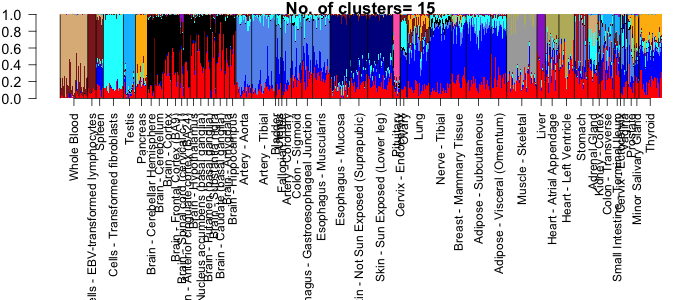
\includegraphics[height=3in, width=6.5in]{../plots/whole_tissue_structure_15.png}
%        \caption{Structure plot of the admixture proportions (with 15 topics/clusters) for all the tissue samples in GTEX Version 4 data based on $5000$ genes with the highest mean expression. Some of the tissues form very distinct clusters, for instance Whole Blood, Pancreas, Skin, Arteries etc while there is a lot of similarity in cluster patterns between Muscle Skeletal and Heart Left Ventricle, or among the different sub-tissues of the Brain.}
%\end{figure*}

\begin{sidewaysfigure*}[ht]
	\raggedleft
	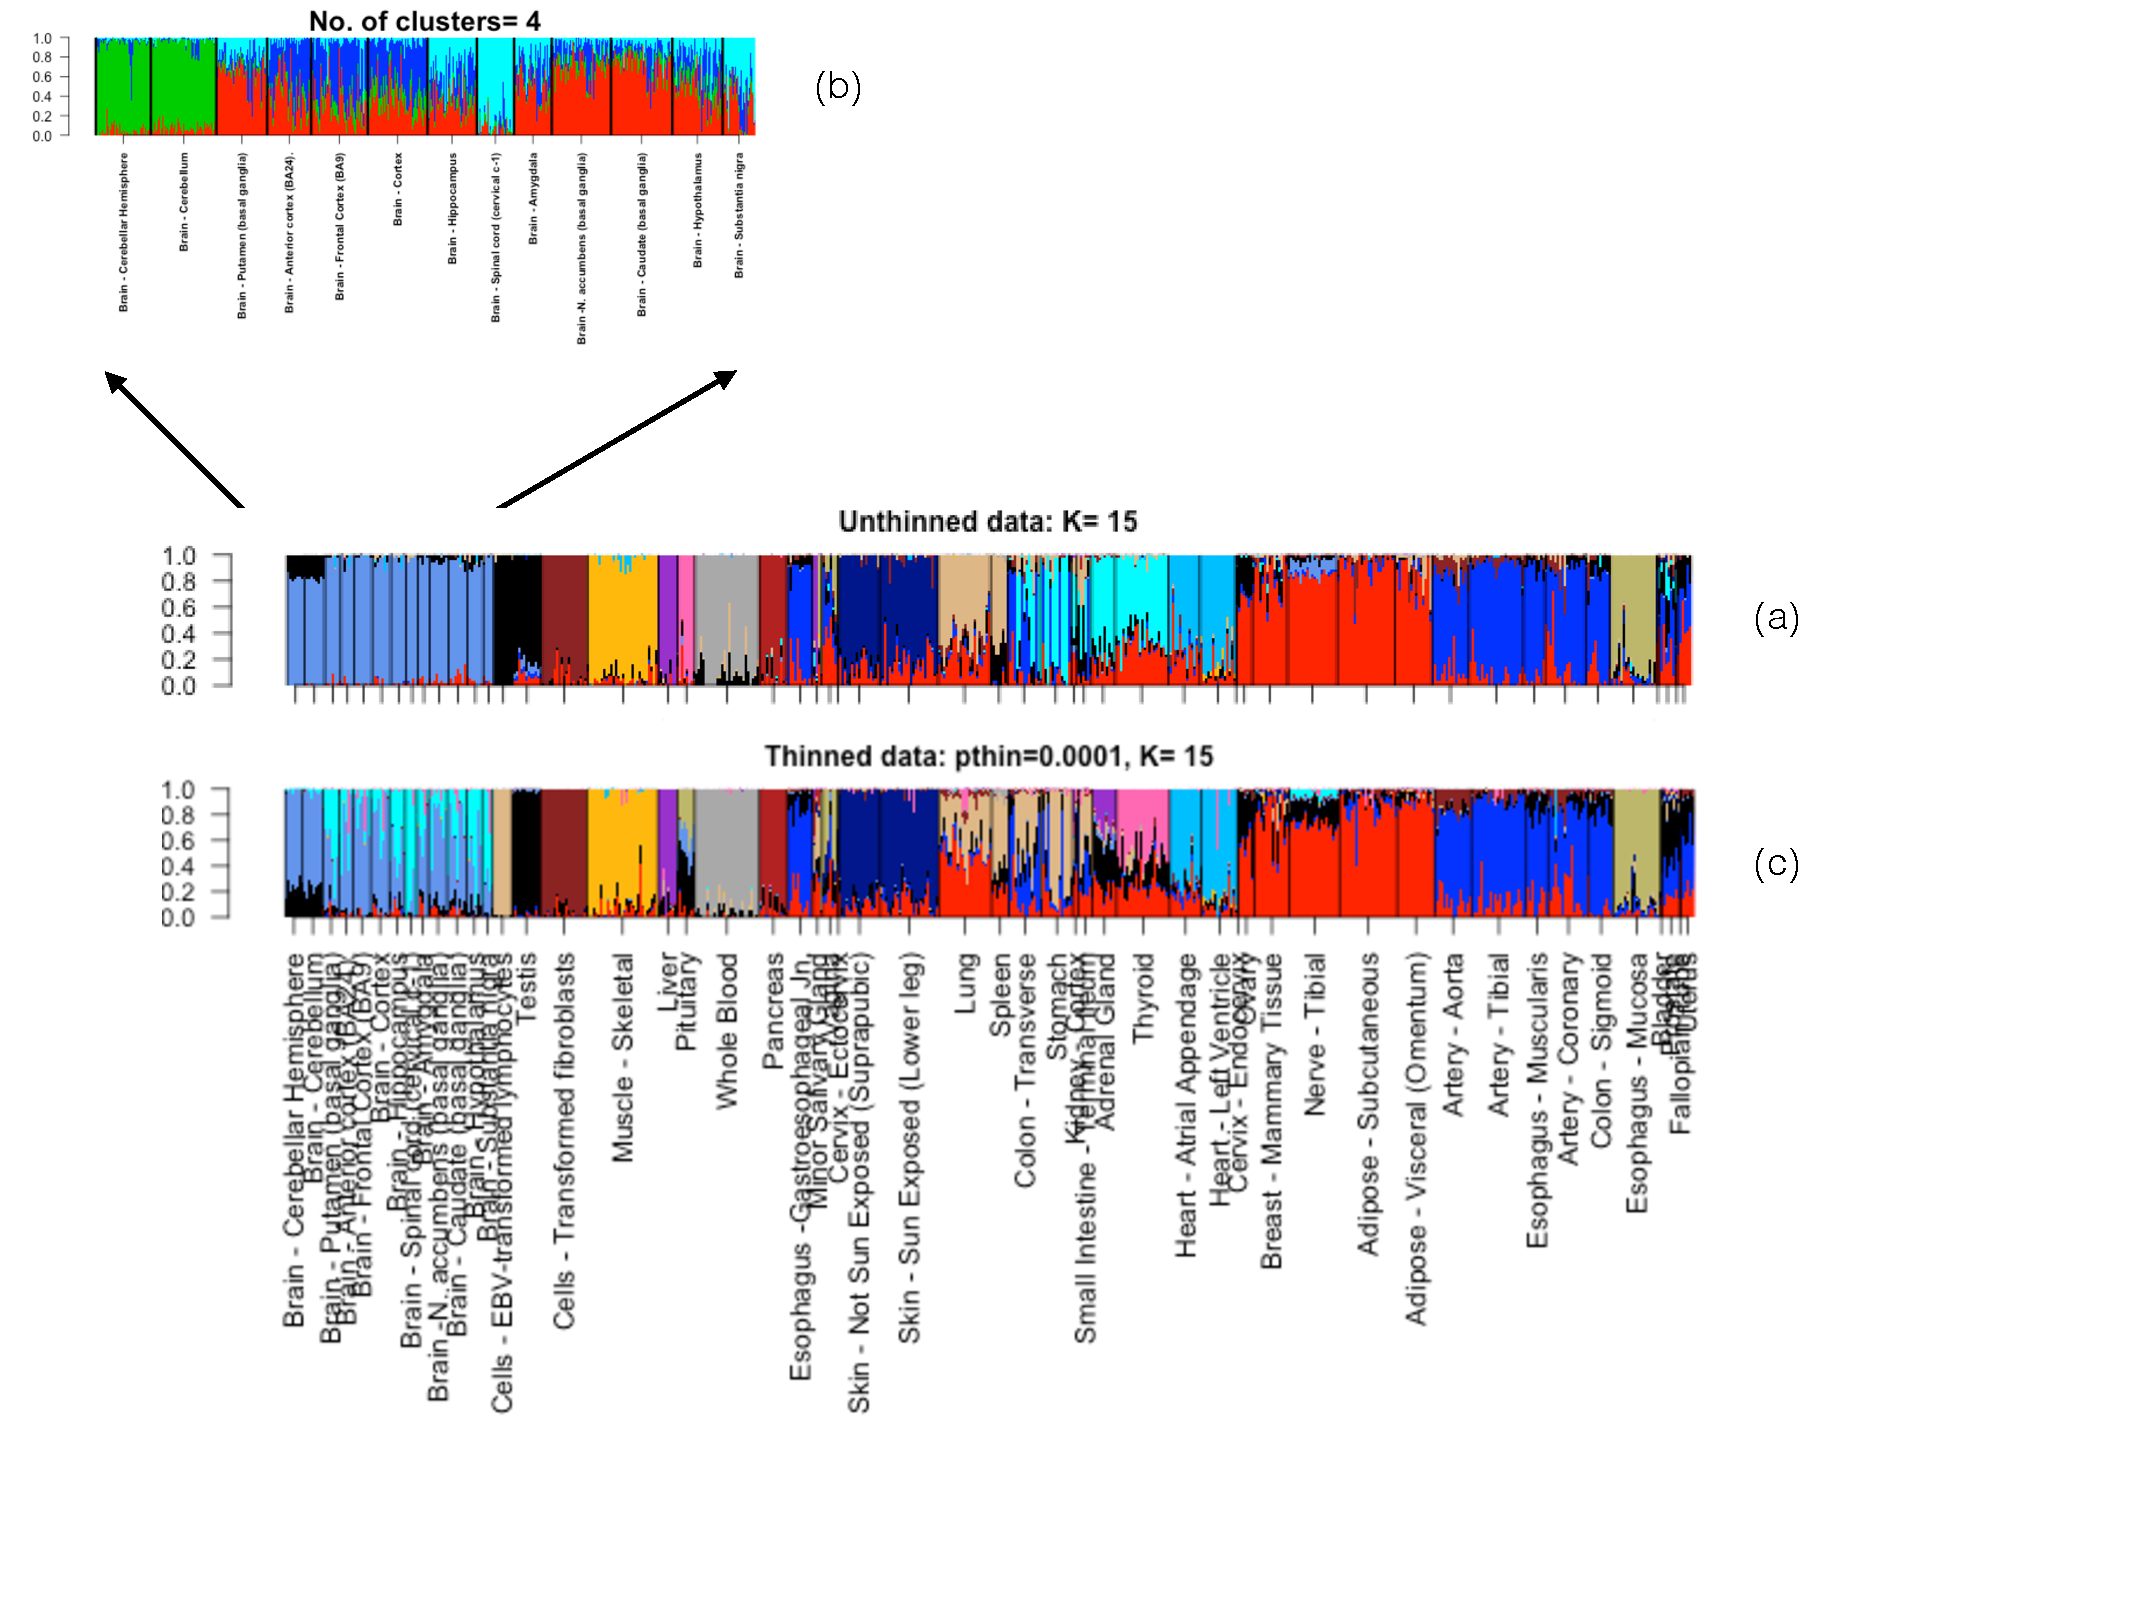
\includegraphics[height=5in, width=10.5in]{../plots/fig1_paper/fig1.pdf}
        \caption{ \textbf{(a)}: Structure plot of estimated cluster membership proportions for $K=15$ clusters fit to $8555$ tissue samples from $53$ tissues in GTEX data.  Each vertical bar shows the cluster membership proportions for a single sample, ordered with samples from the same tissue are adjacent to one another. \textbf{(b)}: Structure plot of estimated cluster membership proportions for $K=4$ clusters fit to just the brain tissue samples from GTEX. This analysis highlights structure among the brain samples that is absent from (a).  \textbf{(c)}: As in a), but with data thinned so that the coverage is closer to a typical single cell RNA-seq data ($p_{thin}=0.0001$).  The clustering patterns are largely similar to a), but slightly noisier.}
\label{fig:fig1}
\end{sidewaysfigure*}
%
%\begin{figure*}[ht]
%\centering
%  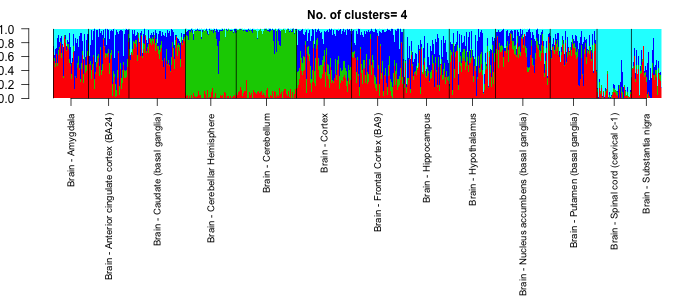
\includegraphics[height=3in, width=4.5in]{../plots/GTEX_V6_brain_thin_0.png}
%    \caption{Structure plot of the admixture proportions (with 4 clusters) for the brain tissue samples drawn from GTEX Version 4 data. Quite clearly, brain cerebellum and cerebellar hemisphere seem to be dominated by the blue cluster while the Spinal cord and Substantia nigra by the cyan cluster. Prior marker based approaches have verified that $> 80 \%$ of cells in brain cerebellum correspond to neurons \cite{Houzel2005}. So, the blue cluster seems to be driven by the neuron cell type. This fact is further attested by the gene annotations of the top genes driving the blue cluster (Supplementary Table 1).}
%\label{fig:fig2}
%\end{figure*}
%
% \begin{figure*}[ht]
%        \centering
%        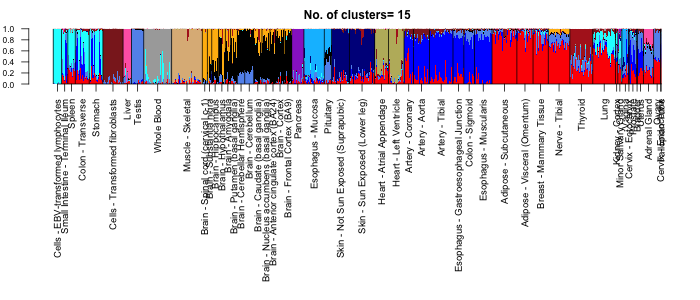
\includegraphics[height=2.7in]{../plots/GTEX_V6_thin_2.png}
%    \caption{Structure plot of all tissue samples in GTEx V6 data thinned data with $p_{thin}=0.0001$ for $K=15$. The thinning parameter has been chosen so that the GTEx RNA-seq data can be interpreted at the same scale as a scRNA-seq data.  The clustering patterns are more noisy compared to the non-thinned data in Fig \ref{fig:fig1}, but overall, the similarity patterns across the tissues are retained. For instance, the brain tissues and the arteries still seem to be clustering together.}
% \label{fig:fig4}
%    \end{figure*}


  \begin{figure*}[ht]
    \centering
    \begin{subfigure}[t]{0.5\textwidth}
        \centering
        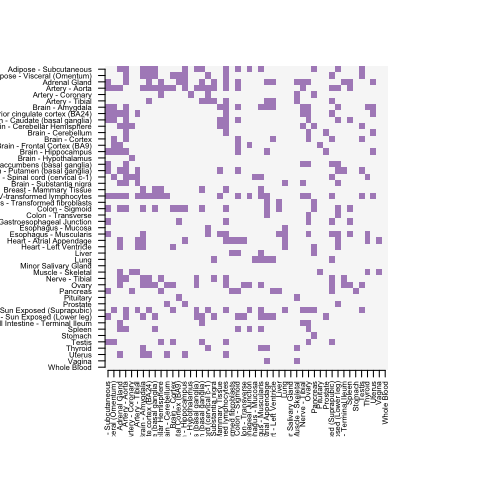
\includegraphics[height=2.5in]{../plots/hierarchy_F_thin_0_1.png}
        \caption{hierarchy thin 0.1}
    \end{subfigure}%
    ~ 
    \begin{subfigure}[t]{0.5\textwidth}
        \centering
        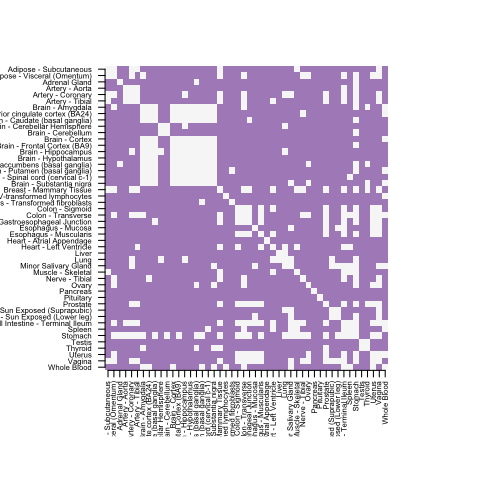
\includegraphics[height=2.5in]{../plots/admixture_F_thin_0_1.png}
        \caption{admixture thin 0.1}
    \end{subfigure} \\
\caption{A comparison of accuracy of hierarchical vs model-based clustering. For each pair of tissues, we selected randomly $50$ samples and then on the reads data for these $50$ samples, we applied the hierarchical clustering method with complete linkage and Euclidean distance and then cut the tree at $K=2$. We then observed if it separates out the samples coming from the two tissues, in case it does, we color the cell corresponding to that pair of tissues. We apply admixture model on the same data for $K=2$. Then we fixed one cluster, observed the proportions for that cluster, sorted the samples based on the proportions for that cluster and separated out the samples at the point of maximum jump/fall in the proportions for that cluster. If that separates out the two tissues, we color the cell, else keep it blank. From the graph it seems that the admixture model has been far more successful in separating out different tissues compared to the hierarchical method.}
\label{fig:fig2}
\end{figure*}


    
    
%     \begin{figure*}[ht]
%    \raggedright
%     \begin{subfigure}[t]{0.25\textwidth}
%        \raggedleft
%        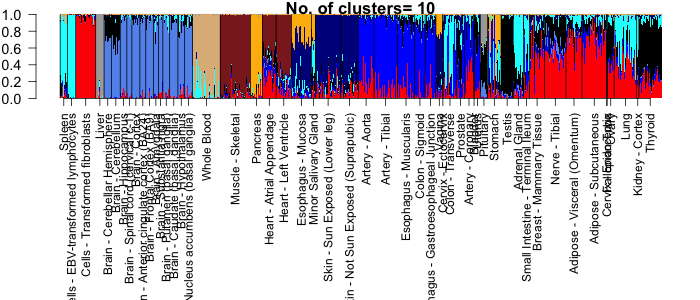
\includegraphics[height=2.5in]{../plots/multiple_thinned_1.png}
%        \caption{Run 1}
%    \end{subfigure}    \\
%    \begin{subfigure}[t]{0.25\textwidth}
%        \raggedleft
%        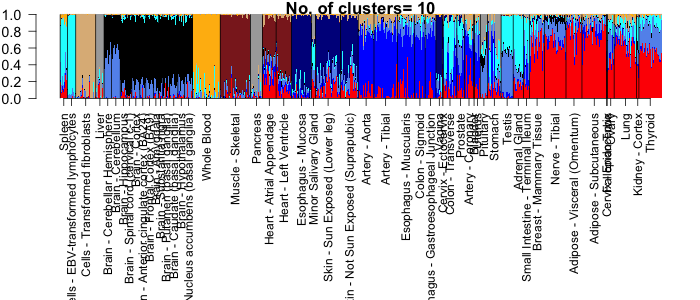
\includegraphics[height=2.5in]{../plots/multiple_thinned_2.png}
%        \caption{Run 2}
%    \end{subfigure}   \\
%    \begin{subfigure}[t]{0.25\textwidth}
%        \raggedleft
%        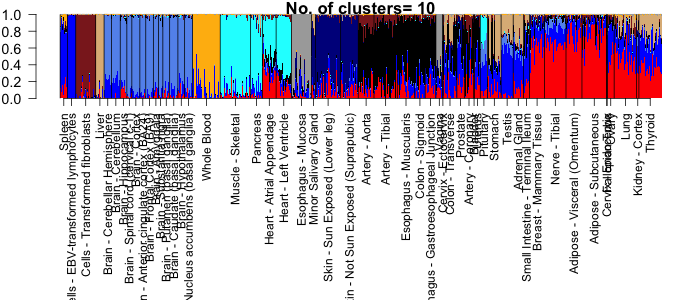
\includegraphics[height=2.5in]{../plots/multiple_thinned_4.png}
%        \caption{Run 3}
%    \end{subfigure} 
%    \caption{Structure plot of all tissue samples in 3 runs of the GTEx version 4 data for for K=10 for the thinning parameter $p_{thin}=0.01$. For the 3 runs, the datasets are randomly generated from the actual counts data using $p_{thin}=0.01$, so the datasets are different across the 3 runs. However, it seems the results are pretty robust.}
%    \end{figure*}
%
    
%    \begin{figure*}[ht]
%    \centering
%    \begin{subfigure}[t]{0.5\textwidth}
%        \centering
%        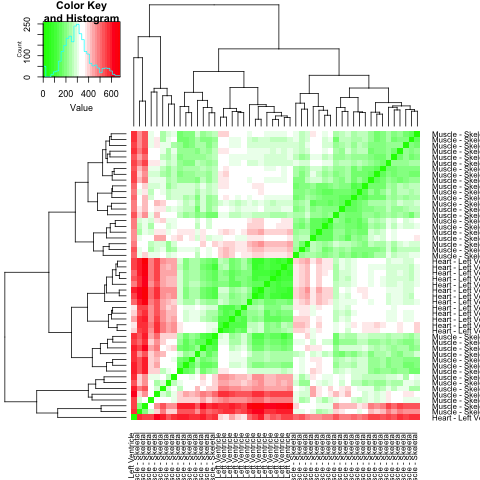
\includegraphics[height=2.5in]{../plots/heart_muscle_hierarchical_heatmap_complete.png}
%        \caption{counts- complete linkage}
%    \end{subfigure}%
%    ~ 
%    \begin{subfigure}[t]{0.5\textwidth}
%        \centering
%        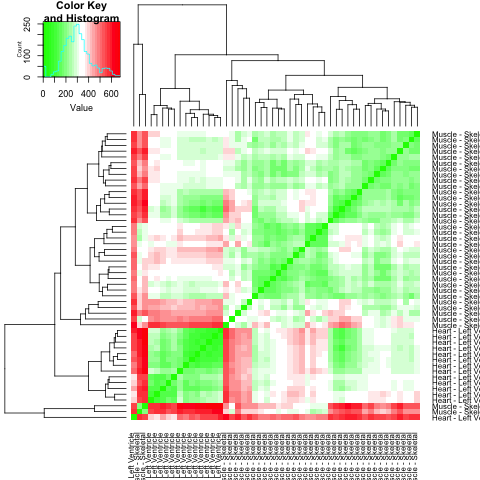
\includegraphics[height=2.5in]{../plots/heart_muscle_hierarchical_heatmap_average.png}
%        \caption{counts- average linkage}
%    \end{subfigure} \\
%    
%     \begin{subfigure}[t]{0.5\textwidth}
%        \centering
%        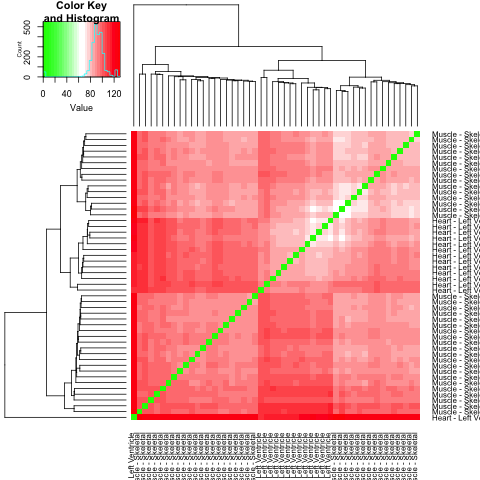
\includegraphics[height=2.5in]{../plots/heart_muscle_hierarchical_heatmap_cpm_complete.png}
%        \caption{cpm- complete linkage}
%    \end{subfigure}%
%    ~
%    \begin{subfigure}[t]{0.5\textwidth}
%        \centering
%        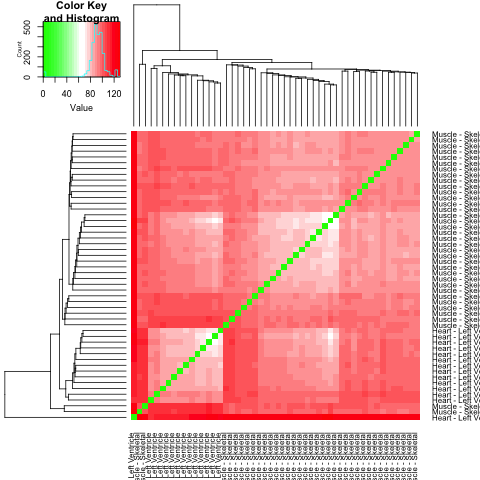
\includegraphics[height=2.5in]{../plots/heart_muscle_hierarchical_heatmap_cpm_average.png}
%        \caption{cpm- average linkage}
%    \end{subfigure}\\
%    
%     \begin{subfigure}[t]{0.5\textwidth}
%        \centering
%        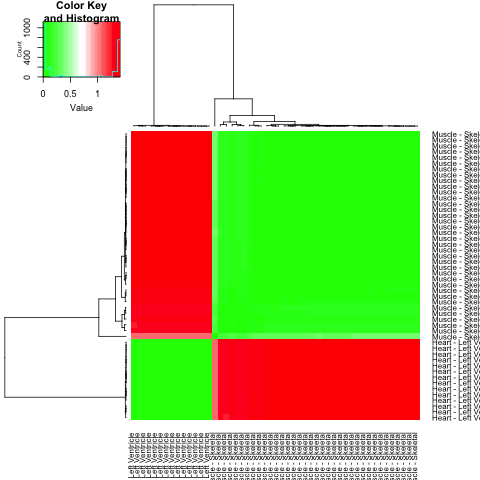
\includegraphics[height=2.5in]{../plots/heart_muscle_admix_heatmap_complete.png}
%        \caption{admix prop- complete linkage}
%    \end{subfigure}%
%    ~
%    \begin{subfigure}[t]{0.5\textwidth}
%        \centering
%        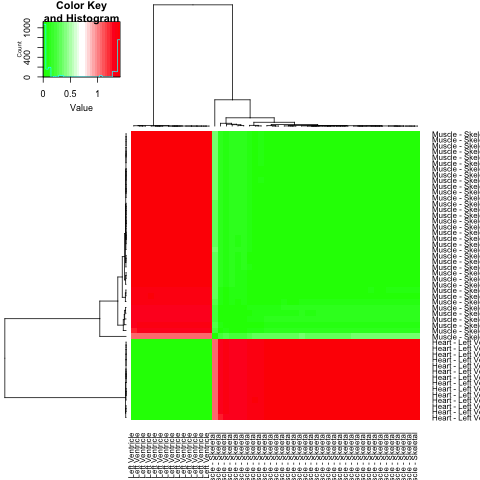
\includegraphics[height=2.5in]{../plots/heart_muscle_admix_heatmap_average.png}
%        \caption{admix prop- average linkage}
%    \end{subfigure}\\
%
%    \caption{Comparison of heatmap of the counts data (\textit{top panel}), the cpm normalized data (\textit{middle panel}) and the admixture proportions data (\textit{bottom panel}) on  a randomly drawn 50 samples from the pool of Muscle-Skeletal and Heart-Left Ventricle samples in GTEx Version 4 RNA-seq thinned counts data with the thinning parameter $p_{thin}=0.001$. The distance method used euclidean and the linkage used was average linkage. Color scale provided in the figure. It seems that for admixture model heatmap, all the Muscle-skeletal and Heart Left-Ventricle samples cluster separately, while for the hierarchical model heatmap, they are mixed with each other. This suggests Admixture is better equipped at picking tissue separation than hierarchical clustering.}
%\end{figure*}
%


%  \begin{figure*}[ht]
%    \centering
%    \begin{subfigure}[t]{0.5\textwidth}
%        \centering
%        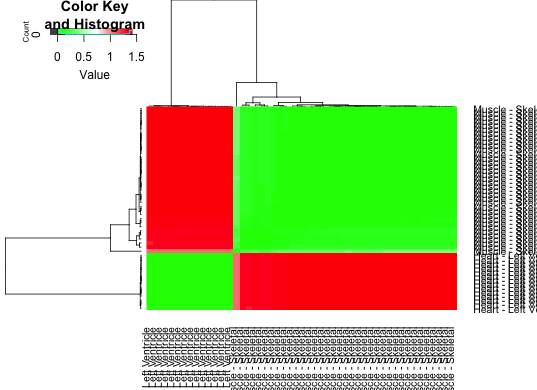
\includegraphics[height=2.5in]{../plots/hierarchical_admix_2.png}
%        \caption{k=2}
%    \end{subfigure}%
%    ~ 
%    \begin{subfigure}[t]{0.5\textwidth}
%        \centering
%        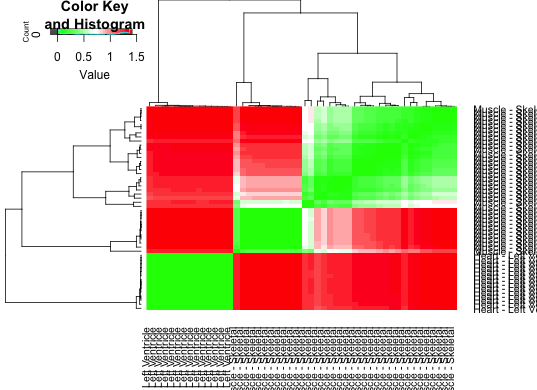
\includegraphics[height=2.5in]{../plots/hierarchical_admix_3.png}
%        \caption{k=3}
%    \end{subfigure} \\
%    
%     \begin{subfigure}[t]{0.5\textwidth}
%        \centering
%        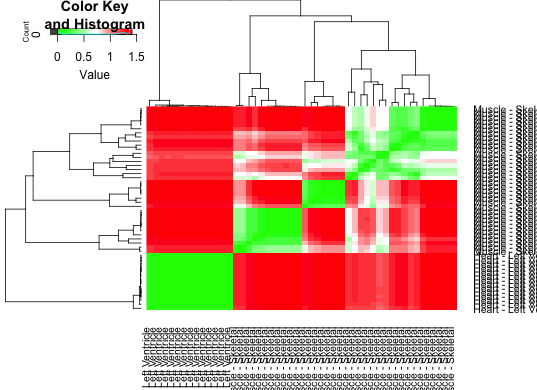
\includegraphics[height=2.5in]{../plots/hierarchical_admix_4.png}
%        \caption{k=4}
%    \end{subfigure}%
%    ~
%    \begin{subfigure}[t]{0.5\textwidth}
%        \centering
%        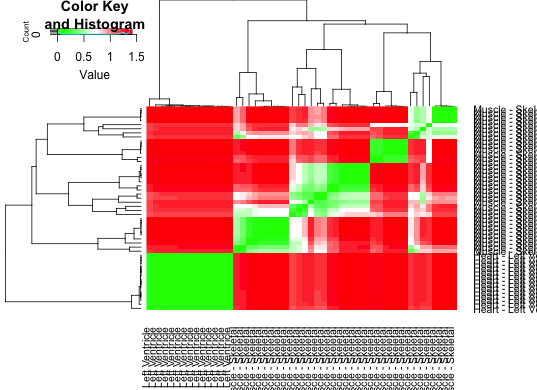
\includegraphics[height=2.5in]{../plots/hierarchical_admix_5.png}
%        \caption{k=5}
%    \end{subfigure}\\
%
% \caption{The heatmap of the admixture topic proportion matrix (low dimensional compared to the original counts data) under four different choices of clusters or topics namely $2,3,4$ and $5$. Here we assume complete linkage and the distance is taken to be Euclidean distance.}
%\end{figure*}

% \begin{figure*}[ht]
%    \centering
%    \begin{subfigure}[t]{0.5\textwidth}
%        \centering
%        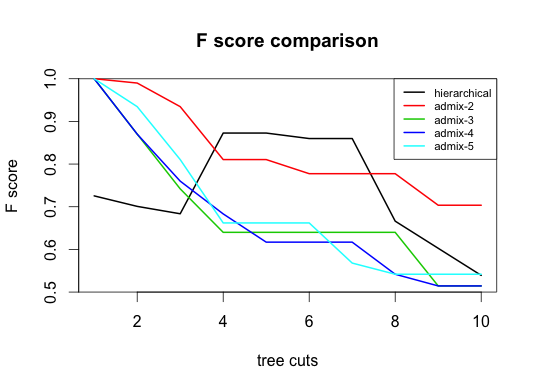
\includegraphics[height=2.5in]{../plots/Fscore_compare_average.png}
%        \caption{average linkage}
%    \end{subfigure}%
%    ~ 
%    \begin{subfigure}[t]{0.5\textwidth}
%        \centering
%        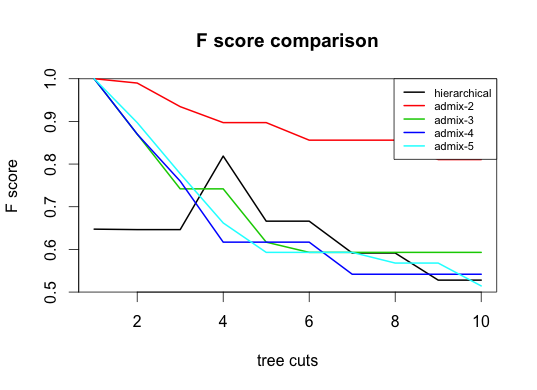
\includegraphics[height=2.5in]{../plots/Fscore_compare_complete.png}
%        \caption{complete linkage}
%    \end{subfigure} 
% \caption{The comparison of the F score of quality assessment between the hierarchical clustering on the actual counts data and the admixture model topic proportion matrix for number of topics $2$, $3$, $4$ and $5$. Higher values of $F$ imply better correspondence of the cluster labels with the pre-assigned class labels - in this case there being 2 classes, namely Muscle Skeletal and Heart Left Ventricle. The F scores are compared for both average and complete linkages.}
%\end{figure*}




%%\begin{figure*}[ht]
%    \centering
%    \begin{subfigure}[t]{0.5\textwidth}
%        \centering
%        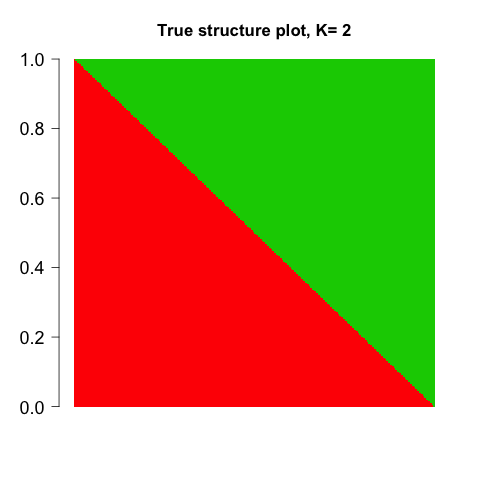
\includegraphics[height=3in]{../plots/true_structure_setup_1.png}
%        \caption{Set up 1 (true structure)}
%    \end{subfigure}%
%    ~ 
%    \begin{subfigure}[t]{0.5\textwidth}
%        \centering
%        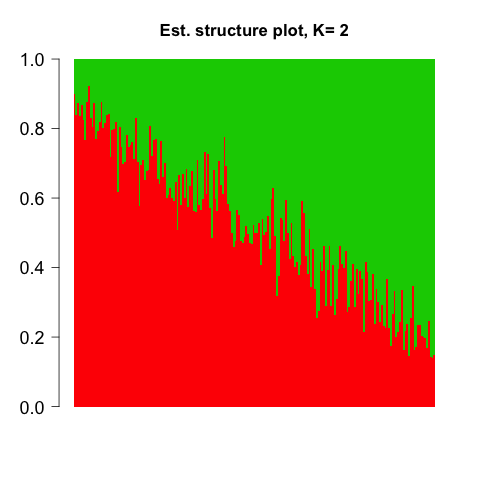
\includegraphics[height=3in]{../plots/est_structure_setup_1.png}
%        \caption{Set up 1 (est. structure)}
%    \end{subfigure}   \\
%    
%    \begin{subfigure}[t]{0.5\textwidth}
%        \centering
%        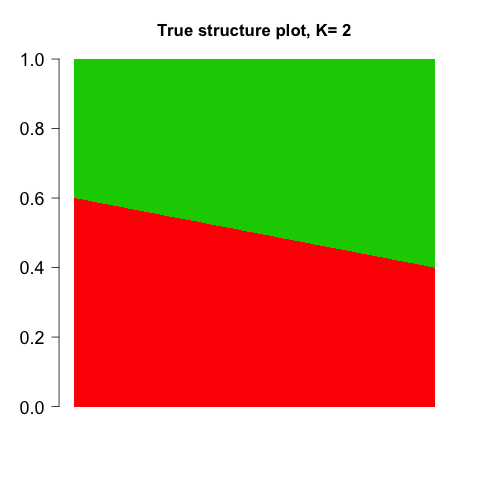
\includegraphics[height=3in]{../plots/true_structure_setup_2.png}
%        \caption{Set up 2 (true structure)}
%    \end{subfigure}%
%    ~ 
%    \begin{subfigure}[t]{0.5\textwidth}
%        \centering
%        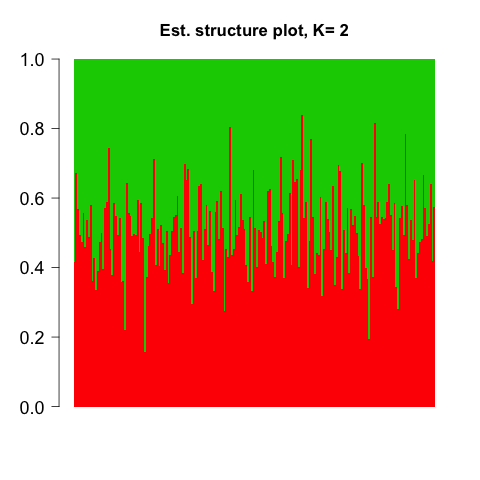
\includegraphics[height=3in]{../plots/est_structure_setup_2.png}
%        \caption{Set up 2 (est. structure)}
%    \end{subfigure} 
%    \caption{A case study to check for the performance of the admixture model under two set ups, one where the true admixture proportions vary a lot from 0 to 1 across samples for the two clusters and the other where the true admixture proportions vary mildly around $0.5$ (from $0.4$ to $0.6$) for the two clusters. It is found that the admixture model is able to distinguish the clusters better in the first set up compared to the second. Even from gene annotations point of view, it is found that the admixture model is able to extract the truly significantly enriched genes for the clusters in the first set up but fails to do so in the second set up.}
% \end{figure*}
% %
 
% \begin{figure*}[ht]
%    \centering
%    \begin{subfigure}[t]{0.5\textwidth}
%        \centering
%        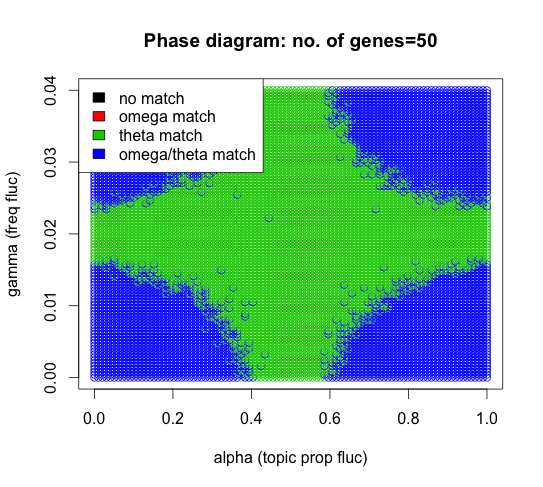
\includegraphics[height=3in]{../plots/phase_plot_50.png}
%        \caption{G=50}
%    \end{subfigure}%
%  ~ 
%    \begin{subfigure}[t]{0.5\textwidth}
%        \centering
%        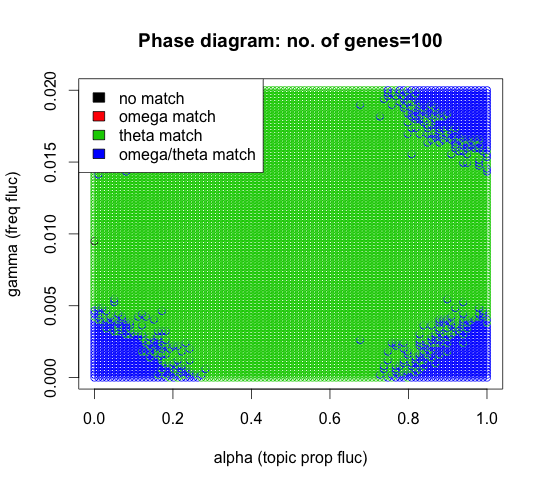
\includegraphics[height=3in]{../plots/phase_plot_100.png}
%        \caption{G=100}
%    \end{subfigure}   
%      ~ 
%    \begin{subfigure}[t]{0.5\textwidth}
%        \centering
%        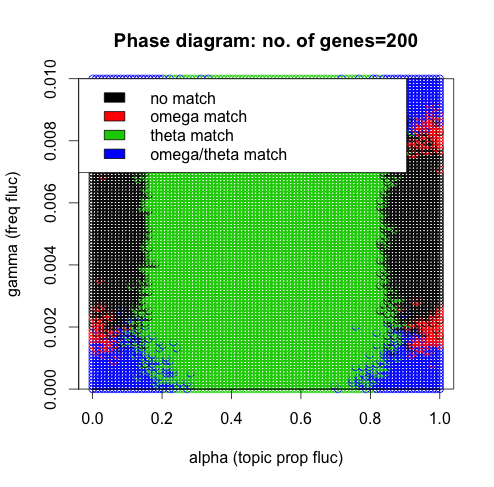
\includegraphics[height=3in]{../plots/phase_plot_200.png}
%        \caption{G=200}
%    \end{subfigure}   
%    \caption{Phase diagram analysis for number of samples $N=200$ and three choices of $G$, $50$, $100$ and $200$. Note that as $G$ increases, the gene expression signal and the distance between the relative gene expression between the two clusters decreases. As a result, the performance of the admixture model deteriorates. Also, for a broad part of the phase space, though the admixture model does not manage to determine the admixture proportions well enough (\textit{omega match} does not hold) but it is able to extract the actually important genes driving the clusters (\textit{theta match} holds).}
%    \end{figure*}
%    
 
% \begin{figure*}[ht]
%    \centering
%    \begin{subfigure}[t]{0.5\textwidth}
%        \centering
%        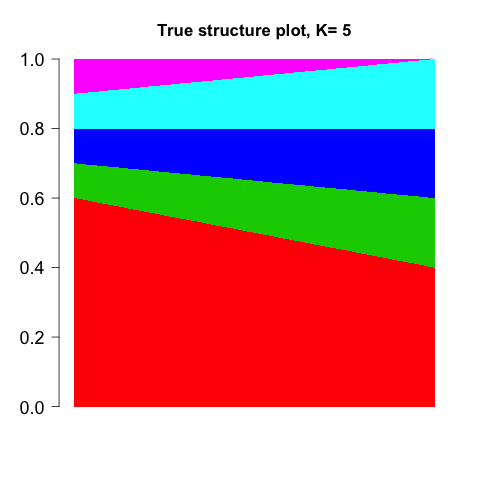
\includegraphics[height=3in]{../plots/true_structure_setup_3.png}
%        \caption{Set up 3 (true structure)}
%    \end{subfigure}%
%    ~ 
%    \begin{subfigure}[t]{0.5\textwidth}
%        \centering
%        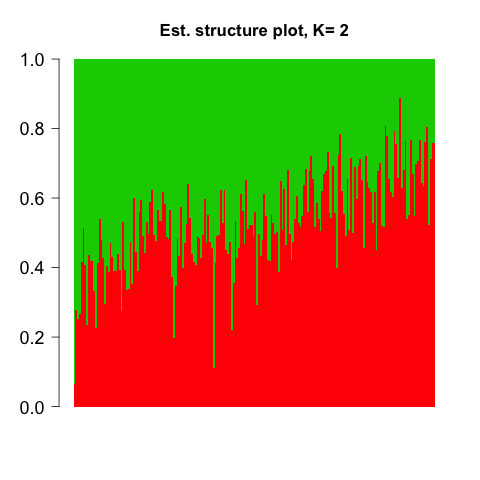
\includegraphics[height=3in]{../plots/est_structure_setup_3.png}
%        \caption{Set up 3 (est. structure)}
%    \end{subfigure}
%    \caption{The true structure plot for a simulation set up with $N=1000$ samples nd $G=500$ genes with $K=5$ clusters where the admixture proportions are given in (a). Counts data were generated under this true simulation set up. Then admixture model was fitted for $K=2$ and the estimated Structure plot from the model fit is shown in (b).}
%\end{figure*}

%\clearpage
%
%\begin{figure*}[ht]
%    \centering
%    \begin{subfigure}[t]{0.5\textwidth}
%        \centering
%        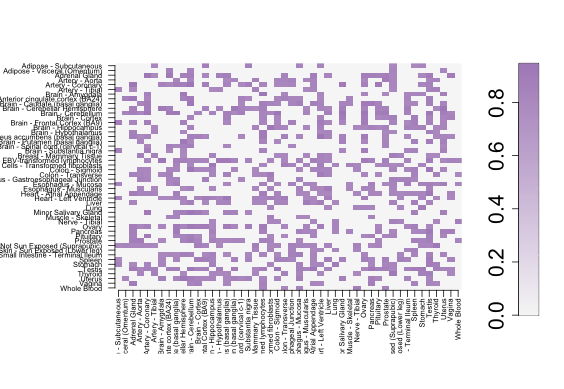
\includegraphics[height=2.5in,width=2.5in]{../plots/hierarchy_F_thin_clus_5_0_1.png}
%        \caption{hierarchy thin 0.1}
%    \end{subfigure}%
%    ~ 
%    \begin{subfigure}[t]{0.5\textwidth}
%        \centering
%        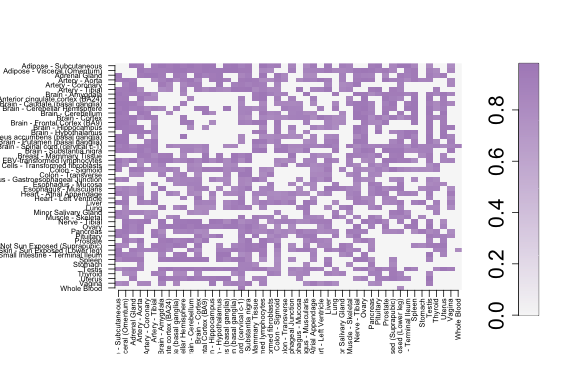
\includegraphics[height=2.5in,width=2.5in]{../plots/admixture_F_thin_clus_5_0_1.png}
%        \caption{admixture thin 0.1}
%    \end{subfigure} \\
%    
%     \begin{subfigure}[t]{0.5\textwidth}
%        \centering
%        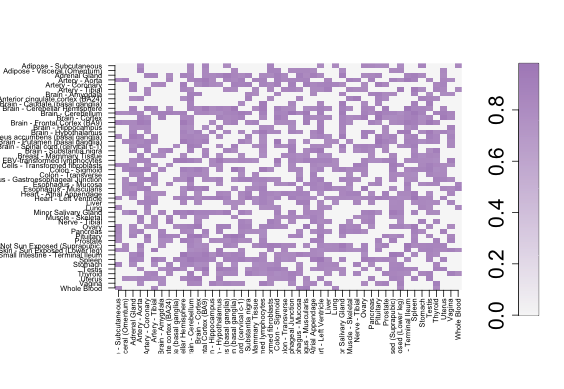
\includegraphics[height=2.5in,width=2.5in]{../plots/hierarchy_F_thin_clus_5_0_01.png}
%        \caption{hierarchy thin 0.01}
%    \end{subfigure}%
%    ~
%    \begin{subfigure}[t]{0.5\textwidth}
%        \centering
%        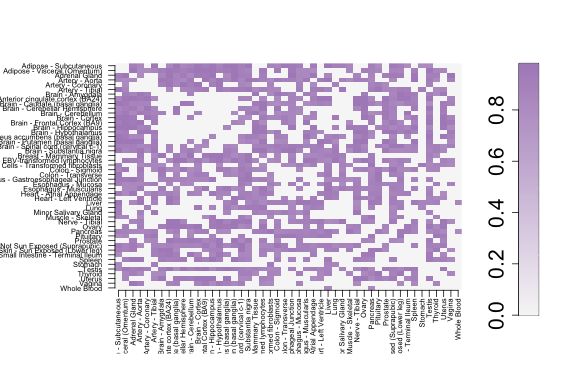
\includegraphics[height=2.5in,width=2.5in]{../plots/admixture_F_thin_clus_5_0_01.png}
%        \caption{admixture thin 0.01}
%    \end{subfigure}\\
%    
%     \begin{subfigure}[t]{0.5\textwidth}
%        \centering
%        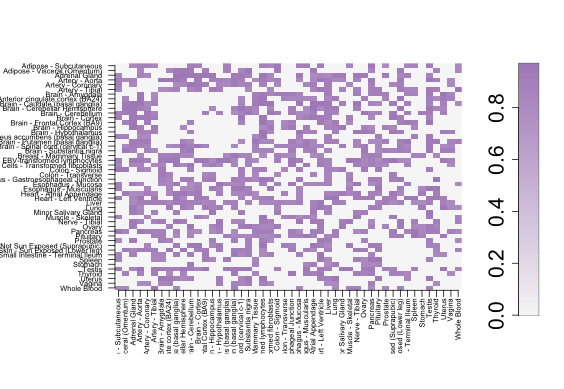
\includegraphics[height=2.5in,width=2.5in]{../plots/hierarchy_F_thin_clus_5_0_001.png}
%        \caption{hierarchy 0.001}
%    \end{subfigure}%
%    ~
%    \begin{subfigure}[t]{0.5\textwidth}
%        \centering
%        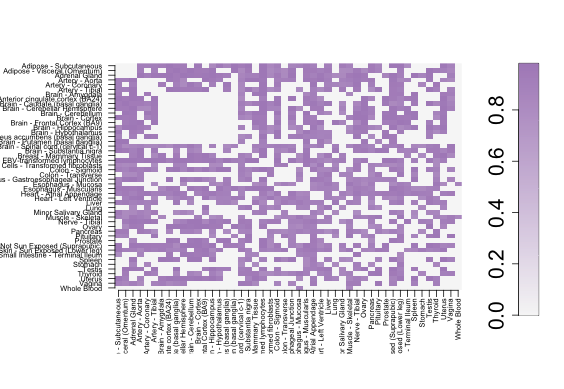
\includegraphics[height=2.5in,width=2.5in]{../plots/admixture_F_thin_clus_5_0_001.png}
%        \caption{admixture thin 0.001}
%    \end{subfigure}\\
% \caption{F score comparison of hierarchical clustering cut at 2 clusters on the actual counts data and on admixture proportions matrix  with 5 topics, where the F score is thresholded at $0.8$. In terms of F score, the performance of the admixture model in separating out the two clusters is much better than the hierarchical model. Also it seems that as we increase thinning, the performance does indeed deteriorate, as is intuitive. However, the relative efficiency of admixture over hierarchical clustering is maintained at all levels of thinning.}
%\end{figure*}
%
%

% \begin{figure*}[ht]
%    \raggedright
%     \begin{subfigure}[t]{0.3\textwidth}
%        \raggedleft
%        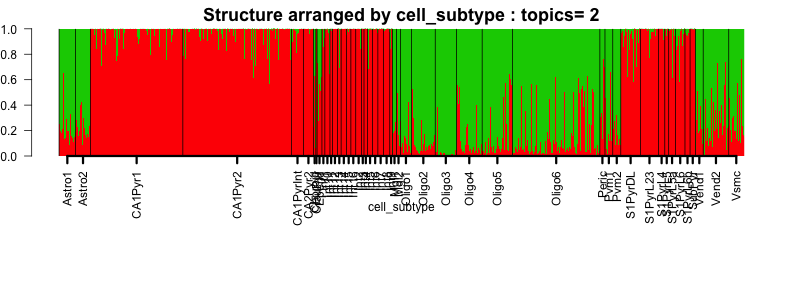
\includegraphics[height=2.5in]{../plots/Zeisel/clus_2/struct_clus_2_cell_subtype.png}
%        \raggedright 
%        \vspace{-0.5in} \qquad  \qquad  \caption{$k=2$}
%    \end{subfigure}    \\
%    \begin{subfigure}[t]{0.5\textwidth}
%        \raggedleft
%        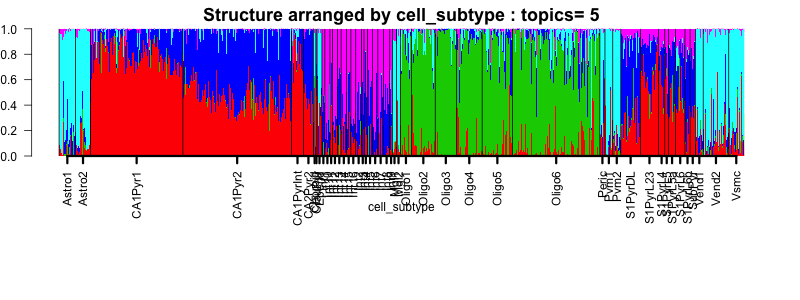
\includegraphics[height=2.5in]{../plots/Zeisel/clus_5/struct_clus_5_cell_subtype.png}
%        \raggedright
%        \vspace{-0.5in}  \qquad  \qquad \caption{$k=5$}
%    \end{subfigure}    \\
%    \begin{subfigure}[t]{0.5\textwidth}
%        \raggedleft
%        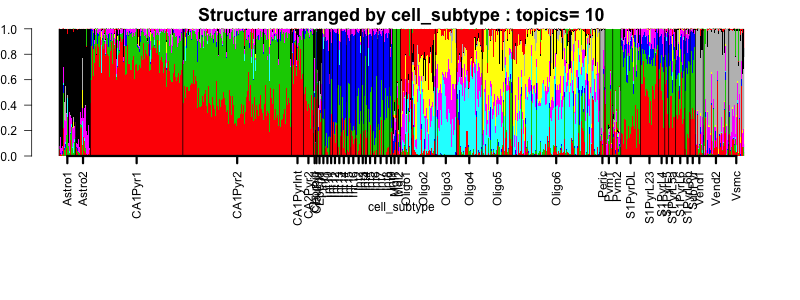
\includegraphics[height=2.5in]{../plots/Zeisel/clus_10/struct_clus_10_cell_subtype.png}
%        \raggedright
%        \vspace{-0.5in}  \qquad \qquad \caption{   $k=10$}
%    \end{subfigure}    
%    \caption{Structure plot of all  samples in Zeisel et al data \cite{Zeisel2015} arranged by the cell subtype labels that were determined by the authors using their BackSpin algorithm and subsequent marker gene annotations. Here we present the Structure plots for number of topics $k=2,5,10$. }
%    \end{figure*}


% \begin{figure*}[ht]
%    \raggedright
%     \begin{subfigure}[t]{1\textwidth}
%        \centering
%        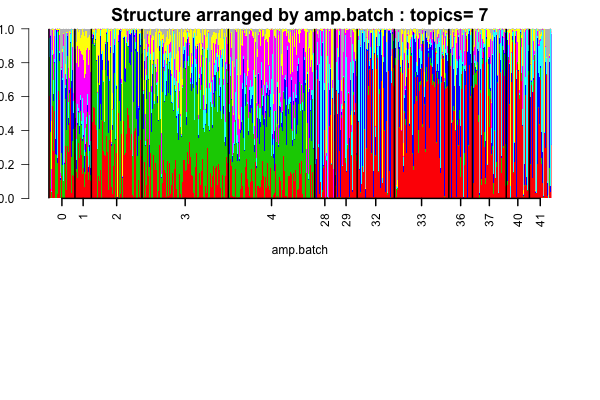
\includegraphics[height=2.5in, width=4.5in]{../plots/Jaitin_struct_clus_7_amp_batch.png}
%        \vspace{-1in} \qquad  \qquad  
%    \end{subfigure}    \\
%    \begin{subfigure}[t]{1\textwidth}
%       \centering
%        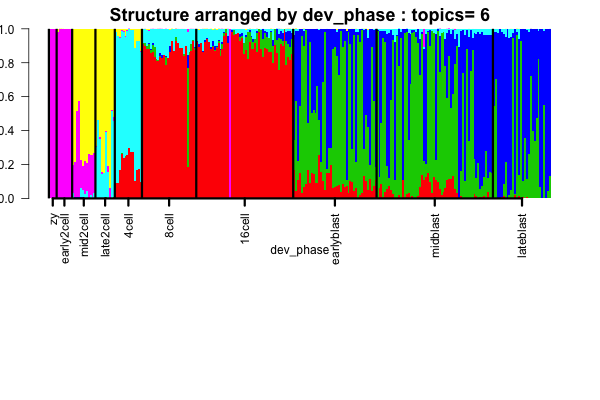
\includegraphics[height=2.5in, width=4.5in]{../plots/deng_structure_6.png}
%        \vspace{-0.5in}  \qquad \qquad 
%      \end{subfigure}
%    \caption{ (\textit{top panel})  Structure plot of the1041 single cells for K=7 of the Jaitin \textit{et al} data \cite{Jaitin2014} arranged by the amplification batch. It is observed that the clustering patterns within each batch are similar and so, either the amplification batch is driving the clustering or it is confounded with the actual biological effects, making it difficult to interpret these clusters. (\textit{bottom panel}) Structure plot of all samples for $K=6$ of Deng et al data \cite{Deng2014}, arranged by the preimplantation development phases of the cells and within each phase, arranged in the same order as in the data. Some developmental phases are represented by a single cluster, for example- \textit{zygote/early2cell} while some developmental phases can be written as a mix of two clusters or more clusters.}. 
% \label{fig:fig3}
% \end{figure*}
% 

\begin{figure*}[ht]
\centering
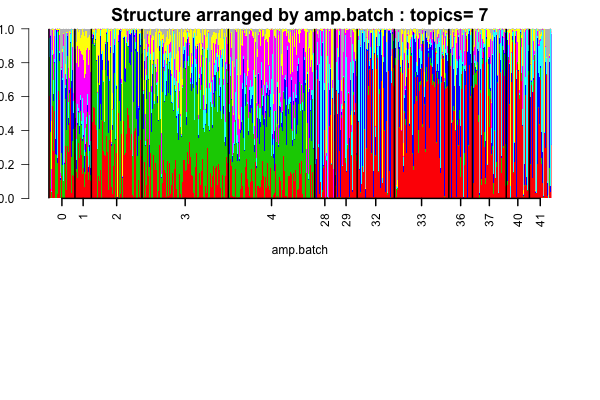
\includegraphics[height=2.5in, width=4.5in]{../plots/Jaitin_struct_clus_7_amp_batch.png}
\caption{ Structure plot of the1041 single cells for K=7 of the Jaitin \textit{et al} data \cite{Jaitin2014} arranged by the amplification batch. It is observed that the clustering patterns within each batch are similar and so, either the amplification batch is driving the clustering or it is confounded with the actual biological effects, making it difficult to interpret these clusters.}
\label{fig:fig3}
\end{figure*}



\begin{figure*}[ht]
\centering
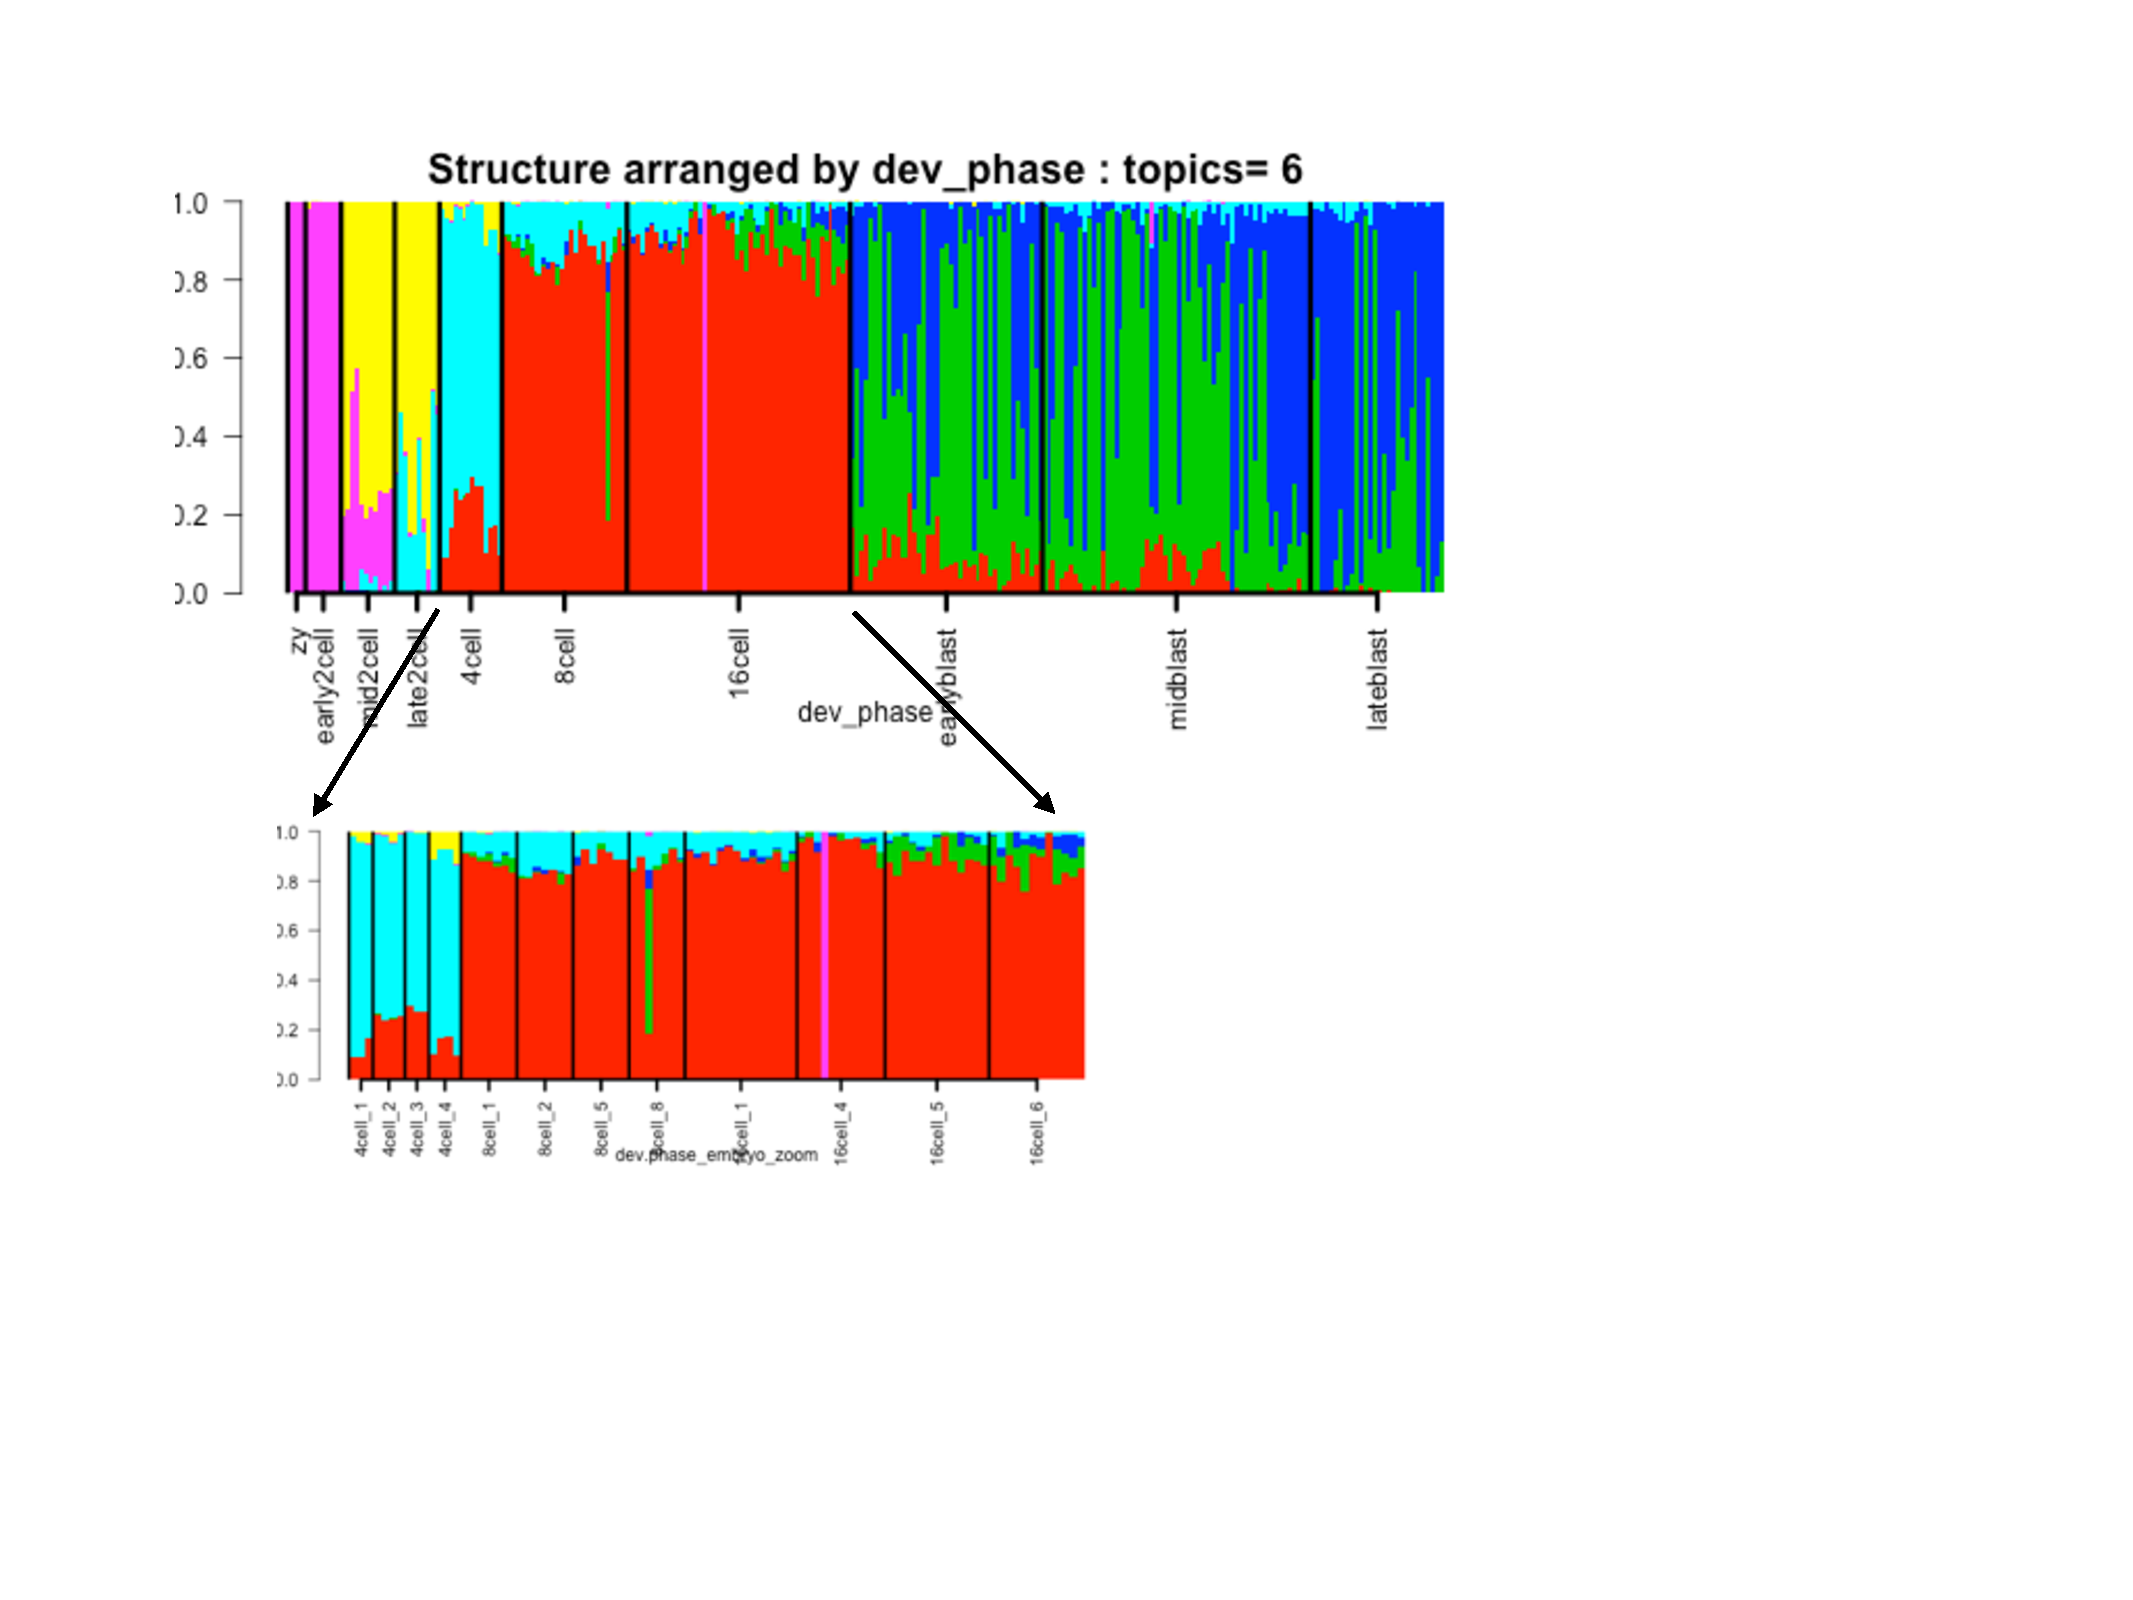
\includegraphics[height=4in, width=5.5in]{../plots/deng_structure_6.pdf}
\caption{ Structure plot of all samples for $K=6$ of Deng et al data \cite{Deng2014}, arranged by the preimplantation development phases of the cells and within each phase, arranged in the same order as in the data. Some developmental phases are represented by a single cluster, for example- \textit{zygote/early2cell} while some developmental phases can be written as a mix of two clusters or more clusters.}
\label{fig:fig4}
\end{figure*}


 \clearpage
 
 \subsection{Supplemental figures}
 
  \begin{figure*}[ht]
    \centering    
     \begin{subfigure}[t]{0.5\textwidth}
        \centering
        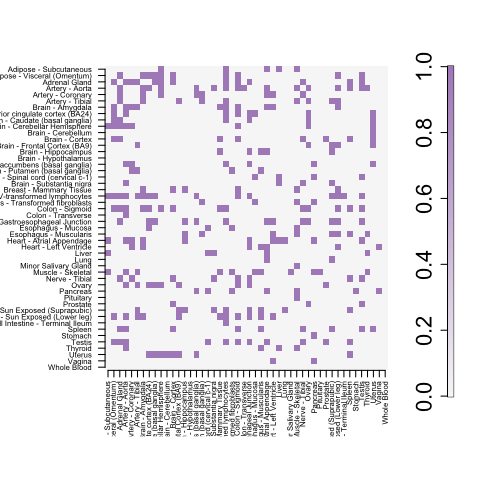
\includegraphics[height=2.5in]{../plots/hierarchy_F_thin_0_01.png}
        \caption{hierarchy thin 0.01}
    \end{subfigure}%
    ~
    \begin{subfigure}[t]{0.5\textwidth}
        \centering
        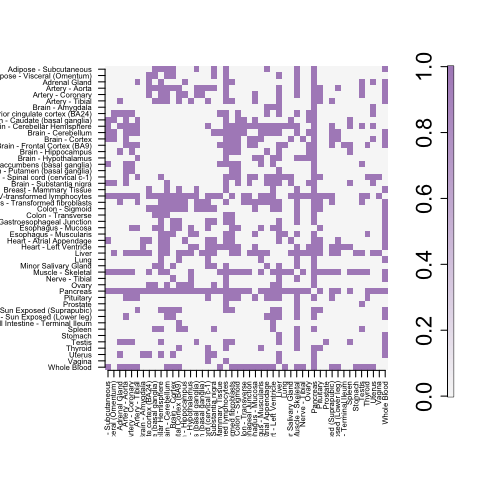
\includegraphics[height=2.5in]{../plots/admixture_F_thin_0_01.png}
        \caption{admixture thin 0.01}
    \end{subfigure}\\
    
     \begin{subfigure}[t]{0.5\textwidth}
        \centering
        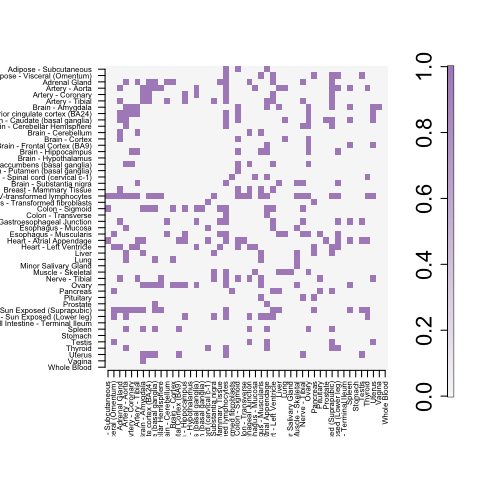
\includegraphics[height=2.5in]{../plots/hierarchy_F_thin_0_001.png}
        \caption{hierarchy 0.001}
    \end{subfigure}%
    ~
    \begin{subfigure}[t]{0.5\textwidth}
        \centering
        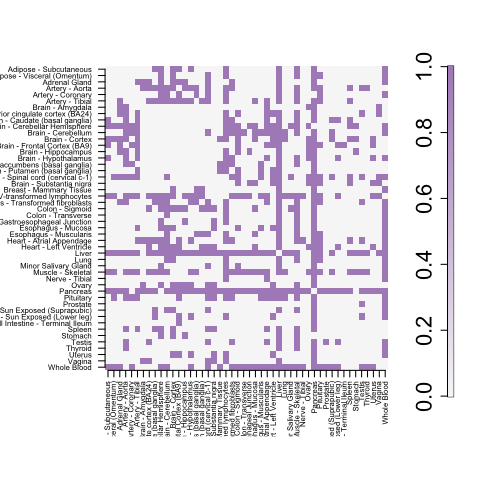
\includegraphics[height=2.5in]{../plots/admixture_F_thin_0_001.png}
        \caption{admixture thin 0.001}
    \end{subfigure}\\

    \caption{In this graph, we compare the hierarchical clustering method with the admixture method for thinned data with thinning parameters being $p_{thin}=0.001$ and $p_{thin}=0.0001$. The color coding scheme is similar to \textbf{Fig \ref{fig:fig2}}. Note that the performance of the admixture indeed deteriorates from \textbf{Fig \ref{fig:fig2}} in separating out the clusters as is expected. But it still outperforms the hierarchical clustering.}
 \label{fig:figS2}
\end{figure*}



%\clearpage
\begin{table}[htdp]
\begin{center}
\begin{tabular}{|c|p{0.5in}|p{1.4in}|p{3.6in}|} 
\hline
Cluster & Gene names & Proteins  & Summary \\
\hline

 \multirow{3}{4em}{\small{cluster red (Nerve, Adipose)} } &  \small{FABP4} & \footnotesize{ fatty acid binding protein 4, adipocyte} & \scriptsize{FABP4 encodes the fatty acid binding protein found in adipocytes, roles include fatty acid uptake, transport, and metabolism}\\ 
 					      & \small{APOD} & \footnotesize{apolipoprotein D} & \scriptsize{encodes a component of high density lipoprotein that has no marked similarity to other apolipoprotein sequences, closely associated with lipoprotein metabolism.}\\
					      & \small{PLIN1} & \footnotesize{perilipin} 1 & \scriptsize{coats lipid storage droplets in adipocytes, thereby protecting them until they can be broken down by hormone-sensitive lipase.} \\
 \hline
 \multirow{3}{4em}{\small{cluster blue (Arteries, Esophagus)} } & \small{MYH11} & \footnotesize{myosin, heavy chain 11, smooth muscle} & \scriptsize{functions as a major contractile protein, converting chemical energy into mechanical energy through the hydrolysis of ATP.} \\
 					    & \small{ACTA2} & \footnotesize{actin, alpha 2, smooth muscle, aorta} & \scriptsize{protein encoded by this gene belongs to the actin family of proteins, which are highly conserved proteins that play a role in cell motility, structure and integrity, defects in this gene cause aortic aneurysm familial thoracic type 6.}\\
					    &  \small{ACTG2} & \footnotesize{actin, gamma 2, smooth muscle, enteric} & \scriptsize{encodes actin gamma 2; a smooth muscle actin found in enteric tissues, involved in various types of cell motility and in the maintenance of the cytoskeleton. }\\
 \hline
 \multirow{3}{4em}{\small{cluster shallow blue (Brain)}} & \small{MBP} & \footnotesize{myelin basic protein} & \scriptsize{major constituent of the myelin sheath of oligodendrocytes and Schwann cells in the nervous system} \\
 					    & \small{GFAP} & \footnotesize{glial fibrillary acidic protein} & \scriptsize{encodes one of the major intermediate filament proteins of mature astrocytes, mutations casuses Alexander disease.} \\
					    & \small{SNAP25}  & \footnotesize{synaptosomal-associated protein, 25kDa} & \scriptsize{this gene product is a presynaptic plasma membrane protein involved in the regulation of neurotransmitter release.}\\
\hline
 \multirow{3}{4em}{\small{cluster black (Testis)}} & \small{PRM2} & \footnotesize{protamine 2} & \scriptsize{Protamines are the major DNA-binding proteins in the nucleus of sperm} \\
 					      & \small{PRM1} & \footnotesize{protamine 1} & \scriptsize{Protamines are the major DNA-binding proteins in the nucleus of sperm}  \\
					      & \small{PHF7} & \footnotesize{PHD finger protein 7} & \scriptsize{This gene is expressed in the testis in Sertoli cells but not germ cells, regulates spermatogenesis.} \\
\hline					      					      
 \multirow{3}{4em}{\small{cluster light blue (Thyroid, Stomach}} & \small{TG} & \footnotesize{thyroglobulin} & \scriptsize{thyroglobulin produced predominantly in thyroid gland, synthesizes thyroxine and triiodothyronine, associated with Graves disease and Hashimotot thyroiditis.} \\
 					     & \small{LIPF} & \footnotesize{lipase, gastric} & \scriptsize{encodes gastric lipase, an enzyme involved in the digestion of dietary triglycerides in the gastrointestinal tract, and responsible for 30 $\%$ of fat digestion processes occurring in human.} \\
					     & \small{PGC} & \footnotesize{progastricsin (pepsinogen C)} & \scriptsize{encodes an aspartic proteinase that belongs to the peptidase family A1. The encoded protein is a digestive enzyme that is produced in the stomach and constitutes a major component of the gastric mucosa,  associated with susceptibility to gastric cancers.}\\					     
 \hline
 \multirow{3}{4em}{\small{cluster deep blue (Skin)}} & \small{KRT10} & \footnotesize{keratin 10, type I} & \scriptsize{encodes a member of the type I (acidic) cytokeratin family, mutations associated with epidermolytic hyperkeratosis.}\\
 					    &  \small{KRT1} & \footnotesize{keratin 1, type II} & \scriptsize{specifically expressed in the spinous and granular layers of the epidermis with family member KRT10 and mutations in these genes have been associated with bullous congenital ichthyosiform erythroderma.} \\
					    & \small{KRT2} & \footnotesize{keratin 2, type II} & \scriptsize{expressed largely in the upper spinous layer of epidermal keratinocytes and mutations in this gene have been associated with bullous congenital ichthyosiform erythroderma.}\\
 \hline
 \multirow{3}{4em}{\small{cluster dark brown (Cells fibroblasts)}} & \small{FN1}  & \footnotesize{fibronectin 1} & \scriptsize{Fibronectin is involved in cell adhesion, embryogenesis, blood coagulation, host defense, and metastasis.} \\
 					      & \small{COL1A1} & \footnotesize{collagen, type I, alpha 1} & \scriptsize{Mutations in this gene associated with osteogenesis imperfecta types I-IV, Ehlers-Danlos syndrome type and Classical type, Caffey Disease}. \\
					      & \small{COL1A2} & \footnotesize{collagen, type I, alpha 2} & \scriptsize{Mutations in this gene associated with osteogenesis imperfecta types I-IV, Ehlers-Danlos syndrome type and Classical type, Caffey Disease}. \\
\hline
\end{tabular}
 \end{center}
 \label{tab:tab1}
\end{table}


%
%
%\begin{table}
%\newpage
%\begin{center}
%\begin{tabular}{|c|p{0.5in}|p{1.9in}|p{2.5in}|} 
%\hline
%Cluster & Gene names & Proteins  & Summary \\
%\hline
%
% \multirow{3}{4em}{cluster black (Testis)} & PRM2 & protamine 2 & \small{Protamines are the major DNA-binding proteins in the nucleus of sperm} \\
% 					      & PRM1 & protamine 1 & \small{Protamines are the major DNA-binding proteins in the nucleus of sperm}  \\
%					      & PHF7 & PHD finger protein 7 & \small{This gene is expressed in the testis in Sertoli cells but not germ cells, regulates spermatogenesis.} \\
%\hline					      					      
% \multirow{3}{4em}{cluster light blue (Thyroid, Stomach} & TG & thyroglobulin & \small{thyroglobulin produced predominantly in thyroid gland, synthesizes thyroxine and triiodothyronine, associated with Graves disease and Hashimotot thyroiditis.} \\
% 					     & LIPF & lipase, gastric & \small{encodes gastric lipase, an enzyme involved in the digestion of dietary triglycerides in the gastrointestinal tract, and responsible for 30 $\%$ of fat digestion processes occurring in human.} \\
%					     & PGC & progastricsin (pepsinogen C) & \small{encodes an aspartic proteinase that belongs to the peptidase family A1. The encoded protein is a digestive enzyme that is produced in the stomach and constitutes a major component of the gastric mucosa,  associated with susceptibility to gastric cancers.}\\					     
% \hline
% \multirow{3}{4em}{cluster deep blue (Skin)} & KRT10 & keratin 10, type I & \small{encodes a member of the type I (acidic) cytokeratin family, mutations associated with epidermolytic hyperkeratosis.}\\
% 					    &  KRT1 & keratin 1, type II & \small{specifically expressed in the spinous and granular layers of the epidermis with family member KRT10 and mutations in these genes have been associated with bullous congenital ichthyosiform erythroderma.} \\
%					    & KRT2 & keratin 2, type II & \small{expressed largely in the upper spinous layer of epidermal keratinocytes and mutations in this gene have been associated with bullous congenital ichthyosiform erythroderma.}\\
% \hline
% \multirow{3}{4em}{cluster dark brown (Cells fibroblasts)} & FN1  & fibronectin 1 & \small{Fibronectin is involved in cell adhesion, embryogenesis, blood coagulation, host defense, and metastasis.} \\
% 					      & COL1A1 & collagen, type I, alpha 1 & \small{Mutations in this gene associated with osteogenesis imperfecta types I-IV, Ehlers-Danlos syndrome type and Classical type, Caffey Disease}. \\
%					      & COL1A2 & collagen, type I, alpha 2 & \small{Mutations in this gene associated with osteogenesis imperfecta types I-IV, Ehlers-Danlos syndrome type and Classical type, Caffey Disease}. \\
%\hline	
% \end{tabular}
% \end{center}
%\end{table}
%




\newpage
\begin{table}
\begin{center}
\begin{tabular}{|c|p{0.5in}|p{1.4in}|p{3.6in}|}
\hline
Cluster & Gene names & Proteins  & Summary \\
\hline
\multirow{3}{4em}{\small{cluster shallow yellow (Lung)}} & \small{SFTPB} & \footnotesize{surfactant protein B} & \scriptsize {an amphipathic surfactant protein essential for lung function and homeostasis after birth, muttaions cause pulmonary alveolar proteinosis, fatal respiratory distress in the neonatal period.} \\
 					    & \small{SFTPA2} & \footnotesize{surfactant protein A2} & \scriptsize{Mutations in this gene and a highly similar gene located nearby, which affect the highly conserved carbohydrate recognition domain, are associated with idiopathic pulmonary fibrosis.} \\
					    & \small{SFTPA1} & \footnotesize{surfactant protein A1} &  \scriptsize{encodes a lung surfactant protein that is a member of C-type lectins called collectins, associated with idiopathic pulmonary fibrosis.} \\
\hline				   
 \multirow{3}{4em}{\small{cluster yellow (Muscle skeletal)}} & \small{MYH1} & \footnotesize{myosin, heavy chain 1, skeletal muscle, adult }& \scriptsize{a major contractile protein which converts chemical energy into mechanical energy through the hydrolysis of ATP.} \\
 					    & \small{NEB} & \footnotesize{nebulin} & \scriptsize{encodes nebulin, a giant protein component of the cytoskeletal matrix that coexists with the thick and thin filaments within the sarcomeres of skeletal muscle, associated with recessive nemaline myopathy.} \\
					    & \small{MYH2} & \footnotesize{myosin, heavy chain 2, skeletal muscle, adult} & \scriptsize{encodes a member of the class II or conventional myosin heavy chains, and functions in skeletal muscle contraction.} \\
\hline					    
 \multirow{3}{4em}{\small{cluster grey (Whole Blood)}} & \small{HBB} & \footnotesize{hemoglobin, beta} & \scriptsize{mutant beta globin causes sickle cell anemia, absence of beta chain/ reduction in beta globin leads to thalassemia.}\\
 					      & \small{HBA2} & \footnotesize{hemoglobin, alpha 2} & \scriptsize{deletion of alpha genes may lead to alpha thalassemia.}  \\
					      & \small{HBA1} & \footnotesize{hemoglobin, alpha 1} & \scriptsize{deletion of alpha genes may lead to alpha thalassemia.}  \\
\hline				      

 \multirow{3}{4em}{\small{cluster cyan (Heart)}} &  \small{NPPA} & \footnotesize{natriuretic peptide A} & \scriptsize{protein encoded by this gene belongs to the natriuretic peptide family, associated with atrial fibrillation familial type 6.} \\
 					      &  \small{MYH6} & \footnotesize{myosin, heavy chain 6, cardiac muscle, alpha} & \scriptsize{encodes the alpha heavy chain subunit of cardiac myosin, mutations in this gene cause familial hypertrophic cardiomyopathy and atrial septal defect 3.} \\
					      &  \small{ACTC1} & \footnotesize{actin, alpha, cardiac muscle 1} & \scriptsize{protein encoded by this gene belongs to the actin family, associated with idiopathic dilated cardiomyopathy (IDC) and familial hypertrophic cardiomyopathy (FHC).} \\
\hline			      
 \multirow{3}{4em}{\small{cluster shallow green (Esophagus mucosa)}} &  \small{KRT13} & \footnotesize{keratin 13, type I} & \scriptsize{protein encoded by this gene is a member of the keratin gene family, associated with the autosomal dominant disorder White Sponge Nevus.}\\
 					      &  \small{KRT4} & \footnotesize{keratin 4, type II} & \scriptsize{protein encoded by this gene is a member of the keratin gene family, associated with White Sponge Nevus, characterized by oral, esophageal, and anal leukoplakia.} \\
					      &  \small{CRNN} & \footnotesize{cornulin} & \scriptsize{may play a role in the mucosal/epithelial immune response and epidermal differentiation. } \\
\hline
 \multirow{3}{4em}{\small{cluster light brown (Pancreas)}} &  \small{PRSS1} & \footnotesize{protease, serine 1} & \scriptsize{secreted by pancreas, associated with pancreatitis}\\
 					      &  \small{CPA1} & \footnotesize{carboxypeptidase A1} & \scriptsize{secreted by pancreas, linked to pancreatitis and pancreatic cancer} \\
					      &  \small{PNLIP} & \footnotesize{pancreatic lipase} & \scriptsize{encodes a carboxyl esterase that hydrolyzes insoluble, emulsified triglycerides, and is essential for the efficient digestion of dietary fats. This gene is expressed specifically in the pancreas.}\\
\hline				      
 \multirow{3}{4em}{\small{cluster violet (Liver)}} &  \small{MUC7} & \footnotesize{mucin 7, secreted} & \scriptsize{encodes a small salivary mucin, thought to play a role in facilitating the clearance of bacteria in the oral cavity and to aid in mastication, speech, and swallowing, associated with susceptibility to asthma.} \\
 					      &  \small{ALB} & \footnotesize{albumin} & \scriptsize{functions primarily as a carrier protein for steroids, fatty acids, and thyroid hormones and plays a role in stabilizing extracellular fluid volume.} \\
					      &  \small{HP} & \footnotesize{haptoglobin} & \scriptsize{encodes a preproprotein, which subsequently  produces haptoglobin, linked to diabetic nephropathy, Crohn's disease, inflammatory disease behavior and reduced incidence of Plasmodium falciparum malaria.}\\
\hline					      
 \multirow{3}{4em}{\small{cluster salmon (Pituitary)}}&  \small{PRL} & \footnotesize{prolactin 2} & \scriptsize{encodes the anterior pituitary hormone prolactin. This secreted hormone is a growth regulator for many tissues, including cells of the immune system.} \\
 					      &  \small{GH1} & \footnotesize{growth hormone 1} & \scriptsize{expressed in the pituitary, play an important role in growth control, mutations in or deletions of the gene lead to growth hormone deficiency and short stature.}\\
					      &  \small{POMC} & \footnotesize{proopiomelanocortin} & \scriptsize{synthesized mainly in corticotroph cells of the anterior pituitary, mutations in this gene have been associated with early onset obesity, adrenal insufficiency, and red hair pigmentation.} \\
\hline
 \end{tabular}
 \end{center}
\end{table}

\clearpage

\subsection{Supplementary Table 1}

\begin{table}[htdp]
\begin{center}
\begin{tabular}{|c|p{0.5in}|p{1.4in}|p{3.6in}|} 
\hline
Cluster & Gene names & Proteins  & Summary \\
\hline
 \multirow{3}{4em}{\small{cluster 1,red}}  &  \small{ATP1A2} & \footnotesize{ ATPase, Na+/K+ transporting, alpha 2 polypeptide} & \scriptsize{responsible for establishing and maintaining the electrochemical gradients of Na and K ions across the plasma membrane, mutations in this gene result in familial basilar or hemiplegic migraines, and in a rare syndrome known as alternating hemiplegia of childhood.}   \\ 
 					      & \small{CLU} &  \footnotesize{clusterin} & \scriptsize{protein encoded by this gene is a secreted chaperone that can under some stress conditions also be found in the cell cytosol, also involved in cell death, tumor progression, and neurodegenerative disorders.} \\
					      & \small{DNAJB1} & \footnotesize{DnaJ (Hsp40) homolog, subfamily B, member 1} & \scriptsize{encodes a member of the DnaJ or Hsp40 (heat shock protein 40 kD) family of proteins, that stimulates the ATPase activity of Hsp70 heat-shock proteins  to promote protein folding and prevent misfolded protein aggregation.} \\
\hline
 \multirow{3}{4em}{\small{cluster 2, green}} & \small{SNAP25} & \footnotesize{synaptosomal-associated protein, 25kDa} & \scriptsize{Synaptic vesicle membrane docking and fusion is mediated by SNAREs located on the vesicle membrane (v-SNAREs) and the target membrane (t-SNAREs), involved in the regulation of neurotransmitter release.}\\
 					    & \small{ENO2} & \footnotesize{enolase 2 (gamma, neuronal)} & \scriptsize{ encodes one of the three enolase isoenzymes found in mammals, is found in mature neurons and cells of neuronal origin.} \\
					    &  \small{CHGB} &  \footnotesize{chromogranin B} & \scriptsize{ encodes a tyrosine-sulfated secretory protein abundant in peptidergic endocrine cells and neurons. This protein may serve as a precursor for regulatory peptides.} \\
 \hline
 
 \multirow{3}{4em}{\small{cluster 3,blue}}  &  \small{CALM3} & \footnotesize{calmodulin 3 (phosphorylase kinase, delta)} & \scriptsize{ is a calcium binding protein that plays a role in signaling pathways, cell cycle progression and proliferation.}   \\ 
 					      & \small{FBXL16} &  \footnotesize{F-box and leucine-rich repeat protein 16} & \scriptsize{ Members of the F-box protein family, such as FBXL16, are characterized by an approximately 40-amino acid F-box motif.} \\
					      & \small{UCHL1} & \footnotesize{ubiquitin carboxyl-terminal esterase L1} & \scriptsize{specifically expressed in the neurons and in cells of the diffuse neuroendocrine system. Mutations in this gene may be associated with Parkinson disease.} \\
 \hline
 \multirow{3}{4em}{\small{cluster 4, cyan}} & \small{MBP} & \footnotesize{myelin basic protein} & \scriptsize{protein encoded is a major constituent of the myelin sheath of oligodendrocytes and Schwann cells in the nervous system.} \\
 					    & \small{MYH11} & \footnotesize{glial fibrillary acidic protein} & \scriptsize{ encodes major intermediate filament proteins of mature astrocytes, a marker to distinguish astrocytes during development, mutations in this gene cause Alexander disease, a rare disorder of astrocytes in central nervous system.} \\
					    & \small{ACTA2}  & \footnotesize{secreted protein, acidic, cysteine-rich (osteonectin)}  & \scriptsize{encodes a cysteine-rich acidic matrix-associated protein, required for the collagen in bone to become calcified, in extracellular matrix synthesis and cell shape promotion, associated with tumor suppression.}\\
\hline
\end{tabular}
 \end{center} \label{tab:tab2}
\end{table}



%For the reads expression data, we got the following table
%
%\begin{table}
%\newpage
%\begin{center}
%\begin{tabular}{|c|c|p{1.9in}|p{2.5in}|} 
%\hline
%Cluster & Gene names & Proteins  & Summary \\
%\hline
%
% \multirow{3}{4em}{cluster 1,red (adipose, breast)}  &  ENSG00000170323 & fatty acid binding protein 4, adipocyte & encodes the fatty acid binding protein found in adipocytes, involved in fatty acid uptake, transport, and metabolism.  \\ 
% 					      & ENSG00000181092 & adiponectin, C1Q and collagen domain containing & expressed in adipose tissue exclusively, mutations in this gene are associated with adiponectin deficiency\\
%					      & ENSG00000189058 & apolipoprotein D & encodes a component of high density lipoprotein that has no marked similarity to other apolipoprotein sequences, associated with lipoprotein metabolism. \\
% \hline
% \multirow{3}{4em}{cluster 2, blue (testis, ovary, prostrate)} & ENSG00000122304 & protamine 2 & substitute for histones in the chromatin of sperm during the haploid phase of spermatogenesis, and are the major DNA-binding proteins in the nucleus of sperm in many vertebrates. \\
% 					    & ENSG00000167751 & kallikrein-related peptidase 2 & primarily expressed in prostatic tissue and is responsible for cleaving pro-prostate-specific antigen into its enzymatically active form; may be a prognostic maker for prostate cancer risk \\
%					    &  ENSG00000010318 & PHD finger protein 7 & This gene is expressed in the testis in Sertoli cells but not germ cells, has been implicated in the transcriptional regulation of spermatogenesis\\
% \hline
% \multirow{3}{4em}{cluster 3, shallow blue (colon and esophagus)} & ENSG00000198804 & cytochrome c oxidase subunit I & NA \\
% 					    & ENSG00000198888 & NADH dehydrogenase, subunit 1 (complex I) & NA.\\
%					    & ENSG00000198727  & cytochrome b & NA. \\
%\hline
%\end{tabular}
% \end{center}
% \end{table}
% 
% 
%\begin{table}
%\newpage
%\begin{center}
%\begin{tabular}{|c|c|p{1.9in}|p{2.5in}|} 
%\hline
%Cluster & Gene names & Proteins  & Summary \\
%\hline
%
% \multirow{3}{4em}{cluster 4, black (brain)} & ENSG00000163017  & actin, gamma 2, smooth muscle, enteric & actins are highly conserved proteins that are involved in various types of cell motility and in the maintenance of the cytoskeleton: beta and gamma actins co-exist in most cell types as components of the cytoskeleton and as mediators of internal cell motility. \\
% 					     & ENSG00000133392 & myosin, heavy chain 11, smooth muscle & functions as a major contractile protein, converting chemical energy into mechanical energy through the hydrolysis of ATP\\
%					     & ENSG00000065534 & myosin light chain kinase & encodes myosin light chain kinase which is a calcium/calmodulin dependent enzyme, functions to stabilize unphosphorylated myosin filaments \\	
%\hline				     
% \multirow{3}{4em}{cluster 5,light blue (artery)} & ENSG00000197971 & myelin basic protein & major constituent of the myelin sheath of oligodendrocytes and Schwann cells in the nervous system \\.
% 					     & ENSG00000131095 & glial fibrillary acidic protein & encodes one of the major intermediate filament proteins of mature astrocytes, mutations casuses Alexander disease. \\
%					     & ENSG00000172179 & prolactin & encodes the anterior pituitary hormone prolactin, secreted hormone is a growth regulator for many tissues, including cells of the immune system, may also play a role in cell survival by suppressing apoptosis, and essential for lactation\\					     
% \hline
% \multirow{3}{4em}{cluster 6,deep blue (muscle heart)} & ENSG00000143632 & actin, alpha 1, skeletal muscle & produces highly conserved proteins that play a role in cell motility, structure and integrity, mutations cause nemaline myopathy type 3, congenital myopathy, diseases  leading to muscle fibre defects \\
% 					    &  ENSG00000104879 & creatine kinase, muscle & protein encoded is cytoplasmic enzyme involved in energy homeostasis and serum marker for myocardial infarction. \\
%					    & ENSG00000092054 & myosin, heavy chain 7, cardiac muscle, beta & This gene encodes the beta (or slow) heavy chain subunit of cardiac myosin. It is expressed predominantly in normal human ventricle, also expressed in skeletal muscle tissues rich in slow-twitch type I muscle fibers. Mutations in this gene are associated with familial hypertrophic cardiomyopathy, myosin storage myopathy, dilated cardiomyopathy, and Laing early-onset distal myopathy. \\
% \hline
% \multirow{3}{4em}{cluster 7,dark brown (brain)} & ENSG00000168878 & surfactant protein B & encodes the pulmonary-associated surfactant protein B (SPB), an amphipathic surfactant protein essential for lung function and homeostasis after birth, creted by the alveolar cells of the lung and maintains the stability of pulmonary tissue by reducing the surface tension of fluids that coat the lung, mutations associated with fatal respiratory distress in the neonatal period.\\
% 					    & ENSG00000185303 & surfactant protein A2 & encoding pulmonary-surfactant associated proteins (SFTPA) located on chromosome 10. Mutations in this gene and a highly similar gene located nearby, which affect the highly conserved carbohydrate recognition domain, are associated with idiopathic pulmonary fibrosis.\\
%					    & ENSG00000168484 & surfactant protein C & encodes the pulmonary-associated surfactant protein C (SPC), an extremely hydrophobic surfactant protein essential for lung function and homeostasis after birth, associated with interstitial lung disease in older infants, children, and adults\\
%\hline	
% \end{tabular}
% \end{center}
%\end{table}
%
%
%\begin{table}
%\newpage
%\begin{center}
%\begin{tabular}{|c|c|p{1.9in}|p{2.5in}|} 
%\hline
%Cluster & Gene names & Proteins  & Summary \\
%\hline
%
%		    
% \multirow{3}{4em}{cluster 8, shallow yellow (skin stomach)} & ENSG00000186395 & keratin 10, type I & encodes a member of the type I (acidic) cytokeratin family, mutations associated with epidermolytic hyperkeratosis. \\
% 					    & ENSG00000167768 & keratin 1, type II  & specifically expressed in the spinous and granular layers of the epidermis with family member KRT10 and mutations in these genes have been associated with bullous congenital ichthyosiform erythroderma. \\
%					    & ENSG00000171195 & mucin 7, secreted & encodes a small salivary mucin, which is thought to play a role in facilitating the clearance of bacteria in the oral cavity and to aid in mastication, speech, and swallowing, associated with susceptibility to asthma.\\
%\hline				   
% \multirow{3}{4em}{cluster 9, yellow (cell EBV)} & ENSG00000096088 & progastricsin (pepsinogen C)& encodes an aspartic proteinase that belongs to the peptidase family A1. The encoded protein is a digestive enzyme that is produced in the stomach and constitutes a major component of the gastric mucosa  \\
% 					    & ENSG00000182333 & lipase, gastric & encodes gastric lipase, an enzyme involved in the digestion of dietary triglycerides in the gastrointestinal tract, and responsible for 30 $\%$ of fat digestion processes occurring in human\\
%					    & ENSG00000229859 & pepsinogen 3, group I (pepsinogen A) & encodes a protein precursor of the digestive enzyme pepsin, a member of the peptidase A1 family of endopeptidases, biomarker for atrophic gastritis and gastric cancer \\
%\hline					    
%\multirow{3}{4em}{cluster 11,cyan cluster (cells fibroblasts)} & ENSG00000115414 & fibronectin 1 & Fibronectin is involved in cell adhesion, embryogenesis, blood coagulation, host defense, and metastasis \\
% 					      & ENSG00000108821 & collagen, type I, alpha 1 & Mutations in this gene associated with osteogenesis imperfecta types I-IV, Ehlers-Danlos syndrome type and Classical type, Caffey Disease \\
%					      & ENSG00000164692 & collagen, type I, alpha 2 & Same as above \\
% \hline
% \multirow{3}{4em}{cluster 11,cyan cluster (cells fibroblasts)} & ENSG00000115414 & fibronectin 1 & Fibronectin is involved in cell adhesion, embryogenesis, blood coagulation, host defense, and metastasis \\
% 					      & ENSG00000108821 & collagen, type I, alpha 1 & Mutations in this gene associated with osteogenesis imperfecta types I-IV, Ehlers-Danlos syndrome type and Classical type, Caffey Disease \\
%					      & ENSG00000164692 & collagen, type I, alpha 2 & Same as above \\
%\hline		
% \end{tabular}
% \end{center}
%\end{table}
%
%

\begin{table}[htp]
\caption{Cluster Annotations GTEx V6 data (with GO annotations).} \label{tab:tab1}
\begin{center}
\begin{tabular}{|p{0.7in}|p{0.9in}|p{4.7in}|} 
\hline
Cluster & Top 5 Driving \qquad Genes  &  Top significant GO terms \\
\hline
 \multirow{3}{4em}{\small{cluster 1, royal purple} } & \small{\textit{NEAT1, IGFBP5,
 CCLN2, SRSF5, PNISR}} & \multirow{3}{30em}{\footnotesize{GO:0005654 (nucleoplasm), GO:0044428 (nuclear part), GO:0044822 (poly-A RNA binding), GO:0043233 (organelle lumen)}}  \\ \hline
 \multirow{3}{4em}{\small{cluster 2, light purple} } & \small{\textit{SNAP25, FBXL16,
 NCDN, SNCB, SLC17A7}} & \multirow{3}{30em}{\footnotesize{GO:0097458 (neuron part), GO:0007268 (synaptic transmission), GO:0030182 (neuron differentiation), GO:0022008 (neurogenesis), GO:0007267 (cell-cell signaling)}} \\ \hline
 \multirow{3}{4em}{\small{cluster 3, red} } & \small{\textit{FABP4, PLIN1,
 FASN, GPX3, LIPE}} & \multirow{3}{30em}{\footnotesize{GO:0044255 (cellular lipid metabolism), GO:0006629 (lipid metabolism), GO:0006639 (acylglycerol metabolism), GO:0045765 (angiogenesis regulation), GO:0019915 (lipid storage)}} \\ \hline
  \multirow{3}{4em}{\small{cluster 4, salmon} } & \small{\textit{ACTG2, MYH11,
 SYNM, MYLK, CSRP1}} & \multirow{3}{30em}{\footnotesize{GO:0043292 (contractile fiber), GO:0006936 (muscle contraction), GO:0015629 (actin cytoskeleton), GO:0030016 (myofibril), GO:0005925 (focal adhesion)}} \\ \hline
   \multirow{3}{4em}{\small{cluster 5, denim} } & \small{\textit{RGS5, MGP,
 AEBP1, IGFBP7, MFGE8}} & \multirow{3}{30em}{\footnotesize{GO:0005578 (proteinaceous extracellular matrix), GO:0030198 (extracellular matrix), GO:0007155 (cell adhesion), GO:0001568 (blood vessel development)}} \\ \hline
   \multirow{3}{4em}{\small{cluster 6, light denim} } & \small{\textit{KRT10, KRT1,
 KRT2, LOR, KRT14}} & \multirow{3}{30em}{\footnotesize{GO:0008544 (epidermis development), GO:0043588 (skin development), GO:0042303 (molting cycle), GO:0042633 (hair cycle), GO:0048513 (organ development}} \\ \hline
  \multirow{3}{4em}{\small{cluster 7, orange} } & \small{\textit{NEB, MYH1,
 MYH2, MYBPC1, ACTA1}} & \multirow{3}{30em}{\footnotesize{GO:0043292 (contractile fiber), GO:0030016 (myofibril), GO:0030017 (sarcomere), GO:0003012 (muscle system process), GO:0015629 (actin cytoskeleton)}} \\ \hline
  \multirow{3}{4em}{\small{cluster 8, light orange} } & \small{\textit{FN1, COL1A1,
 COL1A2, COL3A1, COL6A3}} & \multirow{3}{30em}{\footnotesize{GO:0030198 (extracellular matrix), GO:0043062 (extracellular structure), GO:0032963 (collagen metabolism), GO:0030199 (collagen fibril organization), GO:0030574 (collagen catabolism)}} \\ \hline
  \multirow{3}{4em}{\small{cluster 9, green} } & \small{\textit{MBP, GFAP,
 MTURN, HIPK2, CARNS1}} & \multirow{3}{30em}{\footnotesize{GO:0043209 (myelin sheath), GO:0007399 (nervous system development), GO:0008366 (axon ensheathment), GO:0044430 (cytoskeletal part), GO:0005874 (microtubule)}} \\ \hline
  \multirow{3}{4em}{\small{cluster 10, light green} } & \small{\textit{CYP17A1, CYP11B1, PIGR, GKN1, STAR}} & \multirow{3}{30em}{\footnotesize{GO:0006694 (steroid biosynthesis), GO:0008202 (steroid metabolism), GO:0016125 (sterol metabolism), GO:0042446 (hormone biosynthesis), GO:0008207 (C21-steroid hormone metabolism)}} \\ \hline
\end{tabular}
\end{center} \label{tab:tab1}
 \end{table}	
  
  
  

%\caption{Cluster Annotations GTEx V6 data (with GO annotations).}
\begin{center}
\begin{tabular}{|p{0.7in}|p{0.9in}|p{4.7in}|}
\hline
Cluster & Top 5 Driving \qquad Genes &  Top significant GO terms \\
\hline
  \multirow{3}{4em}{\small{cluster 11, turquoise} } & \small{\textit{MPZ, APOD, PMP22, PRX, NGFR}} & \multirow{3}{30em}{\footnotesize{GO:0008366 (axon ensheathment), GO:0048856 (anatomical structure development), GO:0007272 (ensheathment of neurons), GO:0042552 (myelination), GO:0005578 (proteinaceous extracellular matrix)}} \\ \hline
  \multirow{3}{4em}{\small{cluster 12, yellow} } & \small{\textit{IGHM, IGHG1, IGHG2, IGHG4, CD74}} & \multirow{3}{30em}{\footnotesize{GO:0006955 (immune response), GO:0002252 (immune effector process), GO:0003823 (antigen binding), GO:0019724 (B-cell mediated immunity), GO:0002684 (positive regulation immune system)}} \\ \hline
   \multirow{3}{4em}{\small{cluster 13, sky blue} } & \small{\textit{TG, PRL, GH1, PRM2, PRM1}} & \multirow{3}{30em}{\footnotesize{GO:0019953 (sexual reproduction), GO:0048232 (male gamete generation), GO:0035686 (sperm fibrous sheath), GO:0005179 (hormone activity), GO:0042403 (thyroid hormone metabolism)}} \\ \hline
    \multirow{3}{4em}{\small{cluster 14, light pink} } & \small{\textit{NPPA, MYH6, TNNT2, ACTC1, MYBPC3}} & \multirow{3}{30em}{\footnotesize{GO:0045333 (cellular respiration), GO:0022904 (respiratory electron transport), GO:0031966 (mitochondrial membrane), GO:0015980 (energy derivation by oxidation of organic compounds)}} \\ \hline
  \multirow{3}{4em}{\small{cluster 15, light gray} } & \small{\textit{KRT13, KRT4, MUC7, CRNN, KRT6A}} & \multirow{3}{30em}{\footnotesize{GO:0043230 (extracellular organelle), GO:0070062 (extracellular exosome), GO:0031982 (vesicle), GO:0008544 (epidermis development), GO:0043588 (skin development)}} \\ \hline
  \multirow{3}{4em}{\small{cluster 16, gray} } & \small{\textit{SFTPB, SFTPA1, SFTPA2, SFTPC, A2M}} & \multirow{3}{30em}{\footnotesize{GO:0001525 (angiogenesis), GO:0048514 (blood vessel morphogenesis), GO:2000145 (cell motility regulation), GO:0071944 (cell periphery), GO:0009611 (response to wounding)}} \\ \hline
  \multirow{3}{4em}{\small{cluster 17, brown} } & \small{\textit{CSF3R, MMP25, IL1R2, SELL, VNN2}} & \multirow{3}{30em}{\footnotesize{GO:0006955 (immune response), GO:0006952 (defense response), GO:0071944 (cell periphery), GO:0005886 (plasma membrane), GO:0050776 (regulation of immune response)}} \\ \hline
  \multirow{3}{4em}{\small{cluster 18, purple} } & \small{\textit{PRSS1, CPA1, PNLIP, CELA3A, GP2}} & \multirow{3}{30em}{\footnotesize{GO:0007586 (digestion), GO:0004252 (serine-type endopeptidase activity), GO:0006508 (proteolysis), GO:0044241 (lipid digestion), GO:0016787 (hydrolase activity)}} \\ \hline 
 \multirow{3}{4em}{\small{cluster 19, pink} } & \small{\textit{HBB, HBA2, HBA1, FKBP8, HBD}} & \multirow{3}{30em}{\footnotesize{GO:0005833 (hemoglobin complex), GO:0015669 (gas transport), GO:0020037 (heme binding), GO:0031720 (haptoglobin binding), GO:0006950 (response to stress)}} \\ \hline 
 \multirow{3}{4em}{\small{cluster 20, dark gray} } & \small{\textit{ALB, HP, FGB, FGA, ORM1}} & \multirow{3}{30em}{\footnotesize{GO:0034364 (high density lipoprotein), GO:0019752 (carboxylic acid metabolism), GO:0044710 (single organism metabolism), GO:0002526 (acute inflammatory response), GO:0031982 (vesicle)}} \\ \hline 
\end{tabular}
\end{center}
 	
  
\clearpage

\begin{table}[htp]
\caption{Cluster Annotations GTEx V6 Brain data (with GO annotations).}\label{tab:tab2}
\begin{center}
\begin{tabular}{|p{0.7in}|p{0.7in}|p{2in}|p{3in}|} 
 \hline
 Cluster & Top 5 Driving \qquad Genes & Gene names  &  Top significant GO terms \\
\hline
 \multirow{3}{4em}{\small{cluster 1, royal blue}}  &  \small{\textit{ATP1A2}} & \footnotesize{ATPase Na+/K+ transporting subunit alpha 2} & \multirow{6}{16em}{\footnotesize{GO:0044707 (single-multicellular organism process), GO:0005615 (extracellular space), GO:0048731 (system development), GO:0007154 (cell communication), GO:0007275 (multicellular organismal development), GO:0007267 (cell-cell signaling)}} \\
 			& \small{\textit{CLU}} & \footnotesize{clusterin} & \\
			& \small{\textit{PPP1R1B}} & \footnotesize{protein phosphatase 1 regulatory inhibitor subunit 1B}  & \\
			& \small{\textit{APOE}} & \footnotesize{apoliprotein} & \\
			&  \small{\textit{GLUL}} & \footnotesize{glutamate-ammonia ligase} & \\
\hline
 \multirow{3}{4em}{\small{cluster 2, yellow orange}} & \small{\textit{PKD1}}& \footnotesize{polycystin 1, transient receptor potential channel interacting} & \multirow{6}{16em}{\footnotesize{GO:0005886 (plasma membrane), GO:0071944 (cell periphery), GO:0097458 (neuron part), GO:0030182 (neuron differentiation), GO:0007154 (cell communication), GO:0098794 (postsynapse), GO:0050803 (regulation of synapse structure/activity)}} \\
 				& \small{\textit{CBLN3}} & \footnotesize{cerebellin 3 precursor} & \\
				& \small{\textit{COL27A1}} & \footnotesize{collagen type XXVII alpha 1} & \\
				& \small{\textit{CHGB}} & \footnotesize{chromogranin B} & \\
				& \small{\textit{PPFIA4}} & \footnotesize{PTPRF interacting protein alpha 4} & \\
\hline
 \multirow{3}{4em}{\small{cluster 3, turquoise}} & \small{\textit{ENC1}} & \footnotesize{ectodermal-neural cortex 1	} & \multirow{6}{16em}{\footnotesize{GO:0007268 (synaptic transmission), O:0097458 (neuron part), GO:0007267 (cell-cell signalling), GO:0031175 (neuron projection development), GO:0030182 (neuron differentiation), GO:0042995 (cell projection)}} \\
			& \small{\textit{CALM2}} & \footnotesize{calmodulin 2 (phosphorylase kinase, delta)} & \\
			& \small{\textit{MAP1A}} & \footnotesize{microtubule associated protein 1A} &\\
			&  \small{\textit{CALM3}} & \footnotesize{calmodulin 3 (phosphorylase kinase, delta)} & \\
			& \small{\textit{YWHAH}} & \footnotesize{tyrosine 3-monooxygenase  5-monooxygenase activation protein} & \\
\hline
 \multirow{3}{4em}{\small{cluster 4, red}} & \small{\textit{MBP}} & \footnotesize{mylein basic protein} & \multirow{6}{16em}{\footnotesize{GO:0043209 (myelin sheath), GO:0007275 (multicellular organism development), GO:0031982 (vesicle), GO:0048731 (system development), GO:0007272 (ensheathment of neurons), GO:0008366 (axon ensheathment)}} \\
 			& \small{\textit{GFAP}} & \footnotesize{glial fibrillary acidic protein} & \\
			& \small{\textit{TF}} & \footnotesize{transferin} & \\
			& \small{\textit{MTURN}} & \footnotesize{maturin, neural progenitor differentiation regulator homolog } & \\
			& \small{\textit{PAQR6}} & \footnotesize{progestin and adipoQ receptor family member VI} & \\
\hline	
\end{tabular}
\end{center} \label{tab:tab2}
 \end{table}

\clearpage
\begin{table}[htp]
\caption{Cluster Annotations Deng et al (2014) data (with GO annotations).}
\label{tab:tab3}
\begin{center}
\begin{tabular}{|c|p{1in}|p{2.3in}|p{2.5 in}|}  
\hline
Cluster & Top 10 Driving \qquad Genes & Gene names  &  Top significant GO terms \\
\hline
\multirow{3}{4em}{\small{cluster 1, blue}} & \footnotesize{\textit{Bcl2l10}} & \footnotesize{Bcl2 like 10} & \multirow{6}{16em} {\footnotesize{GO:0007276 (gamete generation), GO:0032504 (multicellular organism reproduction), GO:0044702 (single organism reproduction), GO:0048477 (oogenesis), GO:0048599 (oocyte development), GO:0009994 (oocyte differentiation), GO:0051321 (meiotic cell cycle), GO:0006306 (DNA methylation), GO:0051302 (regulation of cell division)}}\\ 			 								& \footnotesize{\textit{Tcl1}} & \footnotesize{T cell lymphoma breakpoint 1} & \\
					    & \footnotesize{\textit{E330034G19Rik}}  & \footnotesize{RIKEN cDNA E330034G19 gene}  & \\
					    & \footnotesize{\textit{LOC100502936}} & NA & \\
					    & \footnotesize{Oas1d} & \footnotesize{$2^{'}$-$5^{'}$ oligoadenylate synthetase 1D} & \\
					    & \footnotesize{\textit{AU022751}} & \footnotesize{expressed sequence AU022751} & \\
					    & \footnotesize{\textit{Spin1}} & \footnotesize{spindlin 1} & \\
					    & \footnotesize{\textit{Khdc1b}} & \footnotesize{KH domain containing 1B} & \\
					    & \footnotesize{\textit{D6Ertd527e}} & \footnotesize{DNA segment, Chr 6, ERATO Doi 527, expressed} &\\
					    & \footnotesize{\textit{Btg4}} & \footnotesize{B cell translocation gene 4} &\\
\hline
 \multirow{3}{4em}{\small{cluster 2, magenta}} & \footnotesize{\textit{Obox3}} & \footnotesize{oocyte specific homeobox 3} & \multirow{6}{16em}{\footnotesize{GO:0016604 (nuclear body), GO:0005814 (centriole), GO:0044450 (microtubule organizing center part)}} \\ 					     				& \footnotesize{\textit{Zfp352}}  & \footnotesize{zinc finger protein 352}  & \\	
 			& \footnotesize{\textit{Gm8300}} & \footnotesize{predicted gene 8300} & \\
			& \footnotesize{\textit{Usp17l5}} & \footnotesize{NA} & \\
			& \footnotesize{\textit{BB287469}} & \footnotesize{	expressed sequence BB287469} & \\
			& \footnotesize{\textit{Rfpl4b }} & \footnotesize{ ret finger protein-like 4B} & \\
			& \footnotesize{\textit{Gm2022}} & \footnotesize{predicted pseudogene 2022} & \\
			& \footnotesize{\textit{Gm5662}} & \footnotesize{predicted gene 5662} & \\
			& \footnotesize{\textit{Gm11544 }} & \footnotesize{predicted gene 11544} & \\
			& \footnotesize{\textit{Gm4850}} & \footnotesize{THO complex 4 pseudogene} &\\
\hline
\multirow{3}{4em}{\small{cluster 3, yellow}} & \footnotesize{\textit{Rtn2}} & \footnotesize{reticulon 2 (Z-band associated protein)} & \multirow{6}{16em} { \footnotesize{GO:0044428 (nuclear part), GO:0031981 (nuclear lumen), GO:0070013 (intracellular organelle lumen), GO:0005730 (nucleolus), GO:0005654 (nucleoplasm),  GO:0003723 (RNA binding), GO:0005874 (microtubule), GO:0043229 (intracellular organelle)}}\\ 
 					& \footnotesize{\textit{Ebna1bp2}} & \footnotesize{EBNA1 binding protein 2} & \\
					& \footnotesize{\textit{Zfp259}} & \footnotesize{NA} &\\
					& \footnotesize{\textit{Nasp}} & \footnotesize{nuclear autoantigenic sperm protein (histone-binding)} & \\
					& \footnotesize{\textit{Cenpe}} & \footnotesize{centromere protein E} & \\
					& \footnotesize{\textit{Rnf216}} & \footnotesize{ring finger protein 216} & \\
					& \footnotesize{\textit{Ctsl}} & \footnotesize{cathepsin L} &  \\
					& \footnotesize{\textit{Tor1b}} & \footnotesize{torsin family 1, member B} & \\
					& \footnotesize{\textit{Ankrd10}} & \footnotesize{ankyrin repeat domain 10} & \\
					& \footnotesize{\textit{Lamp2}} & \footnotesize{lysosomal-associated membrane protein 2} & \\
\hline
 \end{tabular}
 \end{center} \label{tab:tab3}
 \end{table}

\clearpage

%\begin{table}[htp]
%\begin{center}
%\caption{Cluster Annotations Deng et al (2014) data (with GO annotations): clusters 4-6} 
\begin{center}
\begin{tabular}{|c|p{1in}|p{2.3in}|p{2.5 in}|} 
\hline
Cluster & Top 10 Driving \qquad Genes & Gene names  &  Top significant GO terms\\
\hline
  \multirow{3}{4em}{\small{cluster 4, green}}  &  \footnotesize{\textit{Timd2}} & \footnotesize{ T cell immunoglobulin and mucin domain containing 2} & \multirow{6}{16em} {\footnotesize{GO:0005829 (cytosol), GO:0044444 (cytoplasmic part), GO:1901575 (organic substance catabolic process), GO:0000151 (ubiquitin ligase com- plex),  GO:0009056 (catabolic process), GO:0072655 (protein localization mitochondrion), GO:0044265 (cellular macromolecule catabolic process), GO:0051082 (unfolded protein binding), GO:0023026 (MHC class II protein complex binding),
 GO:0055131 (C3HC4-type RING finger domain binding)}} \\ 
 					      & \footnotesize{\textit{Isyna1}} &  \footnotesize{myo-inositol 1-phosphate synthase A1} & \\
					      & \footnotesize{\textit{Alppl2}} & \footnotesize{alkaline phosphatase, placental-like 2} & \\
					      & \footnotesize{\textit{Prame15}} & \footnotesize{preferentially expressed antigen in melanoma like 5} & \\
					      & \footnotesize{\textit{Hsp90ab1}} & \footnotesize{heat shock protein 90 alpha (cytosolic), class B member 1} & \\
					      & \footnotesize{\textit{Fbxo15}} & \footnotesize{F-box protein 15} & \\
					      & \footnotesize{\textit{Tceb1}} & \footnotesize{transcription elongation factor B (SIII), polypeptide 1} & \\
					      & \footnotesize{\textit{Gpd1l }} & \footnotesize{glycerol-3-phosphate dehydrogenase 1-like}  & \\
					      & \footnotesize{\textit{Pemt}} &\footnotesize{phosphatidylethanolamine  \; N-methyltransferase} & \\
					      & \footnotesize{\textit{Hsp90aa1}} & \footnotesize{heat shock protein 90, alpha (cytosolic), class A member 1} & \\ 
 \hline
  \multirow{3}{4em}{\small{cluster 5,  purple}} & \footnotesize{\textit{Upp1}} & \footnotesize{uridine phosphorylase 1} & \multirow{6}{16em} {\footnotesize{GO:0070062 (extracellular exosome), GO:0043230 (extracellular organelle), GO:1903561 (extracellular vesicle), GO:0006950 (response to stress), GO:0006979 (response to oxidative stress), GO:0044710 (metabolic process), GO:0048514 (blood vessel morphogenesis), GO:0001944 (vasculature development), GO:0030198 (extracellular matrix organization)}} \\ 					    
 			    & \footnotesize{\textit{Tdgf1}} & \footnotesize{teratocarcinoma-derived growth factor 1} & \\
			    &  \footnotesize{\textit{Aqp8}} &  \footnotesize{aquaporin 8} & \\
			    &  \footnotesize{\textit{Fabp5}} & \footnotesize{fatty acid binding protein 5, epidermal, protects against atherosclerosis, diet-induced obesity, insulin resistance and experimental autoimmune encephalomyelitis}  & \\
			    &  \footnotesize{\textit{Tat}} & \footnotesize{tyrosine aminotransferase, regulated by glucocorticoid and polypeptide hormones} & \\
			    & \footnotesize{\textit{Pdgfra}} & \footnotesize{platelet derived growth factor receptor, alpha polypeptide} & \\
			    & \footnotesize{\textit{Pyy }} & \footnotesize{peptide YY } & \\
			    & \footnotesize{\textit{Prdx1}} & \footnotesize{peroxiredoxin 1} & \\
			    & \footnotesize{\textit{Col4a1}} & \footnotesize{collagen, type IV, alpha 1.} & \\
			    & \footnotesize{\textit{Spp1}} & \footnotesize{secreted phosphoprotein 1} & \\
 \hline
  \multirow{3}{4em}{\small{cluster 6, orange}}  &  \footnotesize{\textit{Actb}} & \footnotesize{actin, beta,  involved in cell motility, structure, and integrity}   & \multirow{6}{16em} {\footnotesize{GO:0065010 (extracellular membrane-bounded organelle), GO:0070062 (extracellular exosome),  GO:0043230 (extracellular organelle), GO:1903561 (extracellular vesicle), GO:0031982 (vesicle), GO:0048468 (cell development), GO:0030036 (actin cytoskeleton and organization), GO:0032432 (actin filament bundle),  GO:0005912 (adherens junction)}}\\ 
 					      & \footnotesize{\textit{Krt18}} &  \footnotesize{keratin 18}  & \\
					      & \footnotesize{\textit{Fabp3}} & \footnotesize{fatty acid binding protein 3, muscle and heart}  & \\
					      & \footnotesize{\textit{Id2}} & \footnotesize{inhibitor of DNA binding 2}  & \\
					      & \footnotesize{T\textit{span8}} & \footnotesize{tetraspanin 8} & \\
					      & \footnotesize{\textit{Gm2a}} & \footnotesize{GM2 ganglioside activator protein} & \\
					      & \footnotesize{\textit{Lgals1}} & \footnotesize{lectin, galactose binding, soluble 1}  & \\
					      & \footnotesize{\textit{Adh1}} & \footnotesize{alcohol dehydrogenase 1 (class I) } & \\
					      & \footnotesize{\textit{Lrp2}} & \footnotesize{low density lipoprotein receptor-related protein 2} & \\
					      & \footnotesize{\textit{BC051665}} & \footnotesize{cDNA sequence BC051665} & \\
\hline
\end{tabular}
\end{center}
%\end{center} 
%\end{table}

\clearpage





\begin{thebibliography}{9}

%\bibitem{Sanders2014} 
%S Anders, T P Pyl, W Huber.
%\textit{HTSeq :  A Python framework to work with high-throughput sequencing data}. 
%Bioinformatics, 2014, in print; online at doi:10.1093/bioinformatics/btu638
%
%\bibitem{Li2009} 
%Li H.*, Handsaker B.*, Wysoker A., Fennell T., Ruan J., Homer N., Marth G., Abecasis G., Durbin R. and 1000 Genome Project Data Processing Subgroup.
%\textit{The Sequence alignment/map (SAM) format and SAMtools}. 
%Bioinformatics, 2009, 25, 2078-9. [PMID: 19505943]
%
%\bibitem{Liao2013}
%Liao Y, Smyth GK and Shi W. 
%\textit{The Subread aligner: fast, accurate and scalable read mapping by seed-and-vote}.
%Nucleic Acids Research, 2013, 41, pp. e108.

%\bibitem{Robinson2010}
%Robinson MD, McCarthy DJ and Smyth GK. 
%\textit{edgeR: a Bioconductor package for differential expression analysis of digital gene expression data}.
%Bioinformatics, 2010, 26, pp. -1.

%\bibitem{Ritchie2015}
%Ritchie ME, Phipson B, Wu D, Hu Y, Law CW, Shi W and Smyth GK. 
%\textit{limma powers differential expression analyses for RNA-sequencing and microarray studies}.
%Nucleic Acids Research, 2015, 43(7), pp. e47.

\bibitem{Jiang2011}
Jiang L, Schlesinger F, Davis CA, Zhang Y, Li R, Salit M, Gingeras TR and Oliver B. 
\textit{Synthetic spike-in standards for RNA-seq experiments}.
Genome Res, 2011:21, 1543-1551

\bibitem{Frazee2011}
Frazee AC, Langmead B, Leek JT. 
\textit{ReCount: a multi-experiment resource of analysis-ready RNA-seq gene count datasets}. 
BMC Bioinformatics, 2011, 12:449.

\bibitem{Zeisel2015}
Amit Zeisel, Ana B. Mu�oz-Manchado, Simone Codeluppi, Peter L�nnerberg, Gioele La Manno, Anna Jur�us, Sueli Marques, Hermany Munguba, Liqun He, Christer Betsholtz, Charlotte Rolny, Gon�alo Castelo-Branco, Jens Hjerling-Leffler, and Sten Linnarsson.
\textit{Cell types in the mouse cortex and hippocampus revealed by single-cell RNA-seq}.
Science 6 March 2015: 347 (6226), 1138-1142.

\bibitem{GTEX2013}
The GTEx Consortium. 
\textit{The Genotype-Tissue Expression (GTEx) project}. 
Nature genetics. 2013;45(6):580-585. doi:10.1038/ng.2653.

\bibitem{Taddy2012}
Matt Taddy.
\textit{On Estimation and Selection for Topic Models}. 
AISTATS 2012, JMLR W\&CP 22.
(maptpx R package).

\bibitem{Pritchard2000}
Pritchard, Jonathan K., Matthew Stephens, and Peter Donnelly. 
\textit{Inference of population structure using multilocus genotype data}. 
Genetics 155.2 (2000): 945-959.

\bibitem{Rosenberg2002}
Rosenberg NA, Pritchard JK, Weber JL, Cann HM, Kidd KK, Zhivotovsky LA and Feldman MW.
The genetic structure of human populations. 
Science 2002, 298: 2381-2385. 

\bibitem{Raj2014}
Anil Raj, Matthew Stephens, and Jonathan K. Pritchard. 
\textit{fastSTRUCTURE: Variational Inference of Population Structure in Large SNP Data Sets.}
Genetics.2014 197:573-589.

\bibitem{Maaten2008}
L.J.P. van der Maaten and G.E. Hinton. 
\textit{Visualizing High-Dimensional Data Using t-SNE}. 
Journal of Machine Learning Research, 2008: 2579-2605.

\bibitem{Maaten2014}
L.J.P. van der Maaten. 
\textit{Accelerating t-SNE using Tree-Based Algorithms}. 
Journal of Machine Learning Research, 2014:3221-3245.

\bibitem{Thompson2014}
Mark A, Thompson R and Wu C. 
\textit{mygene: Access MyGene.Info services}. 
2014. R package version 1.2.3.

%\bibitem{Law2014}
%Law CW, Chen Y, Shi W, Smyth GK. 
%\textit{voom: precision weights unlock linear model analysis tools for RNA-seq read counts}. 
%Genome Biology. 2014;15(2):R29. 

\bibitem{Jaitin2014}
Jaitin DA, Kenigsberg E et al.
\textit{Massively Parallel Single-Cell RNA-Seq for Marker-Free Decomposition of Tissues into Cell Types}.
Science, 2014: 343 (6172) 776-779.

\bibitem{Leek2010}
Jeffrey T. Leek, Robert B. Scharpf, H�ctor C Bravo, David Simcha, Benjamin Langmead, W. Evan Johnson, Donald Geman, Keith Baggerly and Rafael A. Irizarry
\textit{Tackling the widespread and critical impact of batch effects in high-throughput data}.
Nature Reviews Genetics 11, 733-739.

\bibitem{Hicks2015}
Stephanie C Hicks, Mingxiang Teng and Rafael A Irizarry
\textit{On the widespread and critical impact of systematic bias and batch effects in single-cell RNA-Seq data}.
BiorXiv, http://biorxiv.org/content/early/2015/09/04/025528

\bibitem{Houzel2005}
Herculano-Houzel S and Lent R.
\textit{Isotropic fractionator: a simple, rapid method for the quantification of total cell and neuron numbers in the brain}.
J Neurosci. 2005 Mar 9;25(10), 2518-21.

\bibitem{Thompson2014}
Mark A, Thompson R and Wu C. 
\textit{mygene: Access MyGene.Info services. R package version 1.2.3.}

\bibitem{Gr�n2015}
Gr�n D, Lyubimova A, Kester L, Wiebrands K, Basak O,  Sasaki N,  Clevers H, van Oudenaarden A.
\textit{Single-cell messenger RNA sequencing reveals rare intestinal cell types}.
Nature. 2015 Sep 10;525(7568), 251-5.

\bibitem{Buettner2015}
Buettner F, Natarajan KN, Casale FP, Proserpio V, Scialdone A, Theis FJ, Teichmann SA, Marioni JC and Stegle O.
\textit{Computational analysis of cell-to-cell heterogeneity in single-cell RNA-sequencing data reveals hidden subpopulations of cells}
Nature Biotechnology 2015, 33, 155?160, doi:10.1038/nbt.3102

\bibitem{Palmer2005}
Palmer C, Diehn M, Alizadeh AA and Brown PO.
\textit{Cell-type specific gene expression profiles of leukocytes in human peripheral blood}.
BMC Genomics 2006, 7:115.

\bibitem{Flutre2013}
Flutre T, Wen X, Pritchard J and Stephens M.
\textit{A Statistical Framework for Joint eQTL Analysis in Multiple Tissues}
PLoS Genet 2013, 9(5): e1003486. doi:10.1371/journal.pgen.1003486

\bibitem{Blei2003}
Blei DM, Ng AY  and Jordan MI.
\textit{Latent Dirichlet Allocation}
Journal of Machine Learning Research 2003, 3, 993-1022

\bibitem{Blei2009}
Blei DM and Lafferty J.
\textit{Topic Models}
In A. Srivastava and M. Sahami, editors, Text Mining: Classification, Clustering, and Applications . Chapman $\&$ Hall/CRC Data Mining and Knowledge Discovery Series, 2009.

\bibitem{Shen-Orr2010}
 Shen-Orr SS, Tibshirani R, Khatri, P, Bodian DL, Staedtler F, Perry NM,
 Hastie, T, Sarwal MM, Davis MM, Butte AJ.
 Cell typespecific gene expression   differences   in   complex   tissues.   
 Nature   Methods 2010,   7(4),   287?289  
 
\bibitem{Qiao2012}
Qiao W, Quon G,Csaszar E, Yu  M,  Morris Q, Zandstra  PW   
PERT: A   Method   for   Expression   Deconvolution   of   Human   Blood   Samples   from   Varied
 Microenvironmental   and   Developmental   Conditions.   
 PLoS   Comput   Biol  2012,  8(12)
 
 \bibitem{Repsilber2010}
 Repsilber D,  Kern   S,  Telaar   A,  Walzl   G,  Black   GF,   Selbig   J,   Parida  SK, Kaufmann SH, Jacobsen M.
 Biomarker discovery in heterogeneous tissue samples -taking the in-silico deconfounding approach. 
 BMC bioinformatics 2010,  11(1), 27+
 
 \bibitem{Schwartz2010}
 Schwartz R, Shackney SE. 
 Applying unmixing to gene expression data for tumor phylogeny inference. 
 BMC bioinformatics 2010,  11(1), 42+
 
 \bibitem{Lindsay2013}
 Lindsay J,  Mandoiu I, Nelson C.
 Gene Expression Deconvolution using Single-cells
 http://dna.engr.uconn.edu/bibtexmngr/upload/Lal.13.pdf.
 
\end{thebibliography}


 \subsection{Supplementary figures}
 
 \begin{figure*}[ht]
 \centering
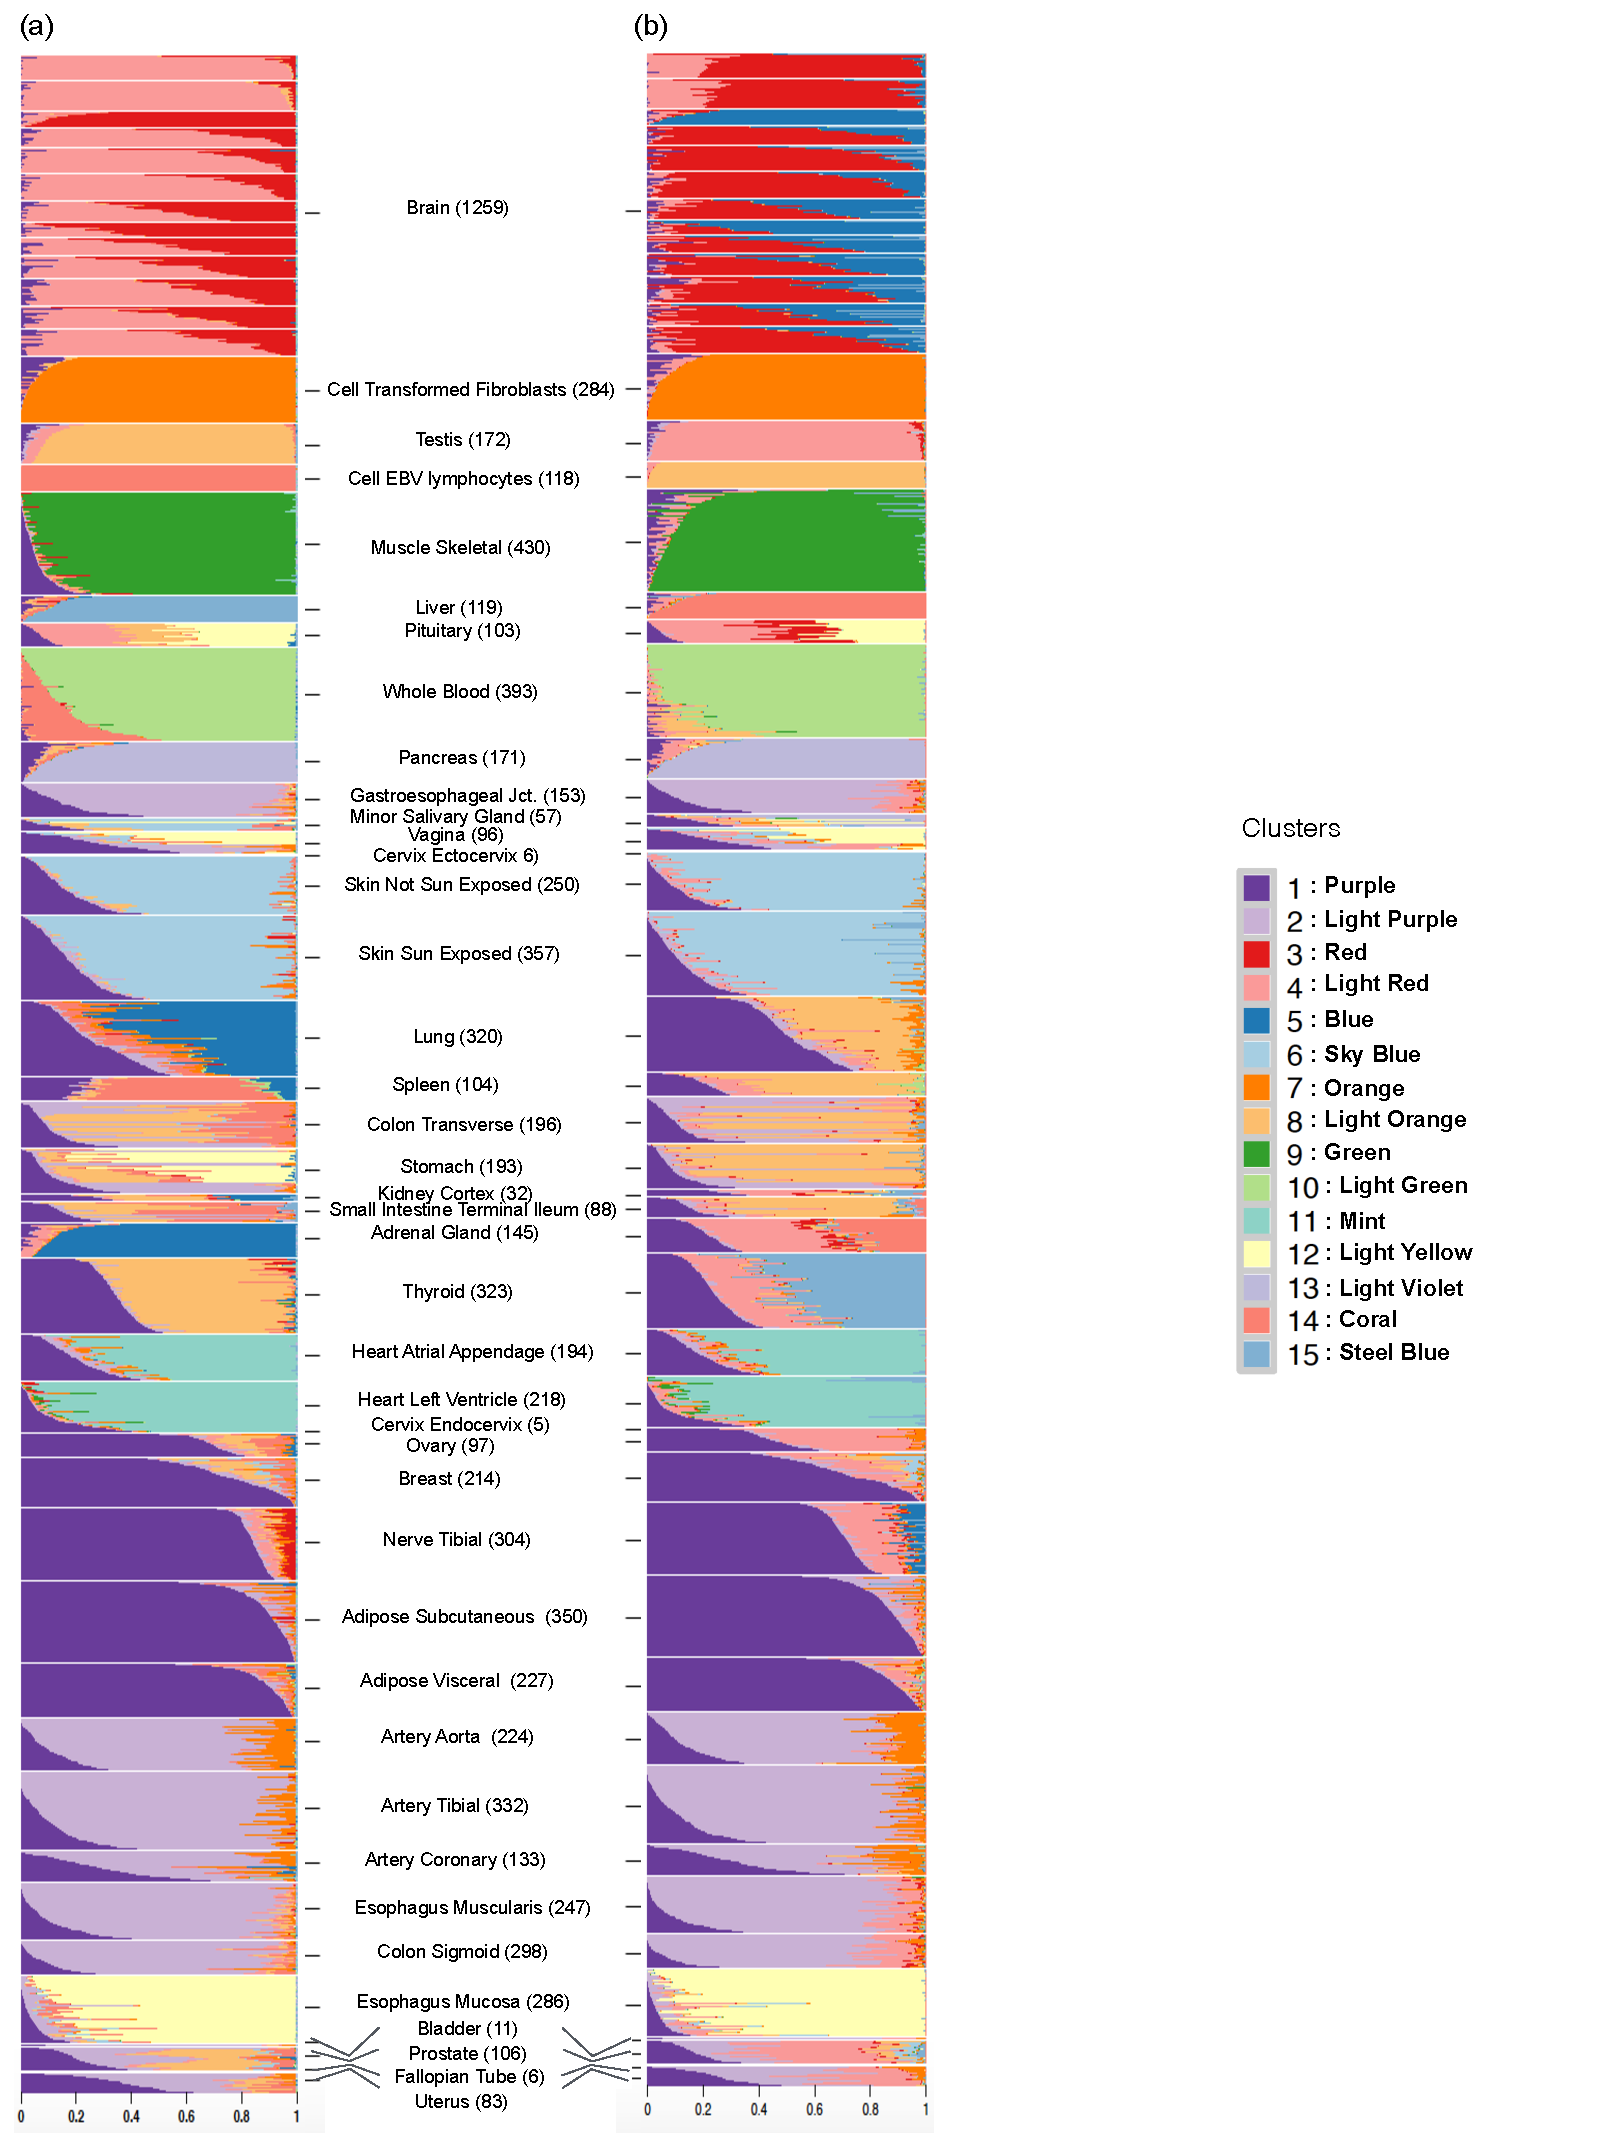
\includegraphics[height=7.5in, width=6.5in]{../plots/gtex-figures/gtex2_02_29_16.pdf}
    \caption{Structure plot of all tissue samples in 2 runs of the GTEx V6 data for  K=15 for the thinning parameters (a) $p_{thin}=0.01$ and (b) $p_{thin}=0.0001$. The patterns in two plots closely correspond to the plot in \textbf{Fig} ~\ref{fig:fig1} (a), though are a bit more noisy than compared to the unthinned version. }
 \label{fig:figS1}
    \end{figure*}

 \begin{figure*}[ht]
    \centering    
     \begin{subfigure}[t]{0.5\textwidth}
        \centering
        \includegraphics[height=2.5in]{../plots/rsz_1hierarchy_F_thin_0_01.png}
        \caption{hierarchy thin 0.01}
    \end{subfigure}%
    ~
    \begin{subfigure}[t]{0.5\textwidth}
        \centering
        \includegraphics[height=2.5in]{../plots/rsz_1admixture_F_thin_0_01.png}
        \caption{GoM thin 0.01}
    \end{subfigure}\\
    
     \begin{subfigure}[t]{0.5\textwidth}
        \centering
        \includegraphics[height=2.5in]{../plots/rsz_1hierarchy_F_thin_0_001.png}
        \caption{hierarchy 0.001}
    \end{subfigure}%
    ~
    \begin{subfigure}[t]{0.5\textwidth}
        \centering
        \includegraphics[height=2.5in]{../plots/rsz_1admixture_F_thin_0_001.png}
        \caption{GoM thin 0.001}
    \end{subfigure}\\

 \caption{A comparison of ``accuracy" of hierarchical vs model-based clustering on thinned GTEx data, with thinning parameter $p_{thin}=0.001$ and $p_{thin}=0.0001$.  For each pair of tissues from the GTEx data we assessed whether or not each clustering method (with $K=2$ clusters) separated the samples according to their actual tissue of origin, with successful separation indicated by a filled square. Thinning deteriorates accuracy compared with the unthinned data (Figure \ref{fig:fig2}), but even then the model-based method remains more successful than the hierarchical clustering in separating the samples by tissue or origin.}
 \label{fig:figS2}
\end{figure*}


\section{Supplementary Table 1}
\begin{table}[htp]
\caption{Cluster Annotations GTEx V6 data (with top gene summaries). \label{tab:supptab1}} 
\begin{center}
\begin{tabular}{|p{0.6in}|p{0.6in}|p{1.3 in}|p{3.8in}|}
\hline
Cluster & Top Driving \qquad Genes & Gene names  & Gene Summary \\
\hline
\multirow{3}{4em}{\scriptsize{cluster 1, royal purple} } &  \small{\textit{NEAT1}} & \scriptsize{nuclear paraspeckle assembly transcript 1} & \scriptsize{produces a long non-coding RNA (lncRNA) transcribed from the multiple endocrine neoplasia locus, regulates genes involved in cancer progression.}\\ 
				& \small{\textit{CCNL2}} & \scriptsize{cyclin L2} & \scriptsize{regulator of the pre-mRNA splicing process, as well as in inducing apoptosis by modulating the expression of apoptotic and antiapoptotic proteins.}\\
				& \small{\textit{SRSF5}} & \scriptsize{serine/arginine-rich splicing factor 5} & \scriptsize{encodes proteins of serine/arginine (SR)-rich family,  involved in mRNA export from the nucleus and in translation.}\\
\hline
 \multirow{3}{4em}{\scriptsize{cluster 2, light purple} } & \small{\textit{SNAP25}}  & \scriptsize{synaptosomal-associated protein, 25kDa} & \scriptsize{this gene product is a presynaptic plasma membrane protein involved in the regulation of neurotransmitter release.} \\
 					&  \small{\textit{FBXL16}}  & \scriptsize{F-box and leucine-rich repeat protein 16} & \scriptsize{members of F-box protein family, which interact with SKP1 through the F box, and they interact with ubiquitination targets through other protein interaction domains.} \\
					&  \small{\textit{SLC17A7}}  & \scriptsize{neurochondrin} & \scriptsize{encodes proteins expressed in neuron-rich regions; associated with the membranes of synaptic vesicles and functions in glutamate transport.} \\
\hline
 \multirow{3}{4em}{\scriptsize{cluster 3, red} } & \small{\textit{FABP4}}  & \scriptsize{fatty acid binding protein 4} & \scriptsize{ encodes the fatty acid binding protein found in adipocytes, takes part in fatty acid uptake, transport, and metabolism.} \\
 					&  \small{\textit{PLIN1}}  & \scriptsize{perilipin 1} & \scriptsize{protein encoded by this gene coats lipid storage droplets in adipocytes, thereby protecting them until they can be broken down by hormone-sensitive lipase.} \\
					&  \small{\textit{FASN}}  & \scriptsize{fatty acid synthase} & \scriptsize{catalyze the synthesis of palmitate from acetyl-CoA and malonyl-CoA, in the presence of NADPH, into long-chain saturated fatty acids.} \\
\hline
 \multirow{3}{4em}{\scriptsize{cluster 4, salmon} } & \small{\textit{ACTG2}}  & \scriptsize{actin, gamma 2, smooth muscle, enteric} & \scriptsize{  involved in various types of cell motility and in the maintenance of the cytoskeleton.} \\
 					&  \small{\textit{MYH11}}  & \scriptsize{myosin, heavy chain 11, smooth muscle} & \scriptsize{protein encoded by this gene is a smooth muscle myosin belonging to the myosin heavy chain family, functions as a major contractile protein, converting chemical energy into mechanical energy through the hydrolysis of ATP.} \\
					&  \small{\textit{SYNM}}  & \scriptsize{synemin} & \scriptsize{protein has been found to form a linkage between desmin, which is a subunit of the IF network, and the extracellular matrix, and provides an important structural support in muscle.} \\		
\hline
 \multirow{3}{4em}{\scriptsize{cluster 5, denim} } & \small{\textit{RGS5}}  & \scriptsize{regulator of G-protein signaling 5} & \scriptsize{encodes a member of the regulators of G protein signaling (RGS) family, associated with retinal arterial macroaneurysm.} \\
 					&  \small{\textit{MFGE8}}  & \scriptsize{milk fat globule-EGF factor 8 protein} & \scriptsize{encodes a preproprotein that is proteolytically processed to form multiple protein products, been implicated in wound healing, autoimmune disease, and cancer} \\
					&  \small{\textit{ITGA8}}  & \scriptsize{synemin} & \scriptsize{Proteins generated mediate numerous cellular processes including cell adhesion, cytoskeletal rearrangement, and activation of cell signaling pathways.} \\			\hline
 \multirow{3}{4em}{\scriptsize{cluster 6, light denim} } & \small{\textit{KRT10}}  & \scriptsize{keratin 10} & \scriptsize{encodes a member of the type I (acidic) cytokeratin family, mutations associated with epidermolytic hyperkeratosis.} \\
 					 &  \small{\textit{KRT1}} & \scriptsize{keratin 1, type II} & \scriptsize{specifically expressed in the spinous and granular layers of the epidermis with family member KRT10 and mutations in these genes have been associated with bullous congenital ichthyosiform erythroderma.} \\
					& \small{\textit{KRT2}} & \scriptsize{keratin 2, type II} & \scriptsize{expressed largely in the upper spinous layer of epidermal keratinocytes and mutations in this gene have been associated with bullous congenital ichthyosiform erythroderma.}\\
\hline
 \multirow{3}{4em}{\scriptsize{cluster 7, orange} } & \small{\textit{NEB}} & \scriptsize{nebulin} & \scriptsize{encodes nebulin, a giant protein component of the cytoskeletal matrix that coexists with the thick and thin filaments within the sarcomeres of skeletal muscle, associated with recessive nemaline myopathy.}  \\
 					 & \small{\textit{MYH1}} & \scriptsize{myosin, heavy chain 1, skeletal muscle, adult }& \scriptsize{a major contractile protein which converts chemical energy into mechanical energy through the hydrolysis of ATP.} \\
					& \small{\textit{MYH2}} & \scriptsize{myosin, heavy chain 2, skeletal muscle, adult} & \scriptsize{encodes a member of the class II or conventional myosin heavy chains, and functions in skeletal muscle contraction.} \\
\hline
\end{tabular}
\end{center}
\end{table}

\newpage



\begin{tabular}{|p{0.6in}|p{0.6in}|p{1.3 in}|p{3.8in}|}
\hline
Cluster & Top Driving \qquad Genes & Gene namese  & Gene Summary \\
\hline
 \multirow{3}{4em}{\scriptsize{cluster 8, light orange} } & \small{\textit{FN1}}  & \scriptsize{fibronectin 1} & \scriptsize{Fibronectin is involved in cell adhesion, embryogenesis, blood coagulation, host defense, and metastasis.}   \\
 					 & \small{\textit{COL1A1}} & \scriptsize{collagen, type I, alpha 1} & \scriptsize{Mutations in this gene associated with osteogenesis imperfecta types I-IV, Ehlers-Danlos syndrome type and Classical type, Caffey Disease}. \\
					      & \small{\textit{COL1A2}} & \scriptsize{collagen, type I, alpha 2} & \scriptsize{Mutations in this gene associated with osteogenesis imperfecta types I-IV, Ehlers-Danlos syndrome type and Classical type, Caffey Disease}. \\
\hline
 \multirow{3}{4em}{\scriptsize{cluster 9, green} } & \small{\textit{MBP}} & \scriptsize{myelin basic protein} & \scriptsize{major constituent of the myelin sheath of oligodendrocytes and Schwann cells in the nervous system}    \\
 					 & \small{\textit{GFAP}} & \scriptsize{glial fibrillary acidic protein} & \scriptsize{encodes one of the major intermediate filament proteins of mature astrocytes, mutations casuses Alexander disease.} \\
					      & \small{\textit{CARNS1}} & \scriptsize{carnosine synthase 1} & \scriptsize{catalyzes the formation of carnosine and homocarnosine, which are found mainly in skeletal muscle and the central nervous system, respectively}. \\
\hline
 \multirow{3}{4em}{\scriptsize{cluster 10, light green} } & \small{\textit{CYP17A1}} & \scriptsize{cytochrome P450 family 17 subfamily A member 1} & \scriptsize{encodes a member of the cytochrome P450 superfamily of enzymes, mutations in this gene are associated with isolated steroid-17 alpha-hydroxylase deficiency,20-lyase deficiency, pseudohermaphroditism, and adrenal hyperplasia.}    \\
 					 & \small{\textit{CYP11B1}} & \scriptsize{cytochrome P450 family 11 subfamily B member 1} & \scriptsize{The protein encoded by this gene plays a key role in the acute regulation of steroid hormone synthesis by enhancing the conversion of cholesterol into pregnenolone, associated with congenital lipoid adrenal hyperplasia.} \\
					      & \small{\textit{GKN1}} & \scriptsize{gastrokine 1} & \scriptsize{protein encoded by this gene is found to be down-regulated in human gastric cancer tissue as compared to normal gastric mucosa.}. \\
\hline
\multirow{3}{4em}{\scriptsize{cluster 11, turquoise} } & \small{\textit{MPZ}} & \scriptsize{myelin protein zero} & \scriptsize{specifically expressed in Schwann cells of the peripheral nervous system and encodes a type I transmembrane glycoprotein that is a major structural protein of the peripheral myelin sheath, mutations  associated with autosomal dominant form of Charcot-Marie-Tooth disease type 1 and other polyneuropathies.}    \\
 					 & \small{\textit{APOD}} & \scriptsize{apolipoprotein D} & \scriptsize{encodes a component of high density lipoprotein that has no marked similarity to other apolipoprotein sequences, closely associated with lipoprotein metabolism.} \\
					      & \small{\textit{PMP22}} & \scriptsize{peripheral myelin protein 22} & \scriptsize{encodes an integral membrane protein that is a major component of myelin in the peripheral nervous system.}. \\
\hline
\multirow{3}{4em}{\scriptsize{cluster 12, yellow} } & \small{\textit{IGHM}} & \scriptsize{immunoglobulin heavy constant mu} & \scriptsize{IgM antibodies play an important role in primary defense mechanisms, Diseases associated with IGHM include agammaglobulinemia 1 and immunodeficiency 23.}    \\
 					 & \small{\textit{IGHG1}} & \scriptsize{immunoglobulin heavy constant gamma 1 (G1m marker)} & \scriptsize{antigen binding functionality, diseases associated with IGHG1 include heavy chain deposition disease and chronic lymphocytic leukemia.} \\
					      & \small{\textit{IGHG2}} & \scriptsize{immunoglobulin heavy constant gamma 2 (G2m marker)} & \scriptsize{antigen binding gene, diseases associated with IGHG2 include c2 deficiency}. \\
\hline
\multirow{3}{4em}{\scriptsize{cluster 13, sky blue} } & \small{\textit{TG}} & \scriptsize{thyroglobulin} & \scriptsize{thyroglobulin produced predominantly in thyroid gland, synthesizes thyroxine and triiodothyronine, associated with Graves disease and Hashimotot thyroiditis.} \\
 					 &  \small{\textit{PRL}} & \scriptsize{prolactin 2} & \scriptsize{encodes the anterior pituitary hormone prolactin. This secreted hormone is a growth regulator for many tissues, including cells of the immune system.}  \\
					      & \small{\textit{PRM2}} & \scriptsize{protamine 2} & \scriptsize{Protamines are the major DNA-binding proteins in the nucleus of sperm}. \\
\hline
\multirow{3}{4em}{\scriptsize{cluster 14, light pink} } & \small{\textit{NPPA}} & \scriptsize{natriuretic peptide A} & \scriptsize{protein encoded by this gene belongs to the natriuretic peptide family, controls extracellular fluid volume and electrolyte homeostasis, mutations Mutations associated with atrial fibrillation familial type 6.} \\
 					 &  \small{\textit{MYH6}} & \scriptsize{myosin, heavy chain 6, cardiac muscle, alpha} & \scriptsize{encodes the alpha heavy chain subunit of cardiac myosin,  mutations cause familial hypertrophic cardiomyopathy and atrial septal defect 3}  \\
					      & \small{\textit{TNNT2}} & \scriptsize{protamine 2} & \scriptsize{protein encoded by this gene is the tropomyosin-binding subunit of the troponin complex, mutations in this gene have been associated with familial hypertrophic cardiomyopathy as well as with dilated cardiomyopathy}. \\
\hline
\end{tabular}

\newpage

\begin{tabular}{|p{0.6in}|p{0.6in}|p{1.3 in}|p{3.8in}|}
\hline
Cluster & Top Driving \qquad Genes & Gene namese  & Gene Summary \\
\hline
\multirow{3}{4em}{\scriptsize{cluster 15, light gray} } &  \small{\textit{KRT13}} & \scriptsize{keratin 13, type I} & \scriptsize{protein encoded by this gene is a member of the keratin gene family, associated with the autosomal dominant disorder White Sponge Nevus.}\\
 					 &  \small{\textit{KRT4}} & \scriptsize{keratin 4, type II} & \scriptsize{protein encoded by this gene is a member of the keratin gene family, associated with White Sponge Nevus, characterized by oral, esophageal, and anal leukoplakia.} \\
					      &  \small{\textit{CRNN}} & \scriptsize{cornulin} & \scriptsize{may play a role in the mucosal/epithelial immune response and epidermal differentiation. } \\
\hline
\multirow{3}{4em}{\scriptsize{cluster 16, gray} } & \small{\textit{SFTPB}} & \scriptsize{surfactant protein B} & \scriptsize {an amphipathic surfactant protein essential for lung function and homeostasis after birth, muttaions cause pulmonary alveolar proteinosis, fatal respiratory distress in the neonatal period.} \\
 					    & \small{\textit{SFTPA2}} & \scriptsize{surfactant protein A2} & \scriptsize{Mutations in this gene and a highly similar gene located nearby, which affect the highly conserved carbohydrate recognition domain, are associated with idiopathic pulmonary fibrosis.} \\
					    & \small{\textit{SFTPA1}} & \scriptsize{surfactant protein A1} &  \scriptsize{encodes a lung surfactant protein that is a member of C-type lectins called collectins, associated with idiopathic pulmonary fibrosis.} \\
\hline
\multirow{3}{4em}{\scriptsize{cluster 17, brown} } & \small{\textit{CSF3R}} & \scriptsize{colony stimulating factor 3 receptor} & \scriptsize {protein encoded by this gene is the receptor for colony stimulating factor 3, a cytokine that controls the production, differentiation, and function of granulocytes, mutations a cause of Kostmann syndrome} \\
 					    & \small{\textit{MMP25}} & \scriptsize{matrix metallopeptidase 25} & \scriptsize{proteins are involved in the breakdown of extracellular matrix in normal physiological processes, such as embryonic development, reproduction, and tissue remodeling, as well as in disease processes, such as arthritis and metastasis.} \\
					    & \small{\textit{IL1R2}} & \scriptsize{interleukin 1 receptor type 2} &  \scriptsize{protein encoded by this gene is a cytokine receptor that belongs to the interleukin 1 receptor family.} \\
\hline
\multirow{3}{4em}{\scriptsize{cluster 18, purple} } &  \small{\textit{PRSS1}} & \scriptsize{protease, serine 1} & \scriptsize{secreted by pancreas, associated with pancreatitis}\\
 					      &  \small{\textit{CPA1}} & \scriptsize{carboxypeptidase A1} & \scriptsize{secreted by pancreas, linked to pancreatitis and pancreatic cancer} \\
					      &  \small{\textit{PNLIP}} & \scriptsize{pancreatic lipase} & \scriptsize{encodes a carboxyl esterase that hydrolyzes insoluble, emulsified triglycerides, and is essential for the efficient digestion of dietary fats. This gene is expressed specifically in the pancreas.}\\
\hline
\multirow{3}{4em}{\scriptsize{cluster 19, pink} } & \small{\textit{HBB}} & \scriptsize{hemoglobin, beta} & \scriptsize{mutant beta globin causes sickle cell anemia, absence of beta chain/ reduction in beta globin leads to thalassemia.}\\
 					      & \small{\textit{HBA2}} & \scriptsize{hemoglobin, alpha 2} & \scriptsize{deletion of alpha genes may lead to alpha thalassemia.}  \\
					      & \small{\textit{HBA1}} & \scriptsize{hemoglobin, alpha 1} & \scriptsize{deletion of alpha genes may lead to alpha thalassemia.}  \\
\hline
\multirow{3}{4em}{\scriptsize{cluster 20, dark gray} } &  \small{\textit{ALB}} & \scriptsize{albumin} & \scriptsize{functions primarily as a carrier protein for steroids, fatty acids, and thyroid hormones and plays a role in stabilizing extracellular fluid volume.} \\
					      &  \small{\textit{HP}} & \scriptsize{haptoglobin} & \scriptsize{encodes a preproprotein, which subsequently  produces haptoglobin, linked to diabetic nephropathy, Crohn's disease, inflammatory disease behavior and reduced incidence of Plasmodium falciparum malaria.}\\
					      & \small{\textit{FGB}} & \scriptsize{fibrinogen beta chain} & \scriptsize{protein encoded by this gene is the beta component of fibrinogen, mutations may lead to several disorders, including afibrinogenemia, dysfibrinogenemia, hypodysfibrinogenemia etc.}  \\
\hline
\end{tabular}

\clearpage
			
\section{Supplementary Table 2}
\begin{table}[htp]
\begin{center}
\caption{Cluster Annotations GTEx V6 Brain data (with top gene summaries).\label{tab:supptab2}}
\begin{tabular}{|p{0.7in}|p{0.7in}|p{1.4in}|p{3.6in}|} 
\hline
Cluster & Top Driving \qquad Genes & Gene names & Gene Summary \\
\hline
 \multirow{3}{4em}{\small{cluster 1, royal blue}}  &  \small{\textit{CLU}} &  \footnotesize{clusterin} & \scriptsize{protein encoded by this gene is a secreted chaperone that can under some stress conditions also be found in the cell cytosol, also involved in cell death, tumor progression, and neurodegenerative disorders.} \\ 
 					      & \small{\textit{OXT}} &  \footnotesize{oxytocin/neurophysin I prepropeptide} & \scriptsize{encodes a precursor protein that is processed to produce oxytocin and neurophysin I, involved in contraction of  smooth muscle during parturition and lactation, cognition, tolerance, adaptation and complex sexual and maternal behaviour.} \\ 
					      & \small{\textit{GLUL}} & \footnotesize{glutamate-ammonia ligase} & \scriptsize{catalyzes the synthesis of glutamine from glutamate and ammonia in an ATP-dependent reaction,  associated with congenital glutamine deficiency, and overexpression of this gene was observed in some primary liver cancer samples.} \\
\hline
 \multirow{3}{4em}{\small{cluster 2, turquoise}}  & \small{\textit{ENC1}} & \footnotesize{ectodermal-neural cortex 1} & \scriptsize{plays a role in the oxidative stress response as a regulator of the transcription factor Nrf2, may play role in malignant transformation.} \\
 							&  \small{\textit{NCALD}} & \footnotesize{neurocalcin delta} & \scriptsize{ encodes a member of the neuronal calcium sensor (NCS), a regulator of G protein-coupled receptor signal transduction.}   \\ 
 					      & \small{\textit{YWHAH}} &  \footnotesize{tyrosine 3-monooxygenase/tryptophan 5-monooxygenase activation protein eta} & \scriptsize{mediate signal transduction by binding to phosphoserine-containing proteins, associated with early-onset schizophrenia and psychotic bipolar disorder.} \\
\hline
 \multirow{3}{4em}{\small{cluster 3, lime green}} & \small{\textit{PKD1}} & \footnotesize{polycystin 1, transient receptor potential channel interacting} & \scriptsize{functions as a regulator of calcium permeable cation channels and intracellular calcium homoeostasis. It is also involved in cell-cell/matrix interactions and may modulate G-protein-coupled signal-transduction pathways.}\\
 					    & \small{\textit{CBLN3}} & \footnotesize{cerebellin 3 precursor} & \scriptsize{ contain a cerebellin motif and C-terminal C1q signature domain that mediates trimeric assembly of atypical collagen complexes} \\
					    &  \small{\textit{CHGB}} &  \footnotesize{chromogranin B} & \scriptsize{ encodes a tyrosine-sulfated secretory protein abundant in peptidergic endocrine cells and neurons. This protein may serve as a precursor for regulatory peptides.} \\
 \hline
  \multirow{3}{4em}{\small{cluster 4, red}} & \small{\textit{PPP1R1B}} & \footnotesize{protein phosphatase 1 regulatory inhibitor sub-
unit 1B} & \scriptsize{encodes a bifunctional signal transduction molecule, may serve as a therapeutic target for neurologic and psychiatric disorders.}\\
 					    & \small{\textit{RGS14}} & \footnotesize{regulator of G-protein signaling 14} & \scriptsize{ attenuates the signaling activity of G-proteins, increases the rate of conversion of the GTP to GDP.} \\
					    &  \small{\textit{NCDN}} &  \footnotesize{neurochondrin} & \scriptsize{ encodes a leucine-rich cytoplasmic protein, essential for spatial learning processes.} \\
 \hline
 \multirow{3}{4em}{\small{cluster 5,  yellow orange}} & \small{\textit{MBP}} & \footnotesize{myelin basic protein} & \scriptsize{protein encoded is a major constituent of the myelin sheath of oligodendrocytes and Schwann cells in the nervous system.} \\
 					    & \small{\textit{GFAP}} & \footnotesize{glial fibrillary acidic protein} & \scriptsize{ encodes major intermediate filament proteins of mature astrocytes, a marker to distinguish astrocytes during development, mutations in this gene cause Alexander disease, a rare disorder of astrocytes in central nervous system.} \\
					    & \small{\textit{TF}}  & \footnotesize{transferrin}  & \scriptsize{transport iron from the intestine, reticuloendothelial system, and liver parenchymal cells to all proliferating cells in the body, involved in the removal of certain organic matter and allergens from serum.}\\
\hline
 \multirow{3}{4em}{\small{cluster 6,  yellow}} & \small{\textit{IQGAP1}} & \footnotesize{IQ motif containing GTPase activating protein 1} & \scriptsize{interacts with components of the cytoskeleton, with cell adhesion molecules, and with several signaling molecules to regulate cell morphology and motility.} \\
 					    & \small{\textit{A2M}} & \footnotesize{alpha-2-macroglobulin} & \scriptsize{ inhibits many proteases, including trypsin, thrombin and collagenase. A2M is implicated in Alzheimer disease (AD) due to its ability to mediate the clearance and degradation of A-beta, the major component of beta-amyloid deposits.} \\
					    & \small{\textit{C3}}  & \footnotesize{complement component 3}  & \scriptsize{plays a central role in the activation of complement system, associated with atypical hemolytic uremic syndrome and age-related macular degeneration in human patients.}\\
\hline
\end{tabular}
 \end{center} 
\end{table}

\clearpage


\clearpage
\paragraph*{S3 Table.}
\label{supptab3}
{\bf Deng et al (2014) Cluster 1 (blue) top GO annotations.}

\begin{table}[!hp]
\begin{adjustwidth}{-.5in}{0in}
\begin{tabular}{|c|c|p{1.5in}|p{4in}|}
  \hline
 & go.id & name & significant \\ 
  \hline
1 & GO:0007276 & gamete generation & \footnotesize{BCL2L10; GDF9; NOBOX; PABPC1L; RGS2; CREB3L4; RNF114; BMP15; PTTG1; TDRD12; WEE2; SPIN1; DAZL} \\ 
  2 & GO:0007292 & female gamete generation & \footnotesize{GDF9; BCL2L10; PABPC1L; BMP15; WEE2; DAZL; NOBOX} \\ 
  3 & GO:0048609 & multicellular organismal reproductive process & \footnotesize{GDF9; NOBOX; PABPC1L; BCL2L10; BMP15; CREB3L4; TGFB2; RNF114; RGS2; PTTG1; TDRD12; WEE2; SPIN1; DAZL} \\ 
  4 & GO:0032504 & multicellular organism reproduction & \footnotesize{GDF9; NOBOX; PABPC1L; BCL2L10; BMP15; CREB3L4; TGFB2; RNF114; RGS2; PTTG1; TDRD12; WEE2; SPIN1; DAZL}\\ 
  5 & GO:0019953 & sexual reproduction & \footnotesize{BCL2L10; GDF9; NOBOX; PABPC1L; RGS2; CREB3L4; RNF114; BMP15; PTTG1; TDRD12; WEE2; SPIN1; DAZL} \\ 
  6 & GO:0044702 & single organism reproductive process & \footnotesize{GDF9; NOBOX; PABPC1L; BCL2L10; BMP15; CREB3L4; TGFB2; CASP8; RNF114; RGS2; PTTG1; TDRD12; WEE2; SPIN1; DAZL} \\ 
  7 & GO:0048477 & oogenesis & \footnotesize{WEE2; GDF9; NOBOX; PABPC1L; DAZL} \\ 
  8 & GO:0044703 & multi-organism reproductive process & \footnotesize{BCL2L10; GDF9; NOBOX; PABPC1L; RGS2; CREB3L4; RNF114; BMP15; PTTG1; TDRD12; WEE2; SPIN1; DAZL} \\ 
  9 & GO:0048599 & oocyte development  & \footnotesize{WEE2; GDF9; PABPC1L; DAZL} \\ 
  10 & GO:0009994 & oocyte differentiation & \footnotesize{WEE2; GDF9; PABPC1L; DAZL} \\ 
  11 & GO:0051321 & meiotic cell cycle & \footnotesize{H1FOO; WEE2; TDRD12; SPIN1; PTTG1; DAZL} \\ 
  12 & GO:0001556 & oocyte maturation & \footnotesize{WEE2; PABPC1L; DAZL} \\ 
  13 & GO:0006306 & DNA methylation & \footnotesize{TDRD12; H1FOO; TET3; ZFP57} \\ 
  14 & GO:0051302 & regulation of cell division & \footnotesize{TGFB2; PTTG1; TXNIP; WEE2; CHEK1; DAZL} \\ 
  15 & GO:0060255 & regulation of macromolecule metabolic process & \footnotesize{TGFB2; NOBOX; BPGM; UBE2D3; NFYA; CASP8; BMP15; TXNIP; TDRD12; GDF9; BCL2L10} \\ 
 \hline
\end{tabular}
\end{adjustwidth}
\end{table}


\paragraph*{S3 Table continued.}
{\bf Deng et al (2014) Cluster 2 (magenta) top GO annotations.}

\begin{table}[!hp]
\begin{adjustwidth}{-.5in}{0in}
\begin{tabular}{|c|c|p{1.5in}|p{4in}|}
  \hline
 & go.id & name  & significant \\ 
  \hline
1 & GO:0016604 & nuclear body  & \footnotesize{YTHDC1; RBM8A; CDK12; PSME4; PPP1R8; HIPK1; TOPORS} \\ 
  2 & GO:0005814 & centriole  & \footnotesize{SFI1; PLK2; ROCK1; TOPORS} \\ 
  3 & GO:0044450 & microtubule organizing center part  & \footnotesize{SFI1; PLK2; ROCK1; TOPORS} \\ 
   \hline
\end{tabular}
 \end{adjustwidth} 
  \end{table}


\clearpage
\paragraph*{S3 Table continued.}
{\bf Deng et al (2014) Cluster 3 (yellow) top GO annotations.}

\begin{table}[!hp]
\begin{adjustwidth}{-.5in}{0in}
\begin{tabular}{|c|c|p{1.5in}|p{4in}|}
  \hline
 & go.id & name  & significant \\ 
  \hline
1 & GO:0044428 & nuclear part  & \footnotesize{MAD2L2; SMARCC1; PPRC1; SLU7; NFYB; TOR1B; MIOS; NR1H3; POLR3K} \\ 
  2 & GO:0031981 & nuclear lumen & \footnotesize{MAD2L2; SMARCC1; PPRC1; SLU7; NFYB; POLR1E; MIOS; POLR3K; XPO1}\\ 
  3 & GO:0070013 & intracellular organelle lumen & \footnotesize{MAD2L2; SMARCC1; PPRC1; SLU7; NFYB; POLR1E; MIOS; POLR3K; XPO1; DNTTIP2; ZBTB10; ZBTB17} \\ 
  4 & GO:0043233 & organelle lumen & \footnotesize{MAD2L2; SMARCC1; PPRC1; SLU7; NFYB; POLR1E; MIOS; POLR3K; XPO1} \\ 
  5 & GO:0005730 & nucleolus & \footnotesize{XPO1; DNTTIP2; ESF1; WDR43; ZDHHC7; HEATR1; POLR1E; DDX24; POLR3K} \\ 
  6 & GO:0005634 & nucleus & \footnotesize{MAD2L2; SMARCC1; PPRC1; SLU7; NFYB; TOR1B; MIOS; NR1H3; EIF5B; POLR3K} \\ 
  7 & GO:0044446 & intracellular organelle part & \footnotesize{MAD2L2; PTDSS2; SMARCC1; KLHL21; TOR1B; PPRC1; SLU7; NFYB; SLC25A36; ECE2} \\ 
  8 & GO:0005654 & nucleoplasm & \footnotesize{MAD2L2; SMARCC1; PPRC1; SLU7; NFYB; POLR1E; MIOS; POLR3K; XPO1; ZBTB10; ZBTB17} \\ 
  9 & GO:0003723 & RNA binding & \footnotesize{PPRC1; EIF5B; XPO1; DNTTIP2; WDR43; DDX10; EIF3C; BCLAF1; EBNA1BP2; RARS}\\ 
  10 & GO:0003676 & nucleic acid binding & \footnotesize{SMARCC1; PPRC1; SLU7; NFYB; POLR1E; EIF5B; POLR3K; XPO1; DNTTIP2} \\ 
  11 & GO:0043231 & intracellular membrane-bounded organelle &  \footnotesize{MAD2L2; PTDSS2; SMARCC1; TOR1B; PPRC1; SLU7; NFYB; ESF1; ECE2; LMAN1L} \\ 
  12 & GO:0043229 & intracellular organelle & \footnotesize{MAD2L2; PTDSS2; SMARCC1; KLHL21; TOR1B; PPRC1; ARRDC1; SLU7; NFYB; ESF1; ECE2} \\ 
  13 & GO:0005874 & microtubule & \footnotesize{WDR43; KLHL21; HAUS6; CENPE; TEKT2; RACGAP1; WDR81; BCL2L11; KIF20B} \\ 
  14 & GO:0044822 & poly(A) RNA binding & \footnotesize{WDR43; DNTTIP2; ESF1; NXF1; DDX10; HEATR1; EIF3C} \\ 
  15 & GO:0044424 & intracellular part & \footnotesize{MAD2L2; PTDSS2; SMARCC1; KLHL21; TOR1B; PPRC1; SNAPC4; POLR3K; ARRDC1; SLU7; NFYB; ESF1; WDR43; ECE2; LMAN1L} \\ 
%  16 & GO:0043228 & non-membrane-bounded organelle & c & 3207 & MAD2L2; SMARCC1; KLHL21; WDR81; POLR3K; XPO1; DNTTIP2; WDR43; BCL2L11; YPEL2; HAUS6; TEKT2; BCLAF1; NF2; URB2; NR1H3; ESF1; HEATR1; CENPE; EIF4E; USP33; EBNA1BP2; PAFAH1B2; NASP; ZDHHC7; DDX24; TRAIP; RACGAP1; WDR36; POLRMT; ATXN7; KIF20B; KDM5A; POLR1E \\ 
%  17 & GO:0043232 & intracellular non-membrane-bounded organelle & c & 3207 & MAD2L2; SMARCC1; KLHL21; WDR81; POLR3K; XPO1; DNTTIP2; WDR43; BCL2L11; YPEL2; HAUS6; TEKT2; BCLAF1; NF2; URB2; NR1H3; ESF1; HEATR1; CENPE; EIF4E; USP33; EBNA1BP2; PAFAH1B2; NASP; ZDHHC7; DDX24; TRAIP; RACGAP1; WDR36; POLRMT; ATXN7; KIF20B; KDM5A; POLR1E \\ 
%  18 & GO:0051233 & spindle midzone & c &  23 & RACGAP1; CENPE; KIF20B \\ 
%  19 & GO:0003847 & 1-alkyl-2-acetylglycerophosphocholine esterase activity & m &   5 & ASPG; PAFAH1B2 \\ 
%  20 & GO:1990023 & mitotic spindle midzone & c &   5 & CENPE; KIF20B \\ 
%  21 & GO:0008017 & microtubule binding & m & 169 & WDR43; BCL2L11; RACGAP1; CENPE; WDR81; KIF20B \\ 
%  22 & GO:0071014 & post-mRNA release spliceosomal complex & c &   6 & CRNKL1; TFIP11 \\ 
%  23 & GO:1901363 & heterocyclic compound binding & m & 4675 & SMARCC1; PPRC1; POLR3K; TFIP11; NFYB; TOR1B; EIF5B; CHKA; XPO1; DNTTIP2; ZBTB10; ZBTB17; DDX10; EIF3C; BCLAF1; CRNKL1; RARS; ITPKC; RANBP2; ESF1; NXF1; HEATR1; CENPE; SNUPN; PRKCD; SPIC; WDR43; SNAPC4; EIF4E; EBNA1BP2; UBR5; THAP4; SOS1; DDX24; PFKFB3; SLU7; GEMIN5; WDR36; POLRMT; NR1H3; KIF20B; KDM5A; POLR1E \\ 
%  24 & GO:0043227 & membrane-bounded organelle & c & 9724 & MAD2L2; PTDSS2; SMARCC1; TOR1B; PPRC1; SNAPC4; SLU7; NFYB; ESF1; ECE2; LMAN1L; MIOS; NR1H3; EIF5B; POLR3K; XPO1; DNTTIP2; ZBTB10; ZBTB17; NOB1; TFIP11; HAUS6; TEKT2; BCLAF1; CRNKL1; RARS; SLC25A36; NF2; CTNNBL1; URB2; MGEA5; RANBP2; POLR1E; ITPKC; SNUPN; CTSL; NXF1; HEATR1; CENPE; CTSC; NPC1L1; ATP1B3; RTN2; PRKCD; SPIC; TNIP1; LAMP2; GFPT1; EIF4E; BCL2L11; USP33; EBNA1BP2; UBR5; PAFAH1B2; GINS3; NASP; WDR43; ZDHHC7; DDX24; RACGAP1; PFKFB3; YPEL2; TRAIP; GEMIN5; SLC9A9; WDR36; POLRMT; ATXN7; RNF216; KIF20B; KDM5A; ARRDC1 \\ 
%  25 & GO:0097159 & organic cyclic compound binding & m & 4744 & SMARCC1; PPRC1; POLR3K; TFIP11; NFYB; TOR1B; EIF5B; CHKA; XPO1; DNTTIP2; ZBTB10; ZBTB17; DDX10; EIF3C; BCLAF1; CRNKL1; RARS; ITPKC; RANBP2; ESF1; NXF1; HEATR1; CENPE; SNUPN; PRKCD; SPIC; WDR43; SNAPC4; EIF4E; EBNA1BP2; UBR5; THAP4; SOS1; DDX24; PFKFB3; SLU7; GEMIN5; WDR36; POLRMT; NR1H3; KIF20B; KDM5A; POLR1E \\ 
%  26 & GO:0005622 & intracellular & c & 11307 & MAD2L2; PTDSS2; SMARCC1; KLHL21; TOR1B; PPRC1; SNAPC4; POLR3K; ARRDC1; SLU7; NFYB; ESF1; WDR43; ECE2; LMAN1L; MIOS; NASP; NR1H3; EIF5B; CHKA; XPO1; DNTTIP2; ZBTB10; ZBTB17; NOB1; TFIP11; HAUS6; EIF3C; BCLAF1; CRNKL1; ATG3; RARS; SLC25A36; NF2; CTNNBL1; URB2; MGEA5; RANBP2; POLR1E; ITPKC; SNUPN; CTSL; NXF1; HEATR1; CENPE; CTSC; NPC1L1; ATP1B3; RTN2; PRKCD; SPIC; TNIP1; LAMP2; ATXN7; EIF4E; BCL2L11; USP33; EBNA1BP2; UBR5; PAFAH1B2; GINS3; DPH2; ZDHHC7; SOS1; DDX24; RACGAP1; PFKFB3; YPEL2; TRAIP; GEMIN5; SLC9A9; WDR36; TEKT2; POLRMT; GFPT1; RNF216; KIF20B; KDM5A; WDR81 \\ 
%  27 & GO:0043234 & protein complex & c & 3677 & MAD2L2; SMARCC1; KLHL21; NFYB; WDR81; MIOS; POLR3K; XPO1; WDR43; BCL2L11; HAUS6; EIF3C; ATG3; RARS; NF2; CTNNBL1; RANBP2; NXF1; HEATR1; CENPE; ATP1B3; SNAPC4; EIF4E; USP33; CRNKL1; NASP; GEMIN5; RACGAP1; WDR36; TEKT2; ATXN7; NR1H3; KIF20B; KDM5A; POLR1E \\ 
%  28 & GO:0000339 & RNA cap binding & m &  10 & EIF4E; SNUPN \\ 
%  29 & GO:0034062 & RNA polymerase activity & m &  40 & POLRMT; POLR3K; POLR1E \\ 
%  30 & GO:0072686 & mitotic spindle & c &  40 & RACGAP1; CENPE; KIF20B \\ 
\hline
\end{tabular}
\end{adjustwidth} 
  \end{table}


\clearpage
\paragraph*{S3 Table continued.}
{\bf Deng et al (2014) Cluster 4 (green) top GO annotations.}
\begin{table}[!hp]
\begin{adjustwidth}{-.5in}{0in}
\begin{tabular}{|c|c|p{1.5in}|p{4in}|}
  \hline
 & go.id & name & significant \\ 
  \hline
1 & GO:0005829 & cytosol & \footnotesize{PARG; UAP1; PSMB10; TCEB1; RPLP0; EIF5; CNBP; RPS3; PSAT1; AACS; PMM1; EXOSC7; EIF3I; SET; BHMT; BHMT2} \\ 
  2 & GO:0044444 & cytoplasmic part & \footnotesize{PARG; UAP1; PSMB10; TCEB1; HSPA8; SERINC1; EIF5; CNBP; RPS3; PSAT1; GPD2; AACS; GPR137B; STIP1; PMM1; EXOSC7; VPREB3; PEX16} \\ 
  3 & GO:0055131 & C3HC4-type RING finger domain binding & \footnotesize{HSPA8; PINK1; DNAJA1} \\ 
  4 & GO:1901575 & organic substance catabolic process & \footnotesize{PSMB10; TCEB1; RPLP0; RPS3; GPD2; PINK1; EXOSC7; ALLC; BHMT; HSP90AB1; RPL13A; ATG7; CUL5; UBXN1; ZMPSTE24} \\ 
  5 & GO:0000151 & ubiquitin ligase complex & \footnotesize{DNAJA1; RNF7; UBE2C; HSPA8; FBXO15; SUGT1; DCAF4; CUL5; FBXL20} \\ 
  6 & GO:0072655 & protein localization to mitochondrion & \footnotesize{TIMM17A; BNIP3L; ARIH2; PEMT; SFN; PINK1; HSP90AA1; TIMM23} \\ 
  7 & GO:1901564 & organonitrogen compound metabolic process & \footnotesize{PSMB10; RPLP0; SERINC1; EIF5; BHMT2; PINK1; EIF3I; ALLC; BHMT; MRPL22; RPL13A; ATG7; NUDT9; VNN1; CTSA; HK1} \\ 
  8 & GO:0005737 & cytoplasm & \footnotesize{PARG; UAP1; PSMB10; TCEB1; HSPA8; SERINC1; EIF5; CNBP; RPS3; PSAT1; GPD2; AACS; GPR137B; STIP1; PMM1; EXOSC7} \\ 
  9 & GO:0044265 & cellular macromolecule catabolic process & \footnotesize{EXOSC7; SUMO2; BNIP3L; ARIH2; PSMB10; TCEB1; RPLP0; UBXN1; HSP90AB1; RPL13A; RPS3; RNF7; PINK1} \\ 
10 & GO:0023026 & MHC class II protein complex binding & \footnotesize{HSP90AB1; HSP90AA1; HSPA8} \\ 
11 & GO:0051082 & unfolded protein binding & \footnotesize{DNAJA1; PTGES3; HSPA8; HSP90AB1; HSP90AA1; NPM1} \\ 
12 & GO:0009056 & catabolic process & \footnotesize{PSMB10; TCEB1; RPLP0; RPS3; GPD2; PINK1; EXOSC7; ALLC; WDR45; HSP90AB1; RPL13A} \\ 
13 & GO:0009057 & macromolecule catabolic process & \footnotesize{EXOSC7; SUMO2; BNIP3L; ARIH2; PSMB10; TCEB1; RPLP0; AZIN1; UBXN1; HSP90AB1; RPL13A} \\ 
14 & GO:0044248 & cellular catabolic process & \footnotesize{PSMB10; TCEB1; SUMO2; RPS3; GPD2; PINK1; EXOSC7; ALLC; WDR45; HSP90AB1} \\ 
 15 & GO:0006626 & protein targeting to mitochondrion  & \footnotesize{TIMM17A; BNIP3L; ARIH2; PEMT; PINK1; HSP90AA1; TIMM23} \\ 
%  16 & GO:0030163 & protein catabolic process & b & 705 & BNIP3L; ARIH2; PSMB10; TCEB1; SUMO2; AZIN1; UBXN1; HSP90AB1; ATG7; RNF7; PINK1; CUL5; FBXL20; UBE2C; ZMPSTE24 \\ 
%  17 & GO:0044711 & single-organism biosynthetic process & b & 1499 & MRPL22; SERINC1; CNBP; BHMT2; GPD2; PINK1; PMM1; BHMT; CITED1; ISYNA1; STAG2; UAP1; BCAT1; APRT; MRPS18B; PHGDH; FDPS; DPH3; PEMT; PTGES3; AZIN1; PSAT1; GPD1L \\ 
%  18 & GO:0033477 & S-methylmethionine metabolic process & b &   2 & BHMT2; BHMT \\ 
%  19 & GO:0033528 & S-methylmethionine cycle & b &   2 & BHMT2; BHMT \\ 
%  20 & GO:0023023 & MHC protein complex binding & m &  12 & HSP90AB1; HSP90AA1; HSPA8 \\ 
%  21 & GO:0072594 & establishment of protein localization to organelle & b & 570 & HSP90AB1; TIMM17A; BNIP3L; ARIH2; PEMT; RPLP0; SFN; RPL13A; RPS3; PINK1; HSP90AA1; TIMM23; PEX16 \\ 
%  22 & GO:0044257 & cellular protein catabolic process & b & 583 & BNIP3L; ARIH2; PSMB10; TCEB1; SUMO2; UBXN1; HSP90AB1; RNF7; PINK1; CUL5; FBXL20; UBE2C; ZMPSTE24 \\ 
%  23 & GO:0031461 & cullin-RING ubiquitin ligase complex & c & 112 & RNF7; UBE2C; FBXO15; DCAF4; CUL5; FBXL20 \\ 
%  24 & GO:0043632 & modification-dependent macromolecule catabolic process & b & 515 & ARIH2; PSMB10; TCEB1; SUMO2; UBXN1; HSP90AB1; RNF7; PINK1; CUL5; FBXL20; UBE2C; ZMPSTE24 \\ 
%  25 & GO:0009331 & glycerol-3-phosphate dehydrogenase complex & c &   3 & GPD1L; GPD2 \\ 
%  26 & GO:0044267 & cellular protein metabolic process & b & 4315 & PSMB10; TCEB1; RPLP0; EIF5; SUMO2; RPS3; PINK1; PMM1; EIF3I; SET; BHMT; MRPL22; HSP90AB1; RPL13A; ATG7; CUL5; HDGF; UBXN1; ZMPSTE24; WDR45; DPH3; HSPA8; BNIP3L; ARIH2; STAG2; CTSA; UAP1; TIMM17A; MRPS18B; GPD1L; LDB1; RNF7; NPM1; PA2G4; ALPPL2; DNAJA1; PTGES3; FBXL20; UBE2C; KNG1; SFN; DCAF4; HSP90AA1; TIMM23 \\ 
%  27 & GO:0031625 & ubiquitin protein ligase binding & m & 240 & DNAJA1; UBE2C; HSPA8; UBXN1; SUMO2; PINK1; CUL5; PA2G4 \\ 
%  28 & GO:0044389 & ubiquitin-like protein ligase binding & m & 244 & DNAJA1; UBE2C; HSPA8; UBXN1; SUMO2; PINK1; CUL5; PA2G4 \\ 
%  29 & GO:0008652 & cellular amino acid biosynthetic process & b &  82 & PSAT1; BHMT2; BHMT; BCAT1; PHGDH \\ 
%  30 & GO:0006520 & cellular amino acid metabolic process & b & 393 & BHMT; PEMT; PSMB10; SERINC1; AZIN1; BCAT1; PSAT1; BHMT2; ATG7; PHGDH \\ 
%  31 & GO:0046500 & S-adenosylmethionine metabolic process & b &  18 & BHMT2; BHMT; PEMT \\ 
%  32 & GO:0051603 & proteolysis involved in cellular protein catabolic process & b & 560 & ARIH2; PSMB10; TCEB1; SUMO2; UBXN1; HSP90AB1; RNF7; PINK1; CUL5; FBXL20; UBE2C; ZMPSTE24 \\ 
%  33 & GO:0019538 & protein metabolic process & b & 4833 & PSMB10; TCEB1; RPLP0; EIF5; SUMO2; RPS3; PINK1; PMM1; EIF3I; SET; BHMT; MRPL22; HSP90AB1; RPL13A; NAALAD2; ATG7; CUL5; HDGF; UBXN1; ZMPSTE24; WDR45; DPH3; HSPA8; BNIP3L; ARIH2; STAG2; CTSA; UAP1; TIMM17A; MRPS18B; GPD1L; LDB1; RNF7; NPM1; PA2G4; ALPPL2; DNAJA1; PEMT; PTGES3; FBXL20; UBE2C; KNG1; AZIN1; SFN; DCAF4; HSP90AA1; TIMM23 \\ 
%  34 & GO:0071806 & protein transmembrane transport & b &  47 & HSP90AA1; TIMM17A; TIMM23; PEX16 \\ 
%  35 & GO:0033365 & protein localization to organelle & b & 752 & HSP90AB1; DNAJA1; BNIP3L; ARIH2; PEMT; RPLP0; SFN; RPL13A; TIMM17A; RPS3; PINK1; HSP90AA1; TIMM23; PEX16 \\ 
%  36 & GO:0044237 & cellular metabolic process & b & 8425 & PARG; UAP1; PSMB10; TCEB1; HSPA8; SERINC1; EIF5; SUMO2; CNBP; RPS3; PSAT1; GPD2; AACS; DPH3; PMM1; EXOSC7; ISYNA1; EIF3I; SET; ALLC; BHMT; BHMT2; MRPL22; HSP90AB1; RPL13A; NAALAD2; ATG7; VNN1; CUL5; CITED1; HDGF; UBXN1; ZMPSTE24; WDR45; NUDT9; RPLP0; BNIP3L; ARIH2; FDPS; STAG2; CTSA; HK1; TIMM17A; BCAT1; GPD1L; APRT; LDB1; MRPS18B; PHGDH; RNF7; HCRT; NPM1; PA2G4; ALPPL2; ACTN2; DNAJA1; PINK1; PEMT; PTMA; PTGES3; FBXL20; UBE2C; KNG1; AZIN1; SFN; DCAF4; HSP90AA1; MTA3; TIMM23 \\ 
%  37 & GO:0044419 & interspecies interaction between organisms & b & 763 & FDPS; RPLP0; BNIP3L; PSMB10; TCEB1; HSPA8; HSP90AB1; RPL13A; SET; RPS3; ATG7; CUL5; NPM1; SUGT1 \\ 
%  38 & GO:0044403 & symbiosis, encompassing mutualism through parasitism & b & 763 & FDPS; RPLP0; BNIP3L; PSMB10; TCEB1; HSPA8; HSP90AB1; RPL13A; SET; RPS3; ATG7; CUL5; NPM1; SUGT1 \\ 
%  39 & GO:0034613 & cellular protein localization & b & 1375 & WDR45; ACTN2; DNAJA1; BNIP3L; ARIH2; PEMT; CTSA; RPLP0; TIMM23; REEP1; SFN; RPL13A; TIMM17A; RPS3; HSP90AB1; PINK1; HSP90AA1; GPD1L; NPM1; PEX16 \\ 
%  40 & GO:0070727 & cellular macromolecule localization & b & 1382 & WDR45; ACTN2; DNAJA1; BNIP3L; ARIH2; PEMT; CTSA; RPLP0; TIMM23; REEP1; SFN; RPL13A; TIMM17A; RPS3; HSP90AB1; PINK1; HSP90AA1; GPD1L; NPM1; PEX16 \\ 
%  41 & GO:0044822 & poly(A) RNA binding & m & 1066 & FDPS; RPLP0; LARP4; MRPL22; RPL13A; HSPA8; EIF5; SUMO2; HSP90AB1; CNBP; RPS3; GRN; HSP90AA1; STIP1; HDGF; NPM1; PA2G4 \\ 
%  42 & GO:0044281 & small molecule metabolic process & b & 2196 & PSMB10; HSPA8; SERINC1; CNBP; BHMT2; GPD2; AACS; VNN1; PMM1; BHMT; ATG7; NUDT9; HK1; ISYNA1; CTSA; UAP1; BCAT1; APRT; PHGDH; HSP90AA1; FDPS; PEMT; PTGES3; PINK1; AZIN1; PSAT1; GPD1L \\ 
%  43 & GO:0044283 & small molecule biosynthetic process & b & 420 & FDPS; BHMT; PEMT; PTGES3; BCAT1; PSAT1; CNBP; BHMT2; PHGDH; ISYNA1 \\ 
%  44 & GO:0071704 & organic substance metabolic process & b & 8704 & PARG; UAP1; PSMB10; TCEB1; HSPA8; SERINC1; EIF5; SUMO2; CNBP; RPS3; PSAT1; GPD2; AACS; DPH3; PMM1; EXOSC7; ISYNA1; BHMT2; EIF3I; SET; ALLC; BHMT; PPT2; MRPL22; HSP90AB1; RPL13A; NAALAD2; ATG7; VNN1; CUL5; CITED1; HDGF; UBXN1; ZMPSTE24; WDR45; NUDT9; RPLP0; BNIP3L; ARIH2; FDPS; STAG2; CTSA; HK1; TIMM17A; BCAT1; GPD1L; APRT; LDB1; MRPS18B; PHGDH; RNF7; HCRT; NPM1; PA2G4; ALPPL2; ACTN2; DNAJA1; PINK1; PEMT; PTMA; PTGES3; FBXL20; UBE2C; KNG1; AZIN1; SFN; DCAF4; HSP90AA1; MTA3; TIMM23 \\ 
%  45 & GO:0016032 & viral process & b & 698 & FDPS; RPLP0; BNIP3L; PSMB10; TCEB1; HSPA8; HSP90AB1; RPL13A; SET; RPS3; ATG7; CUL5; NPM1 \\ 
%  46 & GO:0030911 & TPR domain binding & m &   5 & HSP90AB1; HSP90AA1 \\ 
%  47 & GO:1901566 & organonitrogen compound biosynthetic process & b & 1210 & EIF3I; BHMT; PEMT; RPL13A; PINK1; RPLP0; AZIN1; EIF5; BCAT1; PSAT1; APRT; RPS3; MRPS18B; PHGDH; MRPL22; BHMT2; NPM1; PA2G4 \\ 
%  48 & GO:0044764 & multi-organism cellular process & b & 708 & FDPS; RPLP0; BNIP3L; PSMB10; TCEB1; HSPA8; HSP90AB1; RPL13A; SET; RPS3; ATG7; CUL5; NPM1 \\ 
%  49 & GO:0007005 & mitochondrion organization & b & 617 & TIMM17A; BNIP3L; ARIH2; PEMT; MRPL22; MRPS18B; SFN; ATG7; PINK1; HSP90AA1; TIMM23; WDR45 \\ 
%  50 & GO:0032984 & macromolecular complex disassembly & b & 294 & ACTN2; HSPA8; MRPL22; RPLP0; MRPS18B; RPL13A; SET; RPS3 \\ 
%  51 & GO:0031466 & Cul5-RING ubiquitin ligase complex & c &   6 & CUL5; RNF7 \\ 
%  52 & GO:0030274 & LIM domain binding & m &   7 & ACTN2; LDB1 \\ 
%  53 & GO:0008172 & S-methyltransferase activity & m &   7 & BHMT2; BHMT \\ 
%  54 & GO:0009058 & biosynthetic process & b & 4979 & MRPL22; TCEB1; RPLP0; SERINC1; EIF5; SUMO2; CNBP; RPS3; PSAT1; GPD2; PINK1; PMM1; EIF3I; SET; BHMT; BHMT2; HSP90AB1; RPL13A; ATG7; CITED1; HDGF; MTA3; HSPA8; ISYNA1; FDPS; STAG2; CTSA; UAP1; BCAT1; APRT; LDB1; MRPS18B; PHGDH; GPD1L; HCRT; NPM1; PA2G4; WDR45; ACTN2; DPH3; PEMT; PTMA; PTGES3; AZIN1; SFN; HSP90AA1 \\ 
%  55 & GO:0003723 & RNA binding & m & 1405 & FDPS; RPLP0; LARP4; MRPL22; EIF3I; RPL13A; HSPA8; EIF5; SUMO2; EXOSC7; HSP90AB1; CNBP; RPS3; GRN; HSP90AA1; STIP1; HDGF; NPM1; PA2G4 \\ 
%  56 & GO:0005744 & mitochondrial inner membrane presequence translocase complex & c &   8 & TIMM17A; TIMM23 \\ 
%  57 & GO:0015450 & P-P-bond-hydrolysis-driven protein transmembrane transporter activity & m &   8 & TIMM17A; TIMM23 \\ 
%  58 & GO:0044238 & primary metabolic process & b & 8413 & PARG; UAP1; PSMB10; TCEB1; HSPA8; SERINC1; EIF5; SUMO2; CNBP; RPS3; PSAT1; GPD2; AACS; DPH3; PMM1; EXOSC7; ISYNA1; EIF3I; SET; BHMT; BHMT2; MRPL22; HSP90AB1; RPL13A; NAALAD2; ATG7; CUL5; CITED1; HDGF; UBXN1; ZMPSTE24; WDR45; NUDT9; RPLP0; BNIP3L; ARIH2; FDPS; STAG2; CTSA; HK1; TIMM17A; BCAT1; GPD1L; APRT; LDB1; MRPS18B; PHGDH; RNF7; HCRT; NPM1; PA2G4; ALPPL2; ACTN2; DNAJA1; PINK1; PEMT; PTMA; PTGES3; FBXL20; UBE2C; KNG1; AZIN1; SFN; DCAF4; HSP90AA1; MTA3; TIMM23 \\ 
%  59 & GO:0005740 & mitochondrial envelope & c & 606 & TIMM17A; BNIP3L; PEMT; MRPL22; HK1; MRPS18B; REEP1; RPS3; GPD2; PINK1; TIMM23 \\ 
%  60 & GO:0005739 & mitochondrion & c & 1450 & PARG; DRG2; DNAJA1; BNIP3L; MRPL22; PEMT; NUDT9; CTSA; HK1; BCAT1; REEP1; HSP90AB1; PINK1; TIMM17A; RPS3; MRPS18B; GPD2; GRN; TIMM23 \\ 
%  61 & GO:0032592 & integral component of mitochondrial membrane & c &  36 & PINK1; TIMM17A; TIMM23 \\ 
%  62 & GO:0098573 & intrinsic component of mitochondrial membrane & c &  37 & PINK1; TIMM17A; TIMM23 \\ 
%  63 & GO:0019005 & SCF ubiquitin ligase complex & c &  38 & RNF7; FBXL20; FBXO15 \\ 
   \hline
\end{tabular} 
\end{adjustwidth} 
  \end{table}
\clearpage





\clearpage
\paragraph*{S3 Table continued.}
{\bf Deng et al (2014) Cluster 5 (purple) top GO annotations.}
\begin{table}[!hp]
\begin{adjustwidth}{-.5in}{0in}
\begin{tabular}{|c|c|p{1.5in}|p{4in}|}
  \hline
 & go.id & name & significant \\ 
  \hline
1 & GO:0044710 & single-organism metabolic process & \footnotesize{PCK2; SAT1; EPHX2; NFATC4; CKB; PRDX6; MSH2; EPHA4; PROS1; PDGFRA; PRDX1; UBE2L6; POGLUT1; FABP5; AKAP12; TDGF1; FBP2; SOX2} \\ 
2 & GO:0006950 & response to stress & \footnotesize{EPHX2; NFATC4; PRDX6; MSH2; EPHA4; PROS1; PDGFRA; PRDX1; UBE2L6; FABP5; TDGF1; SOX2} \\ 
3 & GO:0065010 & extracellular membrane-bounded organelle & \footnotesize{PCK2; EPHX2; MFGE8; CKB; PRDX6; PROS1; PRDX1; POGLUT1; FABP5; FBP2; TRAP1; PLOD2; DHRS4} \\ 
4 & GO:0070062 & extracellular exosome  & \footnotesize{PCK2; EPHX2; MFGE8; CKB; PRDX6; PROS1; PRDX1; POGLUT1; FABP5; FBP2; TRAP1; PLOD2; DHRS4; MARCKS; DPP4; PRKCI; RAC2; IDH1} \\ 
5 & GO:0043230 & extracellular organelle & \footnotesize{PCK2; EPHX2; MFGE8; CKB; PRDX6; PROS1; PRDX1; POGLUT1; FABP5; FBP2; TRAP1; PLOD2; DHRS4; MARCKS; DPP4} \\ 
6 & GO:1903561 & extracellular vesicle & \footnotesize{PCK2; EPHX2; MFGE8; CKB; PRDX6; PROS1; PRDX1; POGLUT1; FABP5; FBP2; TRAP1; PLOD2; DHRS4; MARCKS; DPP4; PRKCI} \\ 
7 & GO:0042221 & response to chemical & \footnotesize{EPHX2; NFATC4; MFGE8; PRDX6; EPHA4; PROS1; PDGFRA; PRDX1; UBE2L6; TDGF1; SOX2} \\ 
8 & GO:0031988 & membrane-bounded vesicle & \footnotesize{PCK2; EPHX2; MFGE8; CKB; PRDX6; PROS1; PRDX1; POGLUT1; FABP5; FBP2; TRAP1; PLOD2; DHRS4; SPARC} \\ 
9 & GO:0031982 & vesicle & \footnotesize{PCK2; EPHX2; MFGE8; CKB; PRDX6; PROS1; PRDX1; POGLUT1; FABP5; FBP2; TRAP1; PLOD2; DHRS4; SPARC} \\ 
10 & GO:0001525 & angiogenesis & \footnotesize{SAT1; PDGFRA; BMP4; NFATC4; MFGE8; FN1; MEIS1; SPARC; COL4A2; COL4A1; FGF10; TDGF1} \\ 
11 & GO:0048514 & blood vessel morphogenesis & \footnotesize{SAT1; PDGFRA; BMP4; NFATC4; MFGE8; FN1; ZFP36L1; MEIS1; SPARC; COL4A2; COL4A1; FGF10; TDGF1} \\ 
12 & GO:0001944 & vasculature development & \footnotesize{SAT1; PDGFRA; BMP4; NFATC4; MFGE8; FN1; ZFP36L1; MEIS1; PDPN; SPARC; COL4A2; COL4A1; FGF10; TDGF1} \\ 
13 & GO:0006979 & response to oxidative stress & \footnotesize{TAT; PDGFRA; BMP4; ETV5; TRAP1; PRDX6; IDH1; PARP1; AQP8; PRDX1; CRYGD} \\ 
14 & GO:0009725 & response to hormone & \footnotesize{PRKCI; GJA1; PDGFRA; BMP4; MFGE8; TAT; PLOD2; SPP1; IDH1} \\ 
15 & GO:0030198 & extracellular matrix organization & \footnotesize{PDGFRA; BMP4; JAM2; FN1; PLOD2; SPARC; SPP1; COL4A2; COL4A1; SERPINH1; DPP4} \\ 
%  16 & GO:0043062 & extracellular structure organization & b & 368 & PDGFRA; BMP4; JAM2; FN1; PLOD2; SPARC; SPP1; COL4A2; COL4A1; SERPINH1; DPP4 \\ 
%  17 & GO:0001568 & blood vessel development & b & 532 & SAT1; PDGFRA; BMP4; NFATC4; MFGE8; FN1; ZFP36L1; MEIS1; SPARC; COL4A2; COL4A1; FGF10; TDGF1 \\ 
%  18 & GO:0001654 & eye development & b & 331 & PRKCI; PDGFRA; BMP4; GDF3; MEIS1; CDK4; COL4A1; SOX2; FGF10; CRYGD \\ 
%  19 & GO:0014070 & response to organic cyclic compound & b & 749 & TAT; PDGFRA; BMP4; MFGE8; IDH1; HNF4A; PARP1; AQP8; ASNS; SPARC; CDK4; ZC3HAV1; SPP1; FGF10; RALB \\ 
%  20 & GO:0009719 & response to endogenous stimulus & b & 1455 & PDGFRA; MFGE8; TDGF1; TAT; PLOD2; SPARC; CDK4; FGF10; PRKCI; EIF4EBP1; IDH1; PARP1; AQP8; COL4A2; COL4A1; GJA1; BMP4; LMO2; HNF4A; ASNS; GDF3; SPP1 \\ 
%  21 & GO:0072358 & cardiovascular system development & b & 857 & GJA1; PDGFRA; BMP4; NFATC4; MFGE8; FN1; SAT1; ZFP36L1; MEIS1; PDPN; POGLUT1; SPARC; COL4A2; COL4A1; FGF10; TDGF1 \\ 
%  22 & GO:0072359 & circulatory system development & b & 857 & GJA1; PDGFRA; BMP4; NFATC4; MFGE8; FN1; SAT1; ZFP36L1; MEIS1; PDPN; POGLUT1; SPARC; COL4A2; COL4A1; FGF10; TDGF1 \\ 
%  23 & GO:0043231 & intracellular membrane-bounded organelle & c & 8750 & PCK2; EPHX2; RPAP1; NFATC4; NFU1; CKB; PRDX6; MSH2; EPHA4; PROS1; PDGFRA; PRDX1; UBE2L6; POGLUT1; FABP5; TDGF1; FBP2; SOX2; TXNDC12; CRYGD; TAT; ORC3; TRAP1; PLOD2; POLDIP2; DHRS4; MEIS1; RNF130; SPARC; MARCKS; TBX15; PRSS35; EIF4EBP1; FGF10; DPP4; ZC3HAV1; PRKCI; RAC2; TET1; IDH1; SLC24A5; ZFP36L1; AQP8; PARP1; MCM5; ATG13; COL4A2; COL4A1; GLRX; ACO1; GCAT; MTCH2; GJA1; AGTRAP; ETV5; SH3BGRL3; FN1; FBXO3; CCT6A; LMO2; HNF4A; GLUD1; AK4; IGF2BP1; RND3; CDK4; PSMB9; NUCKS1; MESDC2; SERPINH1; AHCY; RALB \\ 
%  24 & GO:0043227 & membrane-bounded organelle & c & 9724 & PCK2; EPHX2; RPAP1; NFATC4; MFGE8; CKB; PRDX6; MSH2; EPHA4; PROS1; PDGFRA; PRDX1; UBE2L6; POGLUT1; FABP5; TDGF1; FBP2; SOX2; TXNDC12; CRYGD; TAT; ORC3; POLDIP2; TRAP1; PLOD2; SPP1; DHRS4; AGTRAP; MEIS1; RNF130; SPARC; MARCKS; TBX15; PRSS35; EIF4EBP1; FGF10; CCT6A; PGM1; ZC3HAV1; PRKCI; RAC2; TET1; IDH1; SLC24A5; PARP1; AQP8; ZFP36L1; MCM5; ATG13; COL4A2; COL4A1; GLRX; ACO1; GCAT; MTCH2; SMPDL3B; GJA1; BMP4; ETV5; SH3BGRL3; FN1; FBXO3; DPP4; LMO2; HNF4A; GLUD1; AK4; IGF2BP1; RND3; CDK4; PSMB9; NUCKS1; MESDC2; SERPINH1; AHCY; RALB; NFU1 \\ 
%  25 & GO:0044444 & cytoplasmic part & c & 6844 & PCK2; SAT1; EPHX2; NFATC4; NFU1; CKB; PRDX6; EPHA4; PROS1; PDGFRA; PRDX1; UBE2L6; POGLUT1; FABP5; AKAP12; TDGF1; FBP2; SOX2; TXNDC12; TAT; TRAP1; PLOD2; SPP1; DHRS4; IGF2BP1; SPARC; MARCKS; ZC3HAV1; PRSS35; EIF4EBP1; AGTRAP; DPP4; PGM1; PRKCI; RAC2; IDH1; SLC24A5; ZFP36L1; PARP1; ATG13; COL4A2; COL4A1; GLRX; ACO1; GCAT; GJA1; UPP1; MTCH2; FN1; CCT6A; ASNS; GLUD1; AK4; RND3; CDK4; PSMB9; POLDIP2; MESDC2; SERPINH1; AHCY; RALB \\ 
%  26 & GO:0007369 & gastrulation & b & 171 & BMP4; FN1; GDF3; HNF4A; COL4A2; SOX2; TDGF1 \\ 
%  27 & GO:0070887 & cellular response to chemical stimulus & b & 2305 & EPHX2; NFATC4; PDGFRA; PRDX1; UBE2L6; TDGF1; CRYGD; TRAP1; PLOD2; SPARC; ZC3HAV1; SPP1; FGF10; PRKCI; IFITM2; RAC2; PARP1; AQP8; COL4A2; COL4A1; BMP4; ETV5; LMO2; HNF4A; ASNS; GDF3; EIF4EBP1; AHCY; RALB \\ 
%  28 & GO:0048144 & fibroblast proliferation & b &  78 & PDGFRA; FGF10; CDK4; TDGF1; FN1 \\ 
%  29 & GO:0048513 & organ development & b & 2833 & PDGFRA; NFATC4; CKB; MSH2; EPHA4; TDGF1; PDPN; SOX2; CRYGD; GDF3; SPP1; GJB5; MEIS1; SPARC; TBX15; EIF4EBP1; FGF10; PRKCI; IDH1; PARP1; ZFP36L1; COL4A1; IGF2BP1; GJA1; BMP4; ETV5; LMO2; HNF4A; ASNS; GLUD1; AK4; CDK4; SERPINH1 \\ 
%  30 & GO:0044712 & single-organism catabolic process & b & 1097 & TAT; SMPDL3B; EPHX2; PRDX1; PLOD2; LIPH; IDH1; PGM1; GLUD1; UPP1; ATG13; FABP5; COL4A2; COL4A1; PRDX6; GCAT; AHCY; RALB \\ 
%  31 & GO:0048545 & response to steroid hormone & b & 381 & TAT; PDGFRA; BMP4; MFGE8; IDH1; HNF4A; SPARC; CDK4; SPP1; FGF10 \\ 
%  32 & GO:0000302 & response to reactive oxygen species & b & 182 & PDGFRA; BMP4; PRDX6; PARP1; AQP8; PRDX1; CRYGD \\ 
%  33 & GO:0048037 & cofactor binding & m & 249 & TAT; IDH1; PARP1; GLUD1; ASNS; GCAT; AHCY; LMO2 \\ 
%  34 & GO:0034599 & cellular response to oxidative stress & b & 188 & PDGFRA; BMP4; ETV5; TRAP1; PARP1; PRDX1; CRYGD \\ 
%  35 & GO:0016763 & transferase activity, transferring pentosyl groups & m &  45 & POGLUT1; UPP1; PARP1; ZC3HAV1 \\ 
%  36 & GO:0044763 & single-organism cellular process & b & 10289 & EPHX2; NFATC4; MFGE8; CKB; PRDX6; MSH2; EPHA4; PROS1; PDGFRA; PRDX1; UBE2L6; POGLUT1; FABP5; AKAP12; TDGF1; MESDC2; PDPN; SOX2; TXNDC12; CRYGD; TAT; ORC3; TRAP1; PLOD2; SPP1; DHRS4; AGTRAP; GJB5; GJB4; MEIS1; RNF130; SPARC; MARCKS; ZC3HAV1; SLC13A5; EIF4EBP1; FGF10; CCT6A; PGM1; PRKCI; IFITM2; RAC2; JAM2; PYY; TET1; IGF2BP1; IDH1; SLC24A5; ZFP36L1; AQP8; PARP1; MCM5; ATG13; COL4A2; COL4A1; GLRX; ACO1; GCAT; MTCH2; SMPDL3B; GJA1; UPP1; BMP4; ETV5; SH3BGRL3; FN1; DPP4; HNF4A; ASNS; GLUD1; AK4; GDF3; RND3; CDK4; PSMB9; POLDIP2; SERPINH1; AHCY; RALB \\ 
%  37 & GO:0005739 & mitochondrion & c & 1450 & PCK2; GJA1; TAT; MTCH2; NFU1; CKB; POLDIP2; IDH1; EPHA4; TRAP1; PARP1; GLUD1; AK4; SPARC; ATG13; PRDX1; PRSS35; GLRX; ACO1; GCAT; DHRS4 \\ 
%  38 & GO:0048598 & embryonic morphogenesis & b & 567 & PDGFRA; BMP4; FN1; GDF3; HNF4A; GJB5; ZFP36L1; COL4A2; SOX2; TDGF1; FGF10; TBX15 \\ 
%  39 & GO:0005922 & connexon complex & c &  19 & GJA1; GJB5; GJB4 \\ 
%  40 & GO:0044707 & single-multicellular organism process & b & 5631 & SAT1; EPHX2; NFATC4; MFGE8; CKB; MSH2; EPHA4; PROS1; PDGFRA; PRDX1; UBE2L6; POGLUT1; TDGF1; PDPN; SOX2; CRYGD; GDF3; SPP1; AGTRAP; GJB5; GJB4; MEIS1; IGF2BP1; SPARC; TBX15; EIF4EBP1; FGF10; DPP4; ZC3HAV1; PRKCI; RAC2; JAM2; PYY; TET1; IDH1; PARP1; ZFP36L1; COL4A2; COL4A1; ACO1; GJA1; BMP4; ETV5; SH3BGRL3; FN1; LMO2; HNF4A; ASNS; GLUD1; AK4; CDK4; SERPINH1 \\ 
%  41 & GO:0048731 & system development & b & 3886 & SAT1; PDGFRA; NFATC4; MFGE8; CKB; MSH2; EPHA4; PRDX1; POGLUT1; TDGF1; PDPN; SOX2; CRYGD; GDF3; SPP1; GJB5; MEIS1; SPARC; TBX15; EIF4EBP1; FGF10; PRKCI; RAC2; IDH1; PARP1; ZFP36L1; COL4A2; COL4A1; IGF2BP1; GJA1; BMP4; ETV5; FN1; LMO2; HNF4A; ASNS; GLUD1; AK4; CDK4; SERPINH1 \\ 
%  42 & GO:0007423 & sensory organ development & b & 499 & PRKCI; PDGFRA; BMP4; GDF3; MEIS1; SPARC; CDK4; COL4A1; SOX2; FGF10; CRYGD \\ 
%  43 & GO:0051287 & NAD binding & m &  53 & IDH1; AHCY; PARP1; GLUD1 \\ 
%  44 & GO:0010033 & response to organic substance & b & 2520 & PDGFRA; MFGE8; PROS1; UBE2L6; TDGF1; SOX2; TAT; PLOD2; SPP1; SPARC; ZC3HAV1; EIF4EBP1; FGF10; PRKCI; IFITM2; IDH1; PARP1; AQP8; COL4A2; COL4A1; GJA1; BMP4; LMO2; HNF4A; ASNS; GDF3; CDK4; SERPINH1; RALB \\ 
%  45 & GO:0005587 & collagen type IV trimer & c &   6 & COL4A2; COL4A1 \\ 
%  46 & GO:0009653 & anatomical structure morphogenesis & b & 2422 & SAT1; PDGFRA; NFATC4; MFGE8; EPHA4; TDGF1; SOX2; GDF3; POLDIP2; GJB5; MEIS1; SPARC; TBX15; FGF10; PRKCI; RAC2; TET1; ZFP36L1; PDPN; COL4A2; COL4A1; GJA1; BMP4; ETV5; FN1; HNF4A; SPP1; SERPINH1 \\ 
%  47 & GO:0048856 & anatomical structure development & b & 4609 & SAT1; PDGFRA; NFATC4; MFGE8; CKB; MSH2; EPHA4; MESDC2; PRDX1; POGLUT1; FABP5; TDGF1; PDPN; SOX2; CRYGD; GDF3; SPP1; GJB5; MEIS1; SPARC; TBX15; EIF4EBP1; FGF10; PRKCI; RAC2; TET1; IDH1; PARP1; ZFP36L1; COL4A2; COL4A1; IGF2BP1; GJA1; BMP4; ETV5; FN1; LMO2; HNF4A; ASNS; GLUD1; AK4; CDK4; POLDIP2; SERPINH1 \\ 
%  48 & GO:0043229 & intracellular organelle & c & 9562 & PCK2; EPHX2; RPAP1; NFATC4; NFU1; CKB; PRDX6; MSH2; EPHA4; PROS1; PDGFRA; PRDX1; UBE2L6; POGLUT1; FABP5; AKAP12; TDGF1; FBP2; SOX2; TXNDC12; CRYGD; TAT; ORC3; TRAP1; PLOD2; POLDIP2; DHRS4; MEIS1; RNF130; SPARC; MARCKS; TBX15; PRSS35; EIF4EBP1; FGF10; DPP4; PGM1; ZC3HAV1; PRKCI; RAC2; TET1; IDH1; SLC24A5; ZFP36L1; AQP8; PARP1; MCM5; ATG13; COL4A2; COL4A1; GLRX; ACO1; GCAT; MTCH2; GJA1; AGTRAP; ETV5; SH3BGRL3; FN1; FBXO3; CCT6A; LMO2; HNF4A; GLUD1; AK4; IGF2BP1; RND3; CDK4; PSMB9; NUCKS1; MESDC2; SERPINH1; AHCY; RALB \\ 
%  49 & GO:0005921 & gap junction & c &  28 & GJA1; GJB5; GJB4 \\ 
%  50 & GO:0008283 & cell proliferation & b & 1729 & SAT1; PDGFRA; MFGE8; PRDX1; TDGF1; SOX2; PDPN; SPARC; FGF10; DPP4; PRKCI; RAC2; PYY; ORC3; ZFP36L1; IGF2BP1; GJA1; BMP4; ETV5; FN1; HNF4A; CDK4 \\ 
%  51 & GO:0098642 & network-forming collagen trimer & c &   7 & COL4A2; COL4A1 \\ 
%  52 & GO:0098645 & collagen network & c &   7 & COL4A2; COL4A1 \\ 
%  53 & GO:0009058 & biosynthetic process & b & 4979 & PCK2; SAT1; PDGFRA; NFATC4; NFU1; ORC3; PRDX1; UBE2L6; POGLUT1; FABP5; AKAP12; TDGF1; FBP2; SOX2; RPAP1; TAT; TRAP1; GDF3; MEIS1; IGF2BP1; TBX15; EIF4EBP1; FGF10; PGM1; PRKCI; TET1; IDH1; SLC24A5; PARP1; ZFP36L1; MCM5; COL4A2; ACO1; GCAT; GJA1; UPP1; BMP4; ETV5; LMO2; HNF4A; ASNS; GLUD1; AK4; CDK4; SERPINH1; AHCY \\ 
%  54 & GO:0048646 & anatomical structure formation involved in morphogenesis & b & 1075 & SAT1; PDGFRA; BMP4; NFATC4; MFGE8; FN1; GDF3; MEIS1; PDPN; TET1; SPARC; COL4A2; COL4A1; SOX2; FGF10; TDGF1 \\ 
%  55 & GO:0009056 & catabolic process & b & 2001 & SAT1; EPHX2; PRDX6; PRDX1; UBE2L6; FABP5; TAT; PLOD2; ZC3HAV1; LIPH; IDH1; ZFP36L1; PGM1; ATG13; COL4A2; COL4A1; GCAT; SMPDL3B; GJA1; UPP1; GLUD1; PSMB9; AHCY; RALB \\ 
%  56 & GO:0098651 & basement membrane collagen trimer & c &   8 & COL4A2; COL4A1 \\ 
%  57 & GO:0044237 & cellular metabolic process & b & 8425 & PCK2; SAT1; EPHX2; NFATC4; CKB; PRDX6; MSH2; EPHA4; PROS1; PDGFRA; PRDX1; UBE2L6; POGLUT1; FABP5; AKAP12; TDGF1; FBP2; PDPN; SOX2; RPAP1; TAT; ORC3; TRAP1; PLOD2; DHRS4; MEIS1; RNF130; MARCKS; TBX15; EIF4EBP1; FGF10; CCT6A; PGM1; ZC3HAV1; PRKCI; RAC2; TET1; IGF2BP1; IDH1; SLC24A5; PARP1; ZFP36L1; MCM5; ATG13; COL4A2; GLRX; ACO1; GCAT; SMPDL3B; GJA1; UPP1; BMP4; ETV5; FN1; LMO2; HNF4A; ASNS; GLUD1; AK4; GDF3; FBXO3; CDK4; PSMB9; MESDC2; SERPINH1; AHCY; RALB \\ 
%  58 & GO:0005615 & extracellular space & c & 1105 & SMPDL3B; PYY; BMP4; FN1; MFGE8; CKB; GDF3; LIPH; PROS1; PRDX1; SPARC; SPP1; TDGF1; PRDX6; SERPINH1; FGF10 \\ 
%  59 & GO:0065008 & regulation of biological quality & b & 3099 & EPHX2; NFATC4; CKB; PROS1; PDGFRA; PRDX1; IGF2BP1; AGTRAP; PDPN; SPARC; MARCKS; ZC3HAV1; SPP1; FGF10; RAC2; JAM2; PYY; PARP1; AQP8; ZFP36L1; GLRX; ACO1; MTCH2; GJA1; BMP4; ETV5; SH3BGRL3; FN1; HNF4A; GLUD1; TXNDC12; CDK4 \\ 
%  60 & GO:0071704 & organic substance metabolic process & b & 8704 & PCK2; SAT1; EPHX2; NFATC4; CKB; PRDX6; MSH2; EPHA4; PROS1; PDGFRA; PRDX1; UBE2L6; POGLUT1; FABP5; AKAP12; TDGF1; FBP2; PDPN; SOX2; RPAP1; TAT; ORC3; TRAP1; PLOD2; DHRS4; MEIS1; RNF130; TBX15; EIF4EBP1; FGF10; DPP4; PGM1; ZC3HAV1; PRKCI; RAC2; TET1; LIPH; IDH1; SLC24A5; PARP1; ZFP36L1; MCM5; COL4A2; COL4A1; GLRX; ACO1; GCAT; IGF2BP1; SMPDL3B; GJA1; UPP1; BMP4; ETV5; FN1; CCT6A; LMO2; HNF4A; ASNS; GLUD1; AK4; GDF3; FBXO3; CDK4; PSMB9; MESDC2; SERPINH1; AHCY; RALB \\ 
   \hline
\end{tabular} 
  \end{adjustwidth} 
  \end{table}


\clearpage
\paragraph*{S3 Table continued.}
{\bf Deng et al (2014) Cluster 6 (orange) top GO annotations.}
\begin{table}[!hp]
\begin{adjustwidth}{-.5in}{0in}
\begin{tabular}{|c|c|p{1.5in}|p{4in}|}
  \hline
& go.id & name & genes \\ 
  \hline
1 & GO:0065010 & extracellular membrane-bounded organelle  & \footnotesize{MYH10; SLC2A3; GM2A; TSPAN8; ACTG1; SDC4; TINAGL1; CRYAB; MSN; FABP3; PDZK1IP1; PRSS8; S100A11; DAB2; KRT8; LCP1; UGP2}   \\ 
2 & GO:0070062 & extracellular exosome &  \footnotesize{MYH10; SLC2A3; GM2A; TSPAN8; ACTG1; SDC4; TINAGL1; CRYAB; MSN; FABP3; PDZK1IP1; PRSS8; S100A11; DAB2; KRT8; LCP1; UGP2}\\ 
3 & GO:0043230 & extracellular organelle & \footnotesize{MYH10; SLC2A3; GM2A; TSPAN8; ACTG1; SDC4; TINAGL1; CRYAB; MSN; FABP3; PDZK1IP1; PRSS8; S100A11} \\ 
4 & GO:1903561 & extracellular vesicle & \footnotesize{MYH10; SLC2A3; GM2A; TSPAN8; ACTG1; SDC4; TINAGL1; CRYAB; MSN; FABP3; PDZK1IP1; PRSS8; S100A11; DAB2; KRT8}  \\ 
5 & GO:0031988 & membrane-bounded vesicle & \footnotesize{MYH10; SLC2A3; GM2A; TSPAN8; ACTG1; TMSB4X; SDC4; TINAGL1; CRYAB; MSN; FABP3; PDZK1IP1; PRSS8; S100A11; DAB2}  \\ 
6 & GO:0031982 & vesicle & \footnotesize{MYH10; SLC2A3; GM2A; TSPAN8; ACTG1; TMSB4X; SDC4; TINAGL1; CRYAB; MSN; FABP3; PDZK1IP1; PRSS8; S100A11; DAB2; KRT8} \\ 
7 & GO:0008092 & cytoskeletal protein binding & \footnotesize{MYH10; TPM4; TMSB4X; CRYAB; MSN; TMSB10; FABP3; NDRG1; CALM1; FMNL2; MYH9; CAP1; TPM1; CDH1} \\ 
8 & GO:0015629 & actin cytoskeleton & \footnotesize{MYH10; CLIC4; MYH9; MYL12B; WDR1; CNN2; ARPC2; AHNAK; ACTN4; CRYAB; CAP1; TPM1; DSTN; ARPC5; TPM4} \\ 
9 & GO:0003779 & actin binding & \footnotesize{MYH10; TPM4; WDR1; CNN2; FMNL2; ARPC2; MYH9; CAP1; TPM1}  \\ 
10 & GO:0048468 & cell development & \footnotesize{MYH10; CAPG; ACTG1; WDR1; CNN2; FMNL2; MYH9; ACTN4; SDC4; CAP1; TPM1; DSTN} \\ 
11 & GO:0030036 & actin cytoskeleton organization & \footnotesize{MYH10; CAPG; ACTG1; WDR1; CNN2; FMNL2; MYH9; ACTN4; SDC4; CAP1; TPM1} \\ 
12 & GO:0032432 & actin filament bundle & \footnotesize{MYH10; TPM4; MYL12B; CNN2; MYH9; CRYAB; TPM1; ACTN4; LCP1} \\ 
13 & GO:0005912 & adherens junction & \footnotesize{TJP2; MYH9; ACTG1; CNN2; ARPC2; AHNAK; ACTN4; SDC4} \\ 
14 & GO:0070161 & anchoring junction & \footnotesize{TJP2; MYH9; ACTG1; CNN2; ARPC2; AHNAK; ACTN4; SDC4} \\ 
15 & GO:0005925 & focal adhesion & \footnotesize{MYH9; ACTG1; CNN2; ARPC2; AHNAK; ACTN4; SDC4; CAP1; ARPC5} \\ 
\hline
\end{tabular}
\end{adjustwidth} 
  \end{table}
\clearpage

\end{document}
